\documentclass[twoside]{book}

% Packages required by doxygen
\usepackage{fixltx2e}
\usepackage{calc}
\usepackage{doxygen}
\usepackage[export]{adjustbox} % also loads graphicx
\usepackage{graphicx}
\usepackage[utf8]{inputenc}
\usepackage{makeidx}
\usepackage{multicol}
\usepackage{multirow}
\PassOptionsToPackage{warn}{textcomp}
\usepackage{textcomp}
\usepackage[nointegrals]{wasysym}
\usepackage[table]{xcolor}

% Font selection
\usepackage[T1]{fontenc}
\usepackage[scaled=.90]{helvet}
\usepackage{courier}
\usepackage{amssymb}
\usepackage{sectsty}
\renewcommand{\familydefault}{\sfdefault}
\allsectionsfont{%
  \fontseries{bc}\selectfont%
  \color{darkgray}%
}
\renewcommand{\DoxyLabelFont}{%
  \fontseries{bc}\selectfont%
  \color{darkgray}%
}
\newcommand{\+}{\discretionary{\mbox{\scriptsize$\hookleftarrow$}}{}{}}

% Page & text layout
\usepackage{geometry}
\geometry{%
  a4paper,%
  top=2.5cm,%
  bottom=2.5cm,%
  left=2.5cm,%
  right=2.5cm%
}
\tolerance=750
\hfuzz=15pt
\hbadness=750
\setlength{\emergencystretch}{15pt}
\setlength{\parindent}{0cm}
\setlength{\parskip}{3ex plus 2ex minus 2ex}
\makeatletter
\renewcommand{\paragraph}{%
  \@startsection{paragraph}{4}{0ex}{-1.0ex}{1.0ex}{%
    \normalfont\normalsize\bfseries\SS@parafont%
  }%
}
\renewcommand{\subparagraph}{%
  \@startsection{subparagraph}{5}{0ex}{-1.0ex}{1.0ex}{%
    \normalfont\normalsize\bfseries\SS@subparafont%
  }%
}
\makeatother

% Headers & footers
\usepackage{fancyhdr}
\pagestyle{fancyplain}
\fancyhead[LE]{\fancyplain{}{\bfseries\thepage}}
\fancyhead[CE]{\fancyplain{}{}}
\fancyhead[RE]{\fancyplain{}{\bfseries\leftmark}}
\fancyhead[LO]{\fancyplain{}{\bfseries\rightmark}}
\fancyhead[CO]{\fancyplain{}{}}
\fancyhead[RO]{\fancyplain{}{\bfseries\thepage}}
\fancyfoot[LE]{\fancyplain{}{}}
\fancyfoot[CE]{\fancyplain{}{}}
\fancyfoot[RE]{\fancyplain{}{\bfseries\scriptsize Generated by Doxygen }}
\fancyfoot[LO]{\fancyplain{}{\bfseries\scriptsize Generated by Doxygen }}
\fancyfoot[CO]{\fancyplain{}{}}
\fancyfoot[RO]{\fancyplain{}{}}
\renewcommand{\footrulewidth}{0.4pt}
\renewcommand{\chaptermark}[1]{%
  \markboth{#1}{}%
}
\renewcommand{\sectionmark}[1]{%
  \markright{\thesection\ #1}%
}

% Indices & bibliography
\usepackage{natbib}
\usepackage[titles]{tocloft}
\setcounter{tocdepth}{3}
\setcounter{secnumdepth}{5}
\makeindex

% Hyperlinks (required, but should be loaded last)
\usepackage{ifpdf}
\ifpdf
  \usepackage[pdftex,pagebackref=true]{hyperref}
\else
  \usepackage[ps2pdf,pagebackref=true]{hyperref}
\fi
\hypersetup{%
  colorlinks=true,%
  linkcolor=blue,%
  citecolor=blue,%
  unicode%
}

% Custom commands
\newcommand{\clearemptydoublepage}{%
  \newpage{\pagestyle{empty}\cleardoublepage}%
}

\usepackage{caption}
\captionsetup{labelsep=space,justification=centering,font={bf},singlelinecheck=off,skip=4pt,position=top}

%===== C O N T E N T S =====

\begin{document}

% Titlepage & ToC
\hypersetup{pageanchor=false,
             bookmarksnumbered=true,
             pdfencoding=unicode
            }
\pagenumbering{roman}
\begin{titlepage}
\vspace*{7cm}
\begin{center}%
{\Large W\+CC Mobile \\[1ex]\large 0.\+1 }\\
\vspace*{1cm}
{\large Generated by Doxygen 1.8.11}\\
\end{center}
\end{titlepage}
\clearemptydoublepage
\tableofcontents
\clearemptydoublepage
\pagenumbering{arabic}
\hypersetup{pageanchor=true}

%--- Begin generated contents ---
\chapter{Namespace Index}
\section{Packages}
Here are the packages with brief descriptions (if available)\+:\begin{DoxyCompactList}
\item\contentsline{section}{\hyperlink{namespace_w_c_c_mobile}{W\+C\+C\+Mobile} }{\pageref{namespace_w_c_c_mobile}}{}
\item\contentsline{section}{\hyperlink{namespace_w_c_c_mobile_1_1_adapters}{W\+C\+C\+Mobile.\+Adapters} }{\pageref{namespace_w_c_c_mobile_1_1_adapters}}{}
\item\contentsline{section}{\hyperlink{namespace_w_c_c_mobile_1_1_models}{W\+C\+C\+Mobile.\+Models} }{\pageref{namespace_w_c_c_mobile_1_1_models}}{}
\item\contentsline{section}{\hyperlink{namespace_w_c_c_mobile_1_1_resources}{W\+C\+C\+Mobile.\+Resources} }{\pageref{namespace_w_c_c_mobile_1_1_resources}}{}
\end{DoxyCompactList}

\chapter{Hierarchical Index}
\section{Class Hierarchy}
This inheritance list is sorted roughly, but not completely, alphabetically\+:\begin{DoxyCompactList}
\item Action\+Bar\+Drawer\+Toggle\begin{DoxyCompactList}
\item \contentsline{section}{W\+C\+C\+Mobile.\+W\+C\+C\+Mobile\+Action\+Bar\+Toggle}{\pageref{class_w_c_c_mobile_1_1_w_c_c_mobile_action_bar_toggle}}{}
\end{DoxyCompactList}
\item Activity\begin{DoxyCompactList}
\item \contentsline{section}{W\+C\+C\+Mobile.\+Course\+Activity}{\pageref{class_w_c_c_mobile_1_1_course_activity}}{}
\end{DoxyCompactList}
\item Adapter\begin{DoxyCompactList}
\item \contentsline{section}{W\+C\+C\+Mobile.\+Adapters.\+Generic\+Adapter$<$ T, X $>$}{\pageref{class_w_c_c_mobile_1_1_adapters_1_1_generic_adapter}}{}
\end{DoxyCompactList}
\item App\+Compat\+Activity\begin{DoxyCompactList}
\item \contentsline{section}{W\+C\+C\+Mobile.\+Base\+Activity}{\pageref{class_w_c_c_mobile_1_1_base_activity}}{}
\begin{DoxyCompactList}
\item \contentsline{section}{W\+C\+C\+Mobile.\+Campus\+Map\+Activity}{\pageref{class_w_c_c_mobile_1_1_campus_map_activity}}{}
\end{DoxyCompactList}
\item \contentsline{section}{W\+C\+C\+Mobile.\+Basic\+Info\+Activity}{\pageref{class_w_c_c_mobile_1_1_basic_info_activity}}{}
\item \contentsline{section}{W\+C\+C\+Mobile.\+Contacts\+Actvity}{\pageref{class_w_c_c_mobile_1_1_contacts_actvity}}{}
\item \contentsline{section}{W\+C\+C\+Mobile.\+Main\+Activity}{\pageref{class_w_c_c_mobile_1_1_main_activity}}{}
\item \contentsline{section}{W\+C\+C\+Mobile.\+Phone\+Book\+Activity}{\pageref{class_w_c_c_mobile_1_1_phone_book_activity}}{}
\end{DoxyCompactList}
\item Base\+Adapter\begin{DoxyCompactList}
\item \contentsline{section}{W\+C\+C\+Mobile.\+Drawer\+Around\+Adapter}{\pageref{class_w_c_c_mobile_1_1_drawer_around_adapter}}{}
\item \contentsline{section}{W\+C\+C\+Mobile.\+Drawer\+Menu\+Adapter}{\pageref{class_w_c_c_mobile_1_1_drawer_menu_adapter}}{}
\item \contentsline{section}{W\+C\+C\+Mobile.\+Resources.\+Image\+Adapter}{\pageref{class_w_c_c_mobile_1_1_resources_1_1_image_adapter}}{}
\item \contentsline{section}{W\+C\+C\+Mobile.\+Resources.\+Yellow\+Book\+Adapter}{\pageref{class_w_c_c_mobile_1_1_resources_1_1_yellow_book_adapter}}{}
\end{DoxyCompactList}
\item \contentsline{section}{W\+C\+C\+Mobile.\+Bitmap\+Cache}{\pageref{class_w_c_c_mobile_1_1_bitmap_cache}}{}
\item \contentsline{section}{W\+C\+C\+Mobile.\+Course}{\pageref{class_w_c_c_mobile_1_1_course}}{}
\item \contentsline{section}{W\+C\+C\+Mobile.\+Course.\+Course\+Day}{\pageref{class_w_c_c_mobile_1_1_course_1_1_course_day}}{}
\item Dialog\+Fragment\begin{DoxyCompactList}
\item \contentsline{section}{W\+C\+C\+Mobile.\+Error\+Dialog\+Fragment}{\pageref{class_w_c_c_mobile_1_1_error_dialog_fragment}}{}
\end{DoxyCompactList}
\item \contentsline{section}{W\+C\+C\+Mobile.\+Disk\+Cache}{\pageref{class_w_c_c_mobile_1_1_disk_cache}}{}
\item Floating\+Action\+Button\begin{DoxyCompactList}
\item \contentsline{section}{W\+C\+C\+Mobile.\+Switchable\+Fab}{\pageref{class_w_c_c_mobile_1_1_switchable_fab}}{}
\end{DoxyCompactList}
\item Fragment\begin{DoxyCompactList}
\item \contentsline{section}{W\+C\+C\+Mobile.\+Campus\+Map\+Fragment}{\pageref{class_w_c_c_mobile_1_1_campus_map_fragment}}{}
\end{DoxyCompactList}
\item Fragment\+Pager\+Adapter\begin{DoxyCompactList}
\item \contentsline{section}{W\+C\+C\+Mobile.\+View\+Pager\+Adapter}{\pageref{class_w_c_c_mobile_1_1_view_pager_adapter}}{}
\end{DoxyCompactList}
\item \contentsline{section}{W\+C\+C\+Mobile.\+I\+Campus\+Section}{\pageref{interface_w_c_c_mobile_1_1_i_campus_section}}{}
\begin{DoxyCompactList}
\item \contentsline{section}{W\+C\+C\+Mobile.\+Campus\+Map\+Fragment}{\pageref{class_w_c_c_mobile_1_1_campus_map_fragment}}{}
\end{DoxyCompactList}
\item I\+Checkable\begin{DoxyCompactList}
\item \contentsline{section}{W\+C\+C\+Mobile.\+Switchable\+Fab}{\pageref{class_w_c_c_mobile_1_1_switchable_fab}}{}
\end{DoxyCompactList}
\item I\+Connection\+Callbacks\begin{DoxyCompactList}
\item \contentsline{section}{W\+C\+C\+Mobile.\+Campus\+Map\+Activity}{\pageref{class_w_c_c_mobile_1_1_campus_map_activity}}{}
\end{DoxyCompactList}
\item I\+Disposable\begin{DoxyCompactList}
\item \contentsline{section}{W\+C\+C\+Mobile.\+Get\+Map\+Helper}{\pageref{class_w_c_c_mobile_1_1_get_map_helper}}{}
\end{DoxyCompactList}
\item \contentsline{section}{W\+C\+C\+Mobile.\+Info\+Bar\+Controller}{\pageref{class_w_c_c_mobile_1_1_info_bar_controller}}{}
\item I\+Observable\begin{DoxyCompactList}
\item \contentsline{section}{W\+C\+C\+Mobile.\+Schedule\+Observer}{\pageref{class_w_c_c_mobile_1_1_schedule_observer}}{}
\end{DoxyCompactList}
\item I\+Observer\begin{DoxyCompactList}
\item \contentsline{section}{W\+C\+C\+Mobile.\+Campus\+Map\+Activity}{\pageref{class_w_c_c_mobile_1_1_campus_map_activity}}{}
\end{DoxyCompactList}
\item I\+On\+Click\+Listener\begin{DoxyCompactList}
\item \contentsline{section}{W\+C\+C\+Mobile.\+Course\+Activity}{\pageref{class_w_c_c_mobile_1_1_course_activity}}{}
\end{DoxyCompactList}
\item I\+On\+Connection\+Failed\+Listener\begin{DoxyCompactList}
\item \contentsline{section}{W\+C\+C\+Mobile.\+Campus\+Map\+Activity}{\pageref{class_w_c_c_mobile_1_1_campus_map_activity}}{}
\end{DoxyCompactList}
\item I\+On\+Global\+Layout\+Listener\begin{DoxyCompactList}
\item \contentsline{section}{W\+C\+C\+Mobile.\+Campus\+Map\+Fragment}{\pageref{class_w_c_c_mobile_1_1_campus_map_fragment}}{}
\end{DoxyCompactList}
\item I\+On\+Item\+Selected\+Listener\begin{DoxyCompactList}
\item \contentsline{section}{W\+C\+C\+Mobile.\+Course\+Activity}{\pageref{class_w_c_c_mobile_1_1_course_activity}}{}
\end{DoxyCompactList}
\item I\+On\+Map\+Ready\+Callback\begin{DoxyCompactList}
\item \contentsline{section}{W\+C\+C\+Mobile.\+Campus\+Map\+Fragment}{\pageref{class_w_c_c_mobile_1_1_campus_map_fragment}}{}
\item \contentsline{section}{W\+C\+C\+Mobile.\+Get\+Map\+Helper}{\pageref{class_w_c_c_mobile_1_1_get_map_helper}}{}
\end{DoxyCompactList}
\item I\+On\+Street\+View\+Panorama\+Ready\+Callback\begin{DoxyCompactList}
\item \contentsline{section}{W\+C\+C\+Mobile.\+Campus\+Map\+Fragment}{\pageref{class_w_c_c_mobile_1_1_campus_map_fragment}}{}
\end{DoxyCompactList}
\item Linear\+Layout\begin{DoxyCompactList}
\item \contentsline{section}{W\+C\+C\+Mobile.\+Info\+Pane}{\pageref{class_w_c_c_mobile_1_1_info_pane}}{}
\end{DoxyCompactList}
\item List\+Fragment\begin{DoxyCompactList}
\item \contentsline{section}{W\+C\+C\+Mobile.\+Schedule\+Fragment}{\pageref{class_w_c_c_mobile_1_1_schedule_fragment}}{}
\end{DoxyCompactList}
\item \contentsline{section}{W\+C\+C\+Mobile.\+Location}{\pageref{struct_w_c_c_mobile_1_1_location}}{}
\item \contentsline{section}{W\+C\+C\+Mobile.\+Location\+Utils}{\pageref{class_w_c_c_mobile_1_1_location_utils}}{}
\item \contentsline{section}{W\+C\+C\+Mobile.\+L\+R\+U\+Cache$<$ T\+Key, T\+Value $>$}{\pageref{class_w_c_c_mobile_1_1_l_r_u_cache}}{}
\item \contentsline{section}{W\+C\+C\+Mobile.\+L\+R\+U\+Cache$<$ string, Bitmap $>$}{\pageref{class_w_c_c_mobile_1_1_l_r_u_cache}}{}
\item Object\begin{DoxyCompactList}
\item \contentsline{section}{W\+C\+C\+Mobile.\+Get\+Map\+Helper}{\pageref{class_w_c_c_mobile_1_1_get_map_helper}}{}
\item \contentsline{section}{W\+C\+C\+Mobile.\+My\+View\+Holder}{\pageref{class_w_c_c_mobile_1_1_my_view_holder}}{}
\end{DoxyCompactList}
\item \contentsline{section}{W\+C\+C\+Mobile.\+Pin\+Factory}{\pageref{class_w_c_c_mobile_1_1_pin_factory}}{}
\item \contentsline{section}{W\+C\+C\+Mobile.\+Schedule\+History}{\pageref{class_w_c_c_mobile_1_1_schedule_history}}{}
\item \contentsline{section}{W\+C\+C\+Mobile.\+Models.\+Schedule\+Item}{\pageref{class_w_c_c_mobile_1_1_models_1_1_schedule_item}}{}
\item \contentsline{section}{W\+C\+C\+Mobile.\+Schedule\+Manager}{\pageref{class_w_c_c_mobile_1_1_schedule_manager}}{}
\item \contentsline{section}{W\+C\+C\+Mobile.\+Schedule\+Root\+Object}{\pageref{class_w_c_c_mobile_1_1_schedule_root_object}}{}
\item View\+Holder\begin{DoxyCompactList}
\item \contentsline{section}{W\+C\+C\+Mobile.\+Adapters.\+Base\+Populate\+View\+Holder$<$ T $>$}{\pageref{class_w_c_c_mobile_1_1_adapters_1_1_base_populate_view_holder}}{}
\end{DoxyCompactList}
\end{DoxyCompactList}

\chapter{Class Index}
\section{Class List}
Here are the classes, structs, unions and interfaces with brief descriptions\+:\begin{DoxyCompactList}
\item\contentsline{section}{\hyperlink{class_w_c_c_mobile_1_1_base_activity}{W\+C\+C\+Mobile.\+Base\+Activity} }{\pageref{class_w_c_c_mobile_1_1_base_activity}}{}
\item\contentsline{section}{\hyperlink{class_w_c_c_mobile_1_1_adapters_1_1_base_populate_view_holder}{W\+C\+C\+Mobile.\+Adapters.\+Base\+Populate\+View\+Holder$<$ T $>$} }{\pageref{class_w_c_c_mobile_1_1_adapters_1_1_base_populate_view_holder}}{}
\item\contentsline{section}{\hyperlink{class_w_c_c_mobile_1_1_basic_info_activity}{W\+C\+C\+Mobile.\+Basic\+Info\+Activity} }{\pageref{class_w_c_c_mobile_1_1_basic_info_activity}}{}
\item\contentsline{section}{\hyperlink{class_w_c_c_mobile_1_1_bitmap_cache}{W\+C\+C\+Mobile.\+Bitmap\+Cache} }{\pageref{class_w_c_c_mobile_1_1_bitmap_cache}}{}
\item\contentsline{section}{\hyperlink{class_w_c_c_mobile_1_1_campus_map_activity}{W\+C\+C\+Mobile.\+Campus\+Map\+Activity} }{\pageref{class_w_c_c_mobile_1_1_campus_map_activity}}{}
\item\contentsline{section}{\hyperlink{class_w_c_c_mobile_1_1_campus_map_fragment}{W\+C\+C\+Mobile.\+Campus\+Map\+Fragment} }{\pageref{class_w_c_c_mobile_1_1_campus_map_fragment}}{}
\item\contentsline{section}{\hyperlink{class_w_c_c_mobile_1_1_contacts_actvity}{W\+C\+C\+Mobile.\+Contacts\+Actvity} }{\pageref{class_w_c_c_mobile_1_1_contacts_actvity}}{}
\item\contentsline{section}{\hyperlink{class_w_c_c_mobile_1_1_course}{W\+C\+C\+Mobile.\+Course} }{\pageref{class_w_c_c_mobile_1_1_course}}{}
\item\contentsline{section}{\hyperlink{class_w_c_c_mobile_1_1_course_activity}{W\+C\+C\+Mobile.\+Course\+Activity} }{\pageref{class_w_c_c_mobile_1_1_course_activity}}{}
\item\contentsline{section}{\hyperlink{class_w_c_c_mobile_1_1_course_1_1_course_day}{W\+C\+C\+Mobile.\+Course.\+Course\+Day} }{\pageref{class_w_c_c_mobile_1_1_course_1_1_course_day}}{}
\item\contentsline{section}{\hyperlink{class_w_c_c_mobile_1_1_disk_cache}{W\+C\+C\+Mobile.\+Disk\+Cache} }{\pageref{class_w_c_c_mobile_1_1_disk_cache}}{}
\item\contentsline{section}{\hyperlink{class_w_c_c_mobile_1_1_drawer_around_adapter}{W\+C\+C\+Mobile.\+Drawer\+Around\+Adapter} }{\pageref{class_w_c_c_mobile_1_1_drawer_around_adapter}}{}
\item\contentsline{section}{\hyperlink{class_w_c_c_mobile_1_1_drawer_menu_adapter}{W\+C\+C\+Mobile.\+Drawer\+Menu\+Adapter} }{\pageref{class_w_c_c_mobile_1_1_drawer_menu_adapter}}{}
\item\contentsline{section}{\hyperlink{class_w_c_c_mobile_1_1_error_dialog_fragment}{W\+C\+C\+Mobile.\+Error\+Dialog\+Fragment} }{\pageref{class_w_c_c_mobile_1_1_error_dialog_fragment}}{}
\item\contentsline{section}{\hyperlink{class_w_c_c_mobile_1_1_adapters_1_1_generic_adapter}{W\+C\+C\+Mobile.\+Adapters.\+Generic\+Adapter$<$ T, X $>$} }{\pageref{class_w_c_c_mobile_1_1_adapters_1_1_generic_adapter}}{}
\item\contentsline{section}{\hyperlink{class_w_c_c_mobile_1_1_get_map_helper}{W\+C\+C\+Mobile.\+Get\+Map\+Helper} \\*This class is not currently to be used. It should be removed as we are using Map\+View as the map control not Map\+Fragment. }{\pageref{class_w_c_c_mobile_1_1_get_map_helper}}{}
\item\contentsline{section}{\hyperlink{interface_w_c_c_mobile_1_1_i_campus_section}{W\+C\+C\+Mobile.\+I\+Campus\+Section} }{\pageref{interface_w_c_c_mobile_1_1_i_campus_section}}{}
\item\contentsline{section}{\hyperlink{class_w_c_c_mobile_1_1_resources_1_1_image_adapter}{W\+C\+C\+Mobile.\+Resources.\+Image\+Adapter} }{\pageref{class_w_c_c_mobile_1_1_resources_1_1_image_adapter}}{}
\item\contentsline{section}{\hyperlink{class_w_c_c_mobile_1_1_info_bar_controller}{W\+C\+C\+Mobile.\+Info\+Bar\+Controller} }{\pageref{class_w_c_c_mobile_1_1_info_bar_controller}}{}
\item\contentsline{section}{\hyperlink{class_w_c_c_mobile_1_1_info_pane}{W\+C\+C\+Mobile.\+Info\+Pane} }{\pageref{class_w_c_c_mobile_1_1_info_pane}}{}
\item\contentsline{section}{\hyperlink{struct_w_c_c_mobile_1_1_location}{W\+C\+C\+Mobile.\+Location} }{\pageref{struct_w_c_c_mobile_1_1_location}}{}
\item\contentsline{section}{\hyperlink{class_w_c_c_mobile_1_1_location_utils}{W\+C\+C\+Mobile.\+Location\+Utils} }{\pageref{class_w_c_c_mobile_1_1_location_utils}}{}
\item\contentsline{section}{\hyperlink{class_w_c_c_mobile_1_1_l_r_u_cache}{W\+C\+C\+Mobile.\+L\+R\+U\+Cache$<$ T\+Key, T\+Value $>$} }{\pageref{class_w_c_c_mobile_1_1_l_r_u_cache}}{}
\item\contentsline{section}{\hyperlink{class_w_c_c_mobile_1_1_main_activity}{W\+C\+C\+Mobile.\+Main\+Activity} }{\pageref{class_w_c_c_mobile_1_1_main_activity}}{}
\item\contentsline{section}{\hyperlink{class_w_c_c_mobile_1_1_my_view_holder}{W\+C\+C\+Mobile.\+My\+View\+Holder} }{\pageref{class_w_c_c_mobile_1_1_my_view_holder}}{}
\item\contentsline{section}{\hyperlink{class_w_c_c_mobile_1_1_phone_book_activity}{W\+C\+C\+Mobile.\+Phone\+Book\+Activity} }{\pageref{class_w_c_c_mobile_1_1_phone_book_activity}}{}
\item\contentsline{section}{\hyperlink{class_w_c_c_mobile_1_1_pin_factory}{W\+C\+C\+Mobile.\+Pin\+Factory} }{\pageref{class_w_c_c_mobile_1_1_pin_factory}}{}
\item\contentsline{section}{\hyperlink{class_w_c_c_mobile_1_1_schedule_fragment}{W\+C\+C\+Mobile.\+Schedule\+Fragment} }{\pageref{class_w_c_c_mobile_1_1_schedule_fragment}}{}
\item\contentsline{section}{\hyperlink{class_w_c_c_mobile_1_1_schedule_history}{W\+C\+C\+Mobile.\+Schedule\+History} }{\pageref{class_w_c_c_mobile_1_1_schedule_history}}{}
\item\contentsline{section}{\hyperlink{class_w_c_c_mobile_1_1_models_1_1_schedule_item}{W\+C\+C\+Mobile.\+Models.\+Schedule\+Item} }{\pageref{class_w_c_c_mobile_1_1_models_1_1_schedule_item}}{}
\item\contentsline{section}{\hyperlink{class_w_c_c_mobile_1_1_schedule_manager}{W\+C\+C\+Mobile.\+Schedule\+Manager} }{\pageref{class_w_c_c_mobile_1_1_schedule_manager}}{}
\item\contentsline{section}{\hyperlink{class_w_c_c_mobile_1_1_schedule_observer}{W\+C\+C\+Mobile.\+Schedule\+Observer} }{\pageref{class_w_c_c_mobile_1_1_schedule_observer}}{}
\item\contentsline{section}{\hyperlink{class_w_c_c_mobile_1_1_schedule_root_object}{W\+C\+C\+Mobile.\+Schedule\+Root\+Object} }{\pageref{class_w_c_c_mobile_1_1_schedule_root_object}}{}
\item\contentsline{section}{\hyperlink{class_w_c_c_mobile_1_1_switchable_fab}{W\+C\+C\+Mobile.\+Switchable\+Fab} }{\pageref{class_w_c_c_mobile_1_1_switchable_fab}}{}
\item\contentsline{section}{\hyperlink{class_w_c_c_mobile_1_1_view_pager_adapter}{W\+C\+C\+Mobile.\+View\+Pager\+Adapter} }{\pageref{class_w_c_c_mobile_1_1_view_pager_adapter}}{}
\item\contentsline{section}{\hyperlink{class_w_c_c_mobile_1_1_w_c_c_mobile_action_bar_toggle}{W\+C\+C\+Mobile.\+W\+C\+C\+Mobile\+Action\+Bar\+Toggle} }{\pageref{class_w_c_c_mobile_1_1_w_c_c_mobile_action_bar_toggle}}{}
\item\contentsline{section}{\hyperlink{class_w_c_c_mobile_1_1_resources_1_1_yellow_book_adapter}{W\+C\+C\+Mobile.\+Resources.\+Yellow\+Book\+Adapter} }{\pageref{class_w_c_c_mobile_1_1_resources_1_1_yellow_book_adapter}}{}
\end{DoxyCompactList}

\chapter{Namespace Documentation}
\hypertarget{namespace_w_c_c_mobile}{}\section{W\+C\+C\+Mobile Namespace Reference}
\label{namespace_w_c_c_mobile}\index{W\+C\+C\+Mobile@{W\+C\+C\+Mobile}}
\subsection*{Namespaces}
\begin{DoxyCompactItemize}
\end{DoxyCompactItemize}
\subsection*{Classes}
\begin{DoxyCompactItemize}
\item 
class {\bfseries Animation\+Extensions}
\item 
class \hyperlink{class_w_c_c_mobile_1_1_base_activity}{Base\+Activity}
\item 
class \hyperlink{class_w_c_c_mobile_1_1_basic_info_activity}{Basic\+Info\+Activity}
\item 
class \hyperlink{class_w_c_c_mobile_1_1_bitmap_cache}{Bitmap\+Cache}
\item 
class \hyperlink{class_w_c_c_mobile_1_1_campus_map_activity}{Campus\+Map\+Activity}
\item 
class \hyperlink{class_w_c_c_mobile_1_1_campus_map_fragment}{Campus\+Map\+Fragment}
\item 
class \hyperlink{class_w_c_c_mobile_1_1_contacts_actvity}{Contacts\+Actvity}
\item 
class \hyperlink{class_w_c_c_mobile_1_1_course}{Course}
\item 
class \hyperlink{class_w_c_c_mobile_1_1_course_activity}{Course\+Activity}
\item 
class \hyperlink{class_w_c_c_mobile_1_1_disk_cache}{Disk\+Cache}
\item 
class \hyperlink{class_w_c_c_mobile_1_1_drawer_around_adapter}{Drawer\+Around\+Adapter}
\item 
class \hyperlink{class_w_c_c_mobile_1_1_drawer_menu_adapter}{Drawer\+Menu\+Adapter}
\item 
class \hyperlink{class_w_c_c_mobile_1_1_error_dialog_fragment}{Error\+Dialog\+Fragment}
\item 
class \hyperlink{class_w_c_c_mobile_1_1_get_map_helper}{Get\+Map\+Helper}
\begin{DoxyCompactList}\small\item\em This class is not currently to be used. It should be removed as we are using Map\+View as the map control not Map\+Fragment. \end{DoxyCompactList}\item 
interface \hyperlink{interface_w_c_c_mobile_1_1_i_campus_section}{I\+Campus\+Section}
\item 
class \hyperlink{class_w_c_c_mobile_1_1_info_bar_controller}{Info\+Bar\+Controller}
\item 
class \hyperlink{class_w_c_c_mobile_1_1_info_pane}{Info\+Pane}
\item 
struct \hyperlink{struct_w_c_c_mobile_1_1_location}{Location}
\item 
class \hyperlink{class_w_c_c_mobile_1_1_location_utils}{Location\+Utils}
\item 
class \hyperlink{class_w_c_c_mobile_1_1_l_r_u_cache}{L\+R\+U\+Cache}
\item 
class \hyperlink{class_w_c_c_mobile_1_1_main_activity}{Main\+Activity}
\item 
class \hyperlink{class_w_c_c_mobile_1_1_my_view_holder}{My\+View\+Holder}
\item 
class \hyperlink{class_w_c_c_mobile_1_1_phone_book_activity}{Phone\+Book\+Activity}
\item 
class \hyperlink{class_w_c_c_mobile_1_1_pin_factory}{Pin\+Factory}
\item 
class \hyperlink{class_w_c_c_mobile_1_1_schedule_fragment}{Schedule\+Fragment}
\item 
class \hyperlink{class_w_c_c_mobile_1_1_schedule_history}{Schedule\+History}
\item 
class \hyperlink{class_w_c_c_mobile_1_1_schedule_manager}{Schedule\+Manager}
\item 
class \hyperlink{class_w_c_c_mobile_1_1_schedule_observer}{Schedule\+Observer}
\item 
class \hyperlink{class_w_c_c_mobile_1_1_schedule_root_object}{Schedule\+Root\+Object}
\item 
class {\bfseries Settings\+Activity}
\item 
class \hyperlink{class_w_c_c_mobile_1_1_switchable_fab}{Switchable\+Fab}
\item 
class {\bfseries View\+Extensions}
\item 
class \hyperlink{class_w_c_c_mobile_1_1_view_pager_adapter}{View\+Pager\+Adapter}
\item 
class \hyperlink{class_w_c_c_mobile_1_1_w_c_c_mobile_action_bar_toggle}{W\+C\+C\+Mobile\+Action\+Bar\+Toggle}
\end{DoxyCompactItemize}

\hypertarget{namespace_w_c_c_mobile_1_1_adapters}{}\section{W\+C\+C\+Mobile.\+Adapters Namespace Reference}
\label{namespace_w_c_c_mobile_1_1_adapters}\index{W\+C\+C\+Mobile.\+Adapters@{W\+C\+C\+Mobile.\+Adapters}}
\subsection*{Classes}
\begin{DoxyCompactItemize}
\item 
class \hyperlink{class_w_c_c_mobile_1_1_adapters_1_1_base_populate_view_holder}{Base\+Populate\+View\+Holder}
\item 
class \hyperlink{class_w_c_c_mobile_1_1_adapters_1_1_generic_adapter}{Generic\+Adapter}
\end{DoxyCompactItemize}

\hypertarget{namespace_w_c_c_mobile_1_1_models}{}\section{W\+C\+C\+Mobile.\+Models Namespace Reference}
\label{namespace_w_c_c_mobile_1_1_models}\index{W\+C\+C\+Mobile.\+Models@{W\+C\+C\+Mobile.\+Models}}
\subsection*{Classes}
\begin{DoxyCompactItemize}
\item 
class \hyperlink{class_w_c_c_mobile_1_1_models_1_1_schedule_item}{Schedule\+Item}
\end{DoxyCompactItemize}

\hypertarget{namespace_w_c_c_mobile_1_1_resources}{}\section{W\+C\+C\+Mobile.\+Resources Namespace Reference}
\label{namespace_w_c_c_mobile_1_1_resources}\index{W\+C\+C\+Mobile.\+Resources@{W\+C\+C\+Mobile.\+Resources}}
\subsection*{Classes}
\begin{DoxyCompactItemize}
\item 
class \hyperlink{class_w_c_c_mobile_1_1_resources_1_1_image_adapter}{Image\+Adapter}
\item 
class \hyperlink{class_w_c_c_mobile_1_1_resources_1_1_yellow_book_adapter}{Yellow\+Book\+Adapter}
\end{DoxyCompactItemize}

\chapter{Class Documentation}
\hypertarget{class_w_c_c_mobile_1_1_base_activity}{}\section{W\+C\+C\+Mobile.\+Base\+Activity Class Reference}
\label{class_w_c_c_mobile_1_1_base_activity}\index{W\+C\+C\+Mobile.\+Base\+Activity@{W\+C\+C\+Mobile.\+Base\+Activity}}
Inheritance diagram for W\+C\+C\+Mobile.\+Base\+Activity\+:\begin{figure}[H]
\begin{center}
\leavevmode
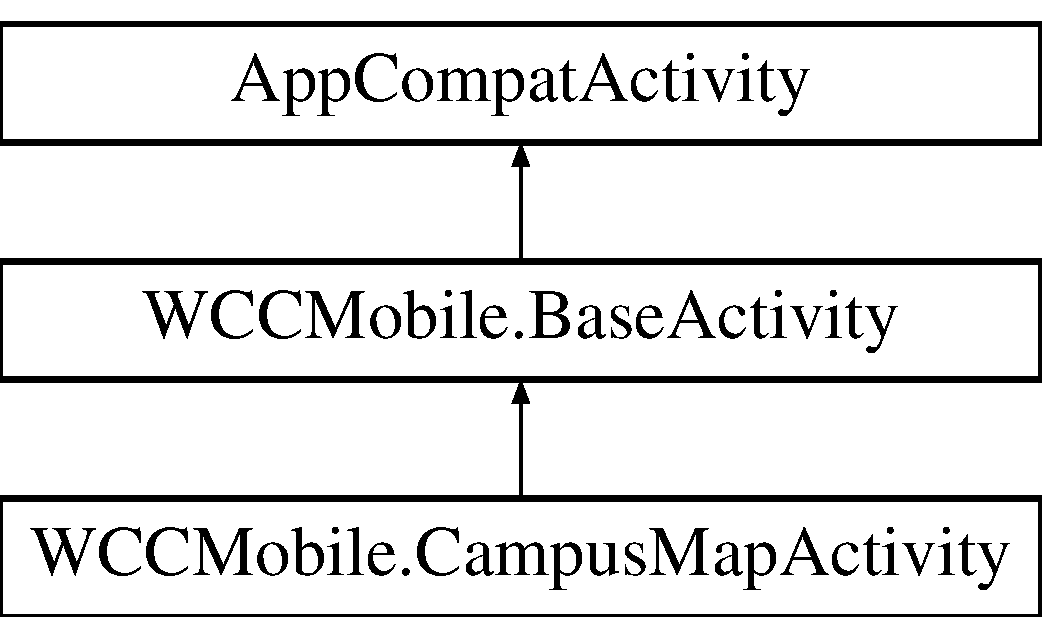
\includegraphics[height=3.000000cm]{class_w_c_c_mobile_1_1_base_activity}
\end{center}
\end{figure}
\subsection*{Protected Member Functions}
\begin{DoxyCompactItemize}
\item 
override void \hyperlink{class_w_c_c_mobile_1_1_base_activity_a19bcbf31bee5a7281a320ac674da97de}{On\+Create} (Bundle bundle)
\begin{DoxyCompactList}\small\item\em Called when \mbox{[}create\mbox{]}. \end{DoxyCompactList}\end{DoxyCompactItemize}
\subsection*{Properties}
\begin{DoxyCompactItemize}
\item 
Toolbar \hyperlink{class_w_c_c_mobile_1_1_base_activity_a2a28b22e5e08da4a6a10debd119a9c97}{Toolbar}\hspace{0.3cm}{\ttfamily  \mbox{[}get, set\mbox{]}}
\begin{DoxyCompactList}\small\item\em Gets or sets the toolbar. \end{DoxyCompactList}\item 
abstract int \hyperlink{class_w_c_c_mobile_1_1_base_activity_a982e69396d64fad1bbf643c2874c0cbd}{Layout\+Resource}\hspace{0.3cm}{\ttfamily  \mbox{[}get\mbox{]}}
\begin{DoxyCompactList}\small\item\em Gets the layout resource. \end{DoxyCompactList}\item 
int \hyperlink{class_w_c_c_mobile_1_1_base_activity_a3774a3ded238f234fdc92089a16636fa}{Action\+Bar\+Icon}\hspace{0.3cm}{\ttfamily  \mbox{[}set\mbox{]}}
\begin{DoxyCompactList}\small\item\em Sets the action bar icon. \end{DoxyCompactList}\end{DoxyCompactItemize}


\subsection{Member Function Documentation}
\index{W\+C\+C\+Mobile\+::\+Base\+Activity@{W\+C\+C\+Mobile\+::\+Base\+Activity}!On\+Create@{On\+Create}}
\index{On\+Create@{On\+Create}!W\+C\+C\+Mobile\+::\+Base\+Activity@{W\+C\+C\+Mobile\+::\+Base\+Activity}}
\subsubsection[{\texorpdfstring{On\+Create(\+Bundle bundle)}{OnCreate(Bundle bundle)}}]{\setlength{\rightskip}{0pt plus 5cm}override void W\+C\+C\+Mobile.\+Base\+Activity.\+On\+Create (
\begin{DoxyParamCaption}
\item[{Bundle}]{bundle}
\end{DoxyParamCaption}
)\hspace{0.3cm}{\ttfamily [protected]}}\hypertarget{class_w_c_c_mobile_1_1_base_activity_a19bcbf31bee5a7281a320ac674da97de}{}\label{class_w_c_c_mobile_1_1_base_activity_a19bcbf31bee5a7281a320ac674da97de}


Called when \mbox{[}create\mbox{]}. 


\begin{DoxyParams}{Parameters}
{\em bundle} & The bundle.\\
\hline
\end{DoxyParams}


\subsection{Property Documentation}
\index{W\+C\+C\+Mobile\+::\+Base\+Activity@{W\+C\+C\+Mobile\+::\+Base\+Activity}!Action\+Bar\+Icon@{Action\+Bar\+Icon}}
\index{Action\+Bar\+Icon@{Action\+Bar\+Icon}!W\+C\+C\+Mobile\+::\+Base\+Activity@{W\+C\+C\+Mobile\+::\+Base\+Activity}}
\subsubsection[{\texorpdfstring{Action\+Bar\+Icon}{ActionBarIcon}}]{\setlength{\rightskip}{0pt plus 5cm}int W\+C\+C\+Mobile.\+Base\+Activity.\+Action\+Bar\+Icon\hspace{0.3cm}{\ttfamily [set]}, {\ttfamily [protected]}}\hypertarget{class_w_c_c_mobile_1_1_base_activity_a3774a3ded238f234fdc92089a16636fa}{}\label{class_w_c_c_mobile_1_1_base_activity_a3774a3ded238f234fdc92089a16636fa}


Sets the action bar icon. 

The action bar icon. \index{W\+C\+C\+Mobile\+::\+Base\+Activity@{W\+C\+C\+Mobile\+::\+Base\+Activity}!Layout\+Resource@{Layout\+Resource}}
\index{Layout\+Resource@{Layout\+Resource}!W\+C\+C\+Mobile\+::\+Base\+Activity@{W\+C\+C\+Mobile\+::\+Base\+Activity}}
\subsubsection[{\texorpdfstring{Layout\+Resource}{LayoutResource}}]{\setlength{\rightskip}{0pt plus 5cm}abstract int W\+C\+C\+Mobile.\+Base\+Activity.\+Layout\+Resource\hspace{0.3cm}{\ttfamily [get]}, {\ttfamily [protected]}}\hypertarget{class_w_c_c_mobile_1_1_base_activity_a982e69396d64fad1bbf643c2874c0cbd}{}\label{class_w_c_c_mobile_1_1_base_activity_a982e69396d64fad1bbf643c2874c0cbd}


Gets the layout resource. 

The layout resource. \index{W\+C\+C\+Mobile\+::\+Base\+Activity@{W\+C\+C\+Mobile\+::\+Base\+Activity}!Toolbar@{Toolbar}}
\index{Toolbar@{Toolbar}!W\+C\+C\+Mobile\+::\+Base\+Activity@{W\+C\+C\+Mobile\+::\+Base\+Activity}}
\subsubsection[{\texorpdfstring{Toolbar}{Toolbar}}]{\setlength{\rightskip}{0pt plus 5cm}Toolbar W\+C\+C\+Mobile.\+Base\+Activity.\+Toolbar\hspace{0.3cm}{\ttfamily [get]}, {\ttfamily [set]}}\hypertarget{class_w_c_c_mobile_1_1_base_activity_a2a28b22e5e08da4a6a10debd119a9c97}{}\label{class_w_c_c_mobile_1_1_base_activity_a2a28b22e5e08da4a6a10debd119a9c97}


Gets or sets the toolbar. 

The toolbar. 

The documentation for this class was generated from the following file\+:\begin{DoxyCompactItemize}
\item 
Source/\+Activities/Base\+Activity.\+cs\end{DoxyCompactItemize}

\hypertarget{class_w_c_c_mobile_1_1_adapters_1_1_base_populate_view_holder}{}\section{W\+C\+C\+Mobile.\+Adapters.\+Base\+Populate\+View\+Holder$<$ T $>$ Class Template Reference}
\label{class_w_c_c_mobile_1_1_adapters_1_1_base_populate_view_holder}\index{W\+C\+C\+Mobile.\+Adapters.\+Base\+Populate\+View\+Holder$<$ T $>$@{W\+C\+C\+Mobile.\+Adapters.\+Base\+Populate\+View\+Holder$<$ T $>$}}
Inheritance diagram for W\+C\+C\+Mobile.\+Adapters.\+Base\+Populate\+View\+Holder$<$ T $>$\+:\begin{figure}[H]
\begin{center}
\leavevmode
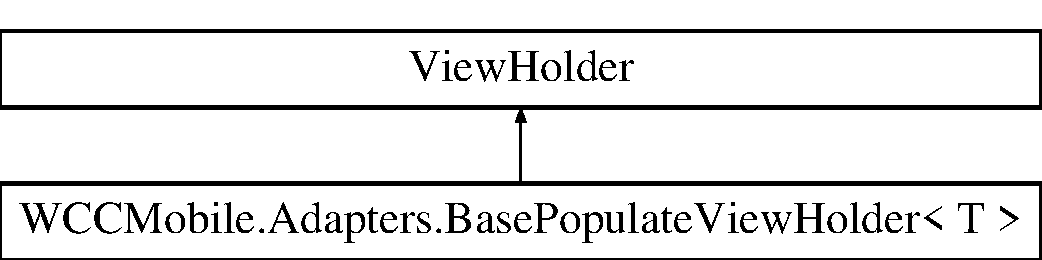
\includegraphics[height=2.000000cm]{class_w_c_c_mobile_1_1_adapters_1_1_base_populate_view_holder}
\end{center}
\end{figure}
\subsection*{Public Member Functions}
\begin{DoxyCompactItemize}
\item 
abstract void \hyperlink{class_w_c_c_mobile_1_1_adapters_1_1_base_populate_view_holder_aa4fb01d73390980ec2d122ddc4d1739c}{Populate\+From} (T data)
\begin{DoxyCompactList}\small\item\em Populates overriding children of \hyperlink{class_w_c_c_mobile_1_1_adapters_1_1_base_populate_view_holder_a633bdb266d578bee85e40840b2905593}{Base\+Populate\+View\+Holder$<$\+T$>$} with {\itshape data} . \end{DoxyCompactList}\item 
\hyperlink{class_w_c_c_mobile_1_1_adapters_1_1_base_populate_view_holder_a633bdb266d578bee85e40840b2905593}{Base\+Populate\+View\+Holder} (View item\+View)
\begin{DoxyCompactList}\small\item\em Initializes a new instance of the \hyperlink{class_w_c_c_mobile_1_1_adapters_1_1_base_populate_view_holder_a633bdb266d578bee85e40840b2905593}{Base\+Populate\+View\+Holder$<$\+T$>$} class. \end{DoxyCompactList}\item 
void \hyperlink{class_w_c_c_mobile_1_1_adapters_1_1_base_populate_view_holder_a31e7627fe3cc68311934b017305f4eb9}{Set\+Click\+Listener} (Action$<$ int $>$ listener)
\begin{DoxyCompactList}\small\item\em Sets the click listener. \end{DoxyCompactList}\end{DoxyCompactItemize}
\subsection*{Protected Member Functions}
\begin{DoxyCompactItemize}
\item 
override void \hyperlink{class_w_c_c_mobile_1_1_adapters_1_1_base_populate_view_holder_a7d1e5fd331f1e61130279bab2353d164}{Dispose} (bool disposing)
\begin{DoxyCompactList}\small\item\em Releases unmanaged and -\/ optionally -\/ managed resources. \end{DoxyCompactList}\end{DoxyCompactItemize}


\subsection{Constructor \& Destructor Documentation}
\index{W\+C\+C\+Mobile\+::\+Adapters\+::\+Base\+Populate\+View\+Holder@{W\+C\+C\+Mobile\+::\+Adapters\+::\+Base\+Populate\+View\+Holder}!Base\+Populate\+View\+Holder@{Base\+Populate\+View\+Holder}}
\index{Base\+Populate\+View\+Holder@{Base\+Populate\+View\+Holder}!W\+C\+C\+Mobile\+::\+Adapters\+::\+Base\+Populate\+View\+Holder@{W\+C\+C\+Mobile\+::\+Adapters\+::\+Base\+Populate\+View\+Holder}}
\subsubsection[{\texorpdfstring{Base\+Populate\+View\+Holder(\+View item\+View)}{BasePopulateViewHolder(View itemView)}}]{\setlength{\rightskip}{0pt plus 5cm}{\bf W\+C\+C\+Mobile.\+Adapters.\+Base\+Populate\+View\+Holder}$<$ T $>$.{\bf Base\+Populate\+View\+Holder} (
\begin{DoxyParamCaption}
\item[{View}]{item\+View}
\end{DoxyParamCaption}
)}\hypertarget{class_w_c_c_mobile_1_1_adapters_1_1_base_populate_view_holder_a633bdb266d578bee85e40840b2905593}{}\label{class_w_c_c_mobile_1_1_adapters_1_1_base_populate_view_holder_a633bdb266d578bee85e40840b2905593}


Initializes a new instance of the \hyperlink{class_w_c_c_mobile_1_1_adapters_1_1_base_populate_view_holder_a633bdb266d578bee85e40840b2905593}{Base\+Populate\+View\+Holder$<$\+T$>$} class. 


\begin{DoxyParams}{Parameters}
{\em item\+View} & The item view.\\
\hline
\end{DoxyParams}


\subsection{Member Function Documentation}
\index{W\+C\+C\+Mobile\+::\+Adapters\+::\+Base\+Populate\+View\+Holder@{W\+C\+C\+Mobile\+::\+Adapters\+::\+Base\+Populate\+View\+Holder}!Dispose@{Dispose}}
\index{Dispose@{Dispose}!W\+C\+C\+Mobile\+::\+Adapters\+::\+Base\+Populate\+View\+Holder@{W\+C\+C\+Mobile\+::\+Adapters\+::\+Base\+Populate\+View\+Holder}}
\subsubsection[{\texorpdfstring{Dispose(bool disposing)}{Dispose(bool disposing)}}]{\setlength{\rightskip}{0pt plus 5cm}override void {\bf W\+C\+C\+Mobile.\+Adapters.\+Base\+Populate\+View\+Holder}$<$ T $>$.Dispose (
\begin{DoxyParamCaption}
\item[{bool}]{disposing}
\end{DoxyParamCaption}
)\hspace{0.3cm}{\ttfamily [protected]}}\hypertarget{class_w_c_c_mobile_1_1_adapters_1_1_base_populate_view_holder_a7d1e5fd331f1e61130279bab2353d164}{}\label{class_w_c_c_mobile_1_1_adapters_1_1_base_populate_view_holder_a7d1e5fd331f1e61130279bab2353d164}


Releases unmanaged and -\/ optionally -\/ managed resources. 


\begin{DoxyParams}{Parameters}
{\em disposing} & {\ttfamily true} to release both managed and unmanaged resources; {\ttfamily false} to release only unmanaged resources.\\
\hline
\end{DoxyParams}
\index{W\+C\+C\+Mobile\+::\+Adapters\+::\+Base\+Populate\+View\+Holder@{W\+C\+C\+Mobile\+::\+Adapters\+::\+Base\+Populate\+View\+Holder}!Populate\+From@{Populate\+From}}
\index{Populate\+From@{Populate\+From}!W\+C\+C\+Mobile\+::\+Adapters\+::\+Base\+Populate\+View\+Holder@{W\+C\+C\+Mobile\+::\+Adapters\+::\+Base\+Populate\+View\+Holder}}
\subsubsection[{\texorpdfstring{Populate\+From(\+T data)}{PopulateFrom(T data)}}]{\setlength{\rightskip}{0pt plus 5cm}abstract void {\bf W\+C\+C\+Mobile.\+Adapters.\+Base\+Populate\+View\+Holder}$<$ T $>$.Populate\+From (
\begin{DoxyParamCaption}
\item[{T}]{data}
\end{DoxyParamCaption}
)\hspace{0.3cm}{\ttfamily [pure virtual]}}\hypertarget{class_w_c_c_mobile_1_1_adapters_1_1_base_populate_view_holder_aa4fb01d73390980ec2d122ddc4d1739c}{}\label{class_w_c_c_mobile_1_1_adapters_1_1_base_populate_view_holder_aa4fb01d73390980ec2d122ddc4d1739c}


Populates overriding children of \hyperlink{class_w_c_c_mobile_1_1_adapters_1_1_base_populate_view_holder_a633bdb266d578bee85e40840b2905593}{Base\+Populate\+View\+Holder$<$\+T$>$} with {\itshape data} . 


\begin{DoxyParams}{Parameters}
{\em data} & The data.\\
\hline
\end{DoxyParams}
\index{W\+C\+C\+Mobile\+::\+Adapters\+::\+Base\+Populate\+View\+Holder@{W\+C\+C\+Mobile\+::\+Adapters\+::\+Base\+Populate\+View\+Holder}!Set\+Click\+Listener@{Set\+Click\+Listener}}
\index{Set\+Click\+Listener@{Set\+Click\+Listener}!W\+C\+C\+Mobile\+::\+Adapters\+::\+Base\+Populate\+View\+Holder@{W\+C\+C\+Mobile\+::\+Adapters\+::\+Base\+Populate\+View\+Holder}}
\subsubsection[{\texorpdfstring{Set\+Click\+Listener(\+Action$<$ int $>$ listener)}{SetClickListener(Action< int > listener)}}]{\setlength{\rightskip}{0pt plus 5cm}void {\bf W\+C\+C\+Mobile.\+Adapters.\+Base\+Populate\+View\+Holder}$<$ T $>$.Set\+Click\+Listener (
\begin{DoxyParamCaption}
\item[{Action$<$ int $>$}]{listener}
\end{DoxyParamCaption}
)}\hypertarget{class_w_c_c_mobile_1_1_adapters_1_1_base_populate_view_holder_a31e7627fe3cc68311934b017305f4eb9}{}\label{class_w_c_c_mobile_1_1_adapters_1_1_base_populate_view_holder_a31e7627fe3cc68311934b017305f4eb9}


Sets the click listener. 


\begin{DoxyParams}{Parameters}
{\em listener} & The listener.\\
\hline
\end{DoxyParams}


The documentation for this class was generated from the following file\+:\begin{DoxyCompactItemize}
\item 
Source/\+Adapters/Generic\+Adapter.\+cs\end{DoxyCompactItemize}

\hypertarget{class_w_c_c_mobile_1_1_basic_info_activity}{}\section{W\+C\+C\+Mobile.\+Basic\+Info\+Activity Class Reference}
\label{class_w_c_c_mobile_1_1_basic_info_activity}\index{W\+C\+C\+Mobile.\+Basic\+Info\+Activity@{W\+C\+C\+Mobile.\+Basic\+Info\+Activity}}
Inheritance diagram for W\+C\+C\+Mobile.\+Basic\+Info\+Activity\+:\begin{figure}[H]
\begin{center}
\leavevmode
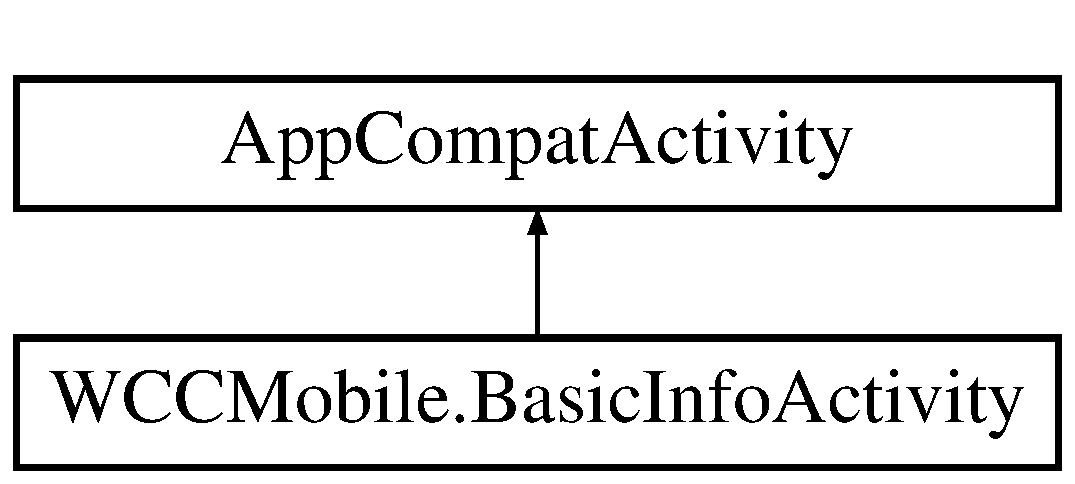
\includegraphics[height=2.000000cm]{class_w_c_c_mobile_1_1_basic_info_activity}
\end{center}
\end{figure}
\subsection*{Public Member Functions}
\begin{DoxyCompactItemize}
\item 
override bool {\bfseries On\+Options\+Item\+Selected} (I\+Menu\+Item item)\hypertarget{class_w_c_c_mobile_1_1_basic_info_activity_a5fd28198ec622865064002f9f343e1e5}{}\label{class_w_c_c_mobile_1_1_basic_info_activity_a5fd28198ec622865064002f9f343e1e5}

\end{DoxyCompactItemize}
\subsection*{Static Public Member Functions}
\begin{DoxyCompactItemize}
\item 
static void {\bfseries set\+Info\+Title} (string new\+Title)\hypertarget{class_w_c_c_mobile_1_1_basic_info_activity_aef49547da4fca04a6556220c3b5c2808}{}\label{class_w_c_c_mobile_1_1_basic_info_activity_aef49547da4fca04a6556220c3b5c2808}

\end{DoxyCompactItemize}
\subsection*{Protected Member Functions}
\begin{DoxyCompactItemize}
\item 
override void {\bfseries On\+Create} (Bundle saved\+Instance\+State)\hypertarget{class_w_c_c_mobile_1_1_basic_info_activity_aedceea6ca307d1d3d37d0c06460621e8}{}\label{class_w_c_c_mobile_1_1_basic_info_activity_aedceea6ca307d1d3d37d0c06460621e8}

\end{DoxyCompactItemize}


The documentation for this class was generated from the following file\+:\begin{DoxyCompactItemize}
\item 
Source/\+Activities/Basic\+Info\+Activity.\+cs\end{DoxyCompactItemize}

\hypertarget{class_w_c_c_mobile_1_1_bitmap_cache}{}\section{W\+C\+C\+Mobile.\+Bitmap\+Cache Class Reference}
\label{class_w_c_c_mobile_1_1_bitmap_cache}\index{W\+C\+C\+Mobile.\+Bitmap\+Cache@{W\+C\+C\+Mobile.\+Bitmap\+Cache}}
\subsection*{Public Member Functions}
\begin{DoxyCompactItemize}
\item 
void \hyperlink{class_w_c_c_mobile_1_1_bitmap_cache_abc1bb6bb92fae6341a28be220ef526b5}{Add\+Or\+Update} (string key, Bitmap bitmap, Time\+Span duration)
\begin{DoxyCompactList}\small\item\em Adds or updates the {\itshape bitmap} . \end{DoxyCompactList}\item 
bool \hyperlink{class_w_c_c_mobile_1_1_bitmap_cache_aef6dc59115bd31284061164824016b48}{Try\+Get} (string key, out Bitmap bitmap)
\begin{DoxyCompactList}\small\item\em Get\textquotesingle{}s the {\itshape bitmap}  associated with the {\itshape key} . \end{DoxyCompactList}\end{DoxyCompactItemize}
\subsection*{Static Public Member Functions}
\begin{DoxyCompactItemize}
\item 
static \hyperlink{class_w_c_c_mobile_1_1_bitmap_cache}{Bitmap\+Cache} \hyperlink{class_w_c_c_mobile_1_1_bitmap_cache_a82500ffb74a2f16fac9f59b385cd7ee6}{Create\+Cache} (Android.\+Content.\+Context context, string cache\+Name, string version=\char`\"{}1.\+0\char`\"{})
\begin{DoxyCompactList}\small\item\em Creates the cache. \end{DoxyCompactList}\end{DoxyCompactItemize}


\subsection{Member Function Documentation}
\index{W\+C\+C\+Mobile\+::\+Bitmap\+Cache@{W\+C\+C\+Mobile\+::\+Bitmap\+Cache}!Add\+Or\+Update@{Add\+Or\+Update}}
\index{Add\+Or\+Update@{Add\+Or\+Update}!W\+C\+C\+Mobile\+::\+Bitmap\+Cache@{W\+C\+C\+Mobile\+::\+Bitmap\+Cache}}
\subsubsection[{\texorpdfstring{Add\+Or\+Update(string key, Bitmap bitmap, Time\+Span duration)}{AddOrUpdate(string key, Bitmap bitmap, TimeSpan duration)}}]{\setlength{\rightskip}{0pt plus 5cm}void W\+C\+C\+Mobile.\+Bitmap\+Cache.\+Add\+Or\+Update (
\begin{DoxyParamCaption}
\item[{string}]{key, }
\item[{Bitmap}]{bitmap, }
\item[{Time\+Span}]{duration}
\end{DoxyParamCaption}
)}\hypertarget{class_w_c_c_mobile_1_1_bitmap_cache_abc1bb6bb92fae6341a28be220ef526b5}{}\label{class_w_c_c_mobile_1_1_bitmap_cache_abc1bb6bb92fae6341a28be220ef526b5}


Adds or updates the {\itshape bitmap} . 


\begin{DoxyParams}{Parameters}
{\em key} & The key.\\
\hline
{\em bmp} & The B\+MP.\\
\hline
{\em duration} & The duration.\\
\hline
\end{DoxyParams}
\index{W\+C\+C\+Mobile\+::\+Bitmap\+Cache@{W\+C\+C\+Mobile\+::\+Bitmap\+Cache}!Create\+Cache@{Create\+Cache}}
\index{Create\+Cache@{Create\+Cache}!W\+C\+C\+Mobile\+::\+Bitmap\+Cache@{W\+C\+C\+Mobile\+::\+Bitmap\+Cache}}
\subsubsection[{\texorpdfstring{Create\+Cache(\+Android.\+Content.\+Context context, string cache\+Name, string version=""1.\+0"")}{CreateCache(Android.Content.Context context, string cacheName, string version="1.0")}}]{\setlength{\rightskip}{0pt plus 5cm}static {\bf Bitmap\+Cache} W\+C\+C\+Mobile.\+Bitmap\+Cache.\+Create\+Cache (
\begin{DoxyParamCaption}
\item[{Android.\+Content.\+Context}]{context, }
\item[{string}]{cache\+Name, }
\item[{string}]{version = {\ttfamily \char`\"{}1.0\char`\"{}}}
\end{DoxyParamCaption}
)\hspace{0.3cm}{\ttfamily [static]}}\hypertarget{class_w_c_c_mobile_1_1_bitmap_cache_a82500ffb74a2f16fac9f59b385cd7ee6}{}\label{class_w_c_c_mobile_1_1_bitmap_cache_a82500ffb74a2f16fac9f59b385cd7ee6}


Creates the cache. 


\begin{DoxyParams}{Parameters}
{\em ctx} & The context.\\
\hline
{\em cache\+Name} & Name of the cache.\\
\hline
{\em version} & The version.\\
\hline
\end{DoxyParams}
\begin{DoxyReturn}{Returns}

\end{DoxyReturn}
\index{W\+C\+C\+Mobile\+::\+Bitmap\+Cache@{W\+C\+C\+Mobile\+::\+Bitmap\+Cache}!Try\+Get@{Try\+Get}}
\index{Try\+Get@{Try\+Get}!W\+C\+C\+Mobile\+::\+Bitmap\+Cache@{W\+C\+C\+Mobile\+::\+Bitmap\+Cache}}
\subsubsection[{\texorpdfstring{Try\+Get(string key, out Bitmap bitmap)}{TryGet(string key, out Bitmap bitmap)}}]{\setlength{\rightskip}{0pt plus 5cm}bool W\+C\+C\+Mobile.\+Bitmap\+Cache.\+Try\+Get (
\begin{DoxyParamCaption}
\item[{string}]{key, }
\item[{out Bitmap}]{bitmap}
\end{DoxyParamCaption}
)}\hypertarget{class_w_c_c_mobile_1_1_bitmap_cache_aef6dc59115bd31284061164824016b48}{}\label{class_w_c_c_mobile_1_1_bitmap_cache_aef6dc59115bd31284061164824016b48}


Get\textquotesingle{}s the {\itshape bitmap}  associated with the {\itshape key} . 


\begin{DoxyParams}{Parameters}
{\em key} & The key.\\
\hline
{\em bmp} & The B\+MP.\\
\hline
\end{DoxyParams}
\begin{DoxyReturn}{Returns}

\end{DoxyReturn}


The documentation for this class was generated from the following file\+:\begin{DoxyCompactItemize}
\item 
Source/\+Storage/Bitmap\+Cache.\+cs\end{DoxyCompactItemize}

\hypertarget{class_w_c_c_mobile_1_1_campus_map_activity}{}\section{W\+C\+C\+Mobile.\+Campus\+Map\+Activity Class Reference}
\label{class_w_c_c_mobile_1_1_campus_map_activity}\index{W\+C\+C\+Mobile.\+Campus\+Map\+Activity@{W\+C\+C\+Mobile.\+Campus\+Map\+Activity}}
Inheritance diagram for W\+C\+C\+Mobile.\+Campus\+Map\+Activity\+:\begin{figure}[H]
\begin{center}
\leavevmode
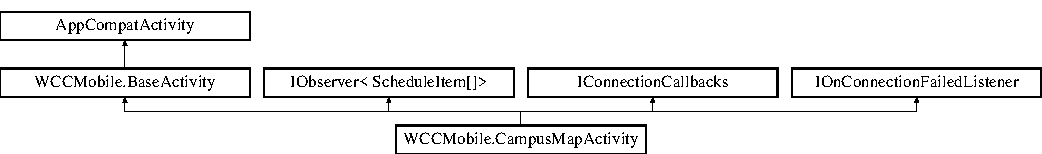
\includegraphics[height=2.068965cm]{class_w_c_c_mobile_1_1_campus_map_activity}
\end{center}
\end{figure}
\subsection*{Public Member Functions}
\begin{DoxyCompactItemize}
\item 
override void \hyperlink{class_w_c_c_mobile_1_1_campus_map_activity_a916ad58c240808114b3b7caccf5eb3ef}{On\+Configuration\+Changed} (Android.\+Content.\+Res.\+Configuration new\+Config)
\item 
override bool \hyperlink{class_w_c_c_mobile_1_1_campus_map_activity_a5691fdf085a4f060de472da2e3eba7ed}{On\+Options\+Item\+Selected} (I\+Menu\+Item item)
\begin{DoxyCompactList}\small\item\em This hook is called whenever an item in your options menu is selected. \end{DoxyCompactList}\item 
void {\bfseries On\+Completed} ()\hypertarget{class_w_c_c_mobile_1_1_campus_map_activity_a7dd1c57327ee20a030821feca778d854}{}\label{class_w_c_c_mobile_1_1_campus_map_activity_a7dd1c57327ee20a030821feca778d854}

\item 
void {\bfseries On\+Error} (Exception error)\hypertarget{class_w_c_c_mobile_1_1_campus_map_activity_a56f551e2949aeaa87c8062ae68582291}{}\label{class_w_c_c_mobile_1_1_campus_map_activity_a56f551e2949aeaa87c8062ae68582291}

\item 
void {\bfseries On\+Next} (\hyperlink{class_w_c_c_mobile_1_1_models_1_1_schedule_item}{Schedule\+Item}\mbox{[}$\,$\mbox{]} value)\hypertarget{class_w_c_c_mobile_1_1_campus_map_activity_a95ba3fa2bd54717d8ba117212ea029b7}{}\label{class_w_c_c_mobile_1_1_campus_map_activity_a95ba3fa2bd54717d8ba117212ea029b7}

\item 
void {\bfseries On\+Connected} (Bundle p0)\hypertarget{class_w_c_c_mobile_1_1_campus_map_activity_a28dd11f186a7e08687fa050b813d0769}{}\label{class_w_c_c_mobile_1_1_campus_map_activity_a28dd11f186a7e08687fa050b813d0769}

\item 
void \hyperlink{class_w_c_c_mobile_1_1_campus_map_activity_a406a3e9490fd2a158b1b2c65f7c99448}{On\+Disconnected} ()
\begin{DoxyCompactList}\small\item\em Called when \mbox{[}disconnected\mbox{]}. \end{DoxyCompactList}\item 
void \hyperlink{class_w_c_c_mobile_1_1_campus_map_activity_ab8134e37f2c53584ae6d5425876e04e8}{On\+Connection\+Failed} (Connection\+Result p0)
\begin{DoxyCompactList}\small\item\em Called when \mbox{[}connection failed\mbox{]}. \end{DoxyCompactList}\item 
void \hyperlink{class_w_c_c_mobile_1_1_campus_map_activity_a37c8fdd89fae802e8b02b3e1e3fd25d0}{On\+Connection\+Suspended} (int reason)
\begin{DoxyCompactList}\small\item\em Called when \mbox{[}connection suspended\mbox{]}. \end{DoxyCompactList}\end{DoxyCompactItemize}
\subsection*{Protected Member Functions}
\begin{DoxyCompactItemize}
\item 
override void \hyperlink{class_w_c_c_mobile_1_1_campus_map_activity_aeb984dffcd2273acbfa613b77463ab41}{On\+Create} (Bundle bundle)
\begin{DoxyCompactList}\small\item\em Called when \mbox{[}create\mbox{]}. \end{DoxyCompactList}\item 
override void \hyperlink{class_w_c_c_mobile_1_1_campus_map_activity_a1af9a9440cd61b261be8493a7fad7d3c}{On\+Post\+Create} (Bundle saved\+Instance\+State)
\item 
override void \hyperlink{class_w_c_c_mobile_1_1_campus_map_activity_a2c2b911fee48f83a49b5924ab94b74db}{On\+New\+Intent} (Intent intent)
\begin{DoxyCompactList}\small\item\em This is called for activities that set launch\+Mode to \char`\"{}single\+Top\char`\"{} in their package, or if a client used the {\ttfamily F\+:\+Android.\+Content.\+Activity\+Flags.\+Single\+Top} flag when calling {\ttfamily M\+:\+Android.\+Content.\+Context\+Wrapper.\+Start\+Activity(\+Android.\+Content.\+Intent)}. \end{DoxyCompactList}\item 
override void \hyperlink{class_w_c_c_mobile_1_1_campus_map_activity_a4bdab2012ca79f06da02249206fe0a72}{On\+Start} ()
\begin{DoxyCompactList}\small\item\em Called after {\ttfamily M\+:\+Android.\+App.\+Activity.\+On\+Create(\+Android.\+O\+S.\+Bundle)} \&mdash; or after {\ttfamily M\+:\+Android.\+App.\+Activity.\+On\+Restart} when the activity had been stopped, but is now again being displayed to the user. \end{DoxyCompactList}\item 
override void \hyperlink{class_w_c_c_mobile_1_1_campus_map_activity_a2e6f92363f8a8ca49caa2962f96c2538}{On\+Stop} ()
\begin{DoxyCompactList}\small\item\em Called when you are no longer visible to the user. \end{DoxyCompactList}\item 
override void \hyperlink{class_w_c_c_mobile_1_1_campus_map_activity_a91db75c589386bb46f2e356c8c8b6623}{On\+Activity\+Result} (int request\+Code, Result result\+Code, Intent data)
\begin{DoxyCompactList}\small\item\em Called when an activity you launched exits, giving you the request\+Code you started it with, the result\+Code it returned, and any additional data from it. \end{DoxyCompactList}\end{DoxyCompactItemize}
\subsection*{Properties}
\begin{DoxyCompactItemize}
\item 
override int \hyperlink{class_w_c_c_mobile_1_1_campus_map_activity_ac93753471d106f992c78e927d3f87d1f}{Layout\+Resource}\hspace{0.3cm}{\ttfamily  \mbox{[}get\mbox{]}}
\begin{DoxyCompactList}\small\item\em Gets the layout resource. \end{DoxyCompactList}\end{DoxyCompactItemize}


\subsection{Member Function Documentation}
\index{W\+C\+C\+Mobile\+::\+Campus\+Map\+Activity@{W\+C\+C\+Mobile\+::\+Campus\+Map\+Activity}!On\+Activity\+Result@{On\+Activity\+Result}}
\index{On\+Activity\+Result@{On\+Activity\+Result}!W\+C\+C\+Mobile\+::\+Campus\+Map\+Activity@{W\+C\+C\+Mobile\+::\+Campus\+Map\+Activity}}
\subsubsection[{\texorpdfstring{On\+Activity\+Result(int request\+Code, Result result\+Code, Intent data)}{OnActivityResult(int requestCode, Result resultCode, Intent data)}}]{\setlength{\rightskip}{0pt plus 5cm}override void W\+C\+C\+Mobile.\+Campus\+Map\+Activity.\+On\+Activity\+Result (
\begin{DoxyParamCaption}
\item[{int}]{request\+Code, }
\item[{Result}]{result\+Code, }
\item[{Intent}]{data}
\end{DoxyParamCaption}
)\hspace{0.3cm}{\ttfamily [protected]}}\hypertarget{class_w_c_c_mobile_1_1_campus_map_activity_a91db75c589386bb46f2e356c8c8b6623}{}\label{class_w_c_c_mobile_1_1_campus_map_activity_a91db75c589386bb46f2e356c8c8b6623}


Called when an activity you launched exits, giving you the request\+Code you started it with, the result\+Code it returned, and any additional data from it. 


\begin{DoxyParams}{Parameters}
{\em request\+Code} & The integer request code originally supplied to start\+Activity\+For\+Result(), allowing you to identify who this result came from.\\
\hline
{\em result\+Code} & The integer result code returned by the child activity through its set\+Result().\\
\hline
{\em data} & An Intent, which can return result data to the caller (various data can be attached to Intent \char`\"{}extras\char`\"{}).\\
\hline
\end{DoxyParams}


Called when an activity you launched exits, giving you the request\+Code you started it with, the result\+Code it returned, and any additional data from it. The $<$format type=\char`\"{}text/html\char`\"{}$>${\itshape result\+Code}$<$/format$>$ will be {\ttfamily F\+:\+Android.\+App.\+Result.\+Canceled} if the activity explicitly returned that, didn\textquotesingle{}t return any result, or crashed during its operation. 

You will receive this call immediately before on\+Resume() when your activity is re-\/starting.

$<$format type=\char`\"{}text/html\char`\"{}$>$ \href{http://developer.android.com/reference/android/app/Activity.html#onActivityResult(int, int, android.content.Intent)}{\tt \mbox{[}Android Documentation\mbox{]}} $<$/format$>$ 

$<$since version=\char`\"{}\+Added in A\+P\+I level 1\char`\"{}$>$ $<$altmember cref=\char`\"{}\+M\+:\+Android.\+App.\+Activity.\+Start\+Activity\+For\+Result(\+Android.\+Content.\+Intent, System.\+Int32)\char`\"{}$>$ $<$altmember cref=\char`\"{}\+M\+:\+Android.\+App.\+Activity.\+Create\+Pending\+Result(\+System.\+Int32, Android.\+Content.\+Intent, Android.\+Content.\+Intent)\char`\"{}$>$ $<$altmember cref=\char`\"{}\+M\+:\+Android.\+App.\+Activity.\+Set\+Result(\+Android.\+App.\+Result)\char`\"{}$>$ \index{W\+C\+C\+Mobile\+::\+Campus\+Map\+Activity@{W\+C\+C\+Mobile\+::\+Campus\+Map\+Activity}!On\+Configuration\+Changed@{On\+Configuration\+Changed}}
\index{On\+Configuration\+Changed@{On\+Configuration\+Changed}!W\+C\+C\+Mobile\+::\+Campus\+Map\+Activity@{W\+C\+C\+Mobile\+::\+Campus\+Map\+Activity}}
\subsubsection[{\texorpdfstring{On\+Configuration\+Changed(\+Android.\+Content.\+Res.\+Configuration new\+Config)}{OnConfigurationChanged(Android.Content.Res.Configuration newConfig)}}]{\setlength{\rightskip}{0pt plus 5cm}override void W\+C\+C\+Mobile.\+Campus\+Map\+Activity.\+On\+Configuration\+Changed (
\begin{DoxyParamCaption}
\item[{Android.\+Content.\+Res.\+Configuration}]{new\+Config}
\end{DoxyParamCaption}
)}\hypertarget{class_w_c_c_mobile_1_1_campus_map_activity_a916ad58c240808114b3b7caccf5eb3ef}{}\label{class_w_c_c_mobile_1_1_campus_map_activity_a916ad58c240808114b3b7caccf5eb3ef}




Called by the system when the device configuration changes while your activity is running. 


\begin{DoxyParams}{Parameters}
{\em new\+Config} & The new device configuration.\\
\hline
\end{DoxyParams}


Called by the system when the device configuration changes while your activity is running. Note that this will {\itshape only} be called if you have selected configurations you would like to handle with the {\ttfamily F\+:\+Android.\+Resource.\+Attribute.\+Config\+Changes} attribute in your manifest. If any configuration change occurs that is not selected to be reported by that attribute, then instead of reporting it the system will stop and restart the activity (to have it launched with the new configuration). 

At the time that this function has been called, your \hyperlink{namespace_w_c_c_mobile_1_1_resources}{Resources} object will have been updated to return resource values matching the new configuration.

$<$format type=\char`\"{}text/html\char`\"{}$>$ \href{http://developer.android.com/reference/android/app/Activity.html#onConfigurationChanged(android.content.res.Configuration)}{\tt \mbox{[}Android Documentation\mbox{]}} $<$/format$>$ 

$<$since version=\char`\"{}\+Added in A\+P\+I level 1\char`\"{}$>$ \index{W\+C\+C\+Mobile\+::\+Campus\+Map\+Activity@{W\+C\+C\+Mobile\+::\+Campus\+Map\+Activity}!On\+Connection\+Failed@{On\+Connection\+Failed}}
\index{On\+Connection\+Failed@{On\+Connection\+Failed}!W\+C\+C\+Mobile\+::\+Campus\+Map\+Activity@{W\+C\+C\+Mobile\+::\+Campus\+Map\+Activity}}
\subsubsection[{\texorpdfstring{On\+Connection\+Failed(\+Connection\+Result p0)}{OnConnectionFailed(ConnectionResult p0)}}]{\setlength{\rightskip}{0pt plus 5cm}void W\+C\+C\+Mobile.\+Campus\+Map\+Activity.\+On\+Connection\+Failed (
\begin{DoxyParamCaption}
\item[{Connection\+Result}]{p0}
\end{DoxyParamCaption}
)}\hypertarget{class_w_c_c_mobile_1_1_campus_map_activity_ab8134e37f2c53584ae6d5425876e04e8}{}\label{class_w_c_c_mobile_1_1_campus_map_activity_ab8134e37f2c53584ae6d5425876e04e8}


Called when \mbox{[}connection failed\mbox{]}. 


\begin{DoxyParams}{Parameters}
{\em p0} & The p0.\\
\hline
\end{DoxyParams}
\index{W\+C\+C\+Mobile\+::\+Campus\+Map\+Activity@{W\+C\+C\+Mobile\+::\+Campus\+Map\+Activity}!On\+Connection\+Suspended@{On\+Connection\+Suspended}}
\index{On\+Connection\+Suspended@{On\+Connection\+Suspended}!W\+C\+C\+Mobile\+::\+Campus\+Map\+Activity@{W\+C\+C\+Mobile\+::\+Campus\+Map\+Activity}}
\subsubsection[{\texorpdfstring{On\+Connection\+Suspended(int reason)}{OnConnectionSuspended(int reason)}}]{\setlength{\rightskip}{0pt plus 5cm}void W\+C\+C\+Mobile.\+Campus\+Map\+Activity.\+On\+Connection\+Suspended (
\begin{DoxyParamCaption}
\item[{int}]{reason}
\end{DoxyParamCaption}
)}\hypertarget{class_w_c_c_mobile_1_1_campus_map_activity_a37c8fdd89fae802e8b02b3e1e3fd25d0}{}\label{class_w_c_c_mobile_1_1_campus_map_activity_a37c8fdd89fae802e8b02b3e1e3fd25d0}


Called when \mbox{[}connection suspended\mbox{]}. 


\begin{DoxyParams}{Parameters}
{\em reason} & The reason.\\
\hline
\end{DoxyParams}
\index{W\+C\+C\+Mobile\+::\+Campus\+Map\+Activity@{W\+C\+C\+Mobile\+::\+Campus\+Map\+Activity}!On\+Create@{On\+Create}}
\index{On\+Create@{On\+Create}!W\+C\+C\+Mobile\+::\+Campus\+Map\+Activity@{W\+C\+C\+Mobile\+::\+Campus\+Map\+Activity}}
\subsubsection[{\texorpdfstring{On\+Create(\+Bundle bundle)}{OnCreate(Bundle bundle)}}]{\setlength{\rightskip}{0pt plus 5cm}override void W\+C\+C\+Mobile.\+Campus\+Map\+Activity.\+On\+Create (
\begin{DoxyParamCaption}
\item[{Bundle}]{bundle}
\end{DoxyParamCaption}
)\hspace{0.3cm}{\ttfamily [protected]}}\hypertarget{class_w_c_c_mobile_1_1_campus_map_activity_aeb984dffcd2273acbfa613b77463ab41}{}\label{class_w_c_c_mobile_1_1_campus_map_activity_aeb984dffcd2273acbfa613b77463ab41}


Called when \mbox{[}create\mbox{]}. 


\begin{DoxyParams}{Parameters}
{\em bundle} & The bundle.\\
\hline
\end{DoxyParams}
\index{W\+C\+C\+Mobile\+::\+Campus\+Map\+Activity@{W\+C\+C\+Mobile\+::\+Campus\+Map\+Activity}!On\+Disconnected@{On\+Disconnected}}
\index{On\+Disconnected@{On\+Disconnected}!W\+C\+C\+Mobile\+::\+Campus\+Map\+Activity@{W\+C\+C\+Mobile\+::\+Campus\+Map\+Activity}}
\subsubsection[{\texorpdfstring{On\+Disconnected()}{OnDisconnected()}}]{\setlength{\rightskip}{0pt plus 5cm}void W\+C\+C\+Mobile.\+Campus\+Map\+Activity.\+On\+Disconnected (
\begin{DoxyParamCaption}
{}
\end{DoxyParamCaption}
)}\hypertarget{class_w_c_c_mobile_1_1_campus_map_activity_a406a3e9490fd2a158b1b2c65f7c99448}{}\label{class_w_c_c_mobile_1_1_campus_map_activity_a406a3e9490fd2a158b1b2c65f7c99448}


Called when \mbox{[}disconnected\mbox{]}. 

\index{W\+C\+C\+Mobile\+::\+Campus\+Map\+Activity@{W\+C\+C\+Mobile\+::\+Campus\+Map\+Activity}!On\+New\+Intent@{On\+New\+Intent}}
\index{On\+New\+Intent@{On\+New\+Intent}!W\+C\+C\+Mobile\+::\+Campus\+Map\+Activity@{W\+C\+C\+Mobile\+::\+Campus\+Map\+Activity}}
\subsubsection[{\texorpdfstring{On\+New\+Intent(\+Intent intent)}{OnNewIntent(Intent intent)}}]{\setlength{\rightskip}{0pt plus 5cm}override void W\+C\+C\+Mobile.\+Campus\+Map\+Activity.\+On\+New\+Intent (
\begin{DoxyParamCaption}
\item[{Intent}]{intent}
\end{DoxyParamCaption}
)\hspace{0.3cm}{\ttfamily [protected]}}\hypertarget{class_w_c_c_mobile_1_1_campus_map_activity_a2c2b911fee48f83a49b5924ab94b74db}{}\label{class_w_c_c_mobile_1_1_campus_map_activity_a2c2b911fee48f83a49b5924ab94b74db}


This is called for activities that set launch\+Mode to \char`\"{}single\+Top\char`\"{} in their package, or if a client used the {\ttfamily F\+:\+Android.\+Content.\+Activity\+Flags.\+Single\+Top} flag when calling {\ttfamily M\+:\+Android.\+Content.\+Context\+Wrapper.\+Start\+Activity(\+Android.\+Content.\+Intent)}. 


\begin{DoxyParams}{Parameters}
{\em intent} & The new intent that was started for the activity.\\
\hline
\end{DoxyParams}


This is called for activities that set launch\+Mode to \char`\"{}single\+Top\char`\"{} in their package, or if a client used the {\ttfamily F\+:\+Android.\+Content.\+Activity\+Flags.\+Single\+Top} flag when calling {\ttfamily M\+:\+Android.\+Content.\+Context\+Wrapper.\+Start\+Activity(\+Android.\+Content.\+Intent)}. In either case, when the activity is re-\/launched while at the top of the activity stack instead of a new instance of the activity being started, on\+New\+Intent() will be called on the existing instance with the Intent that was used to re-\/launch it. 

An activity will always be paused before receiving a new intent, so you can count on {\ttfamily M\+:\+Android.\+App.\+Activity.\+On\+Resume} being called after this method. 

Note that {\ttfamily P\+:\+Android.\+App.\+Activity.\+Intent} still returns the original Intent. You can use {\ttfamily P\+:\+Android.\+App.\+Activity.\+Intent} to update it to this new Intent.

$<$format type=\char`\"{}text/html\char`\"{}$>$ \href{http://developer.android.com/reference/android/app/Activity.html#onNewIntent(android.content.Intent)}{\tt \mbox{[}Android Documentation\mbox{]}} $<$/format$>$ 

$<$since version=\char`\"{}\+Added in A\+P\+I level 1\char`\"{}$>$ $<$altmember cref=\char`\"{}\+P\+:\+Android.\+App.\+Activity.\+Intent\char`\"{}$>$ $<$altmember cref=\char`\"{}\+P\+:\+Android.\+App.\+Activity.\+Intent\char`\"{}$>$ $<$altmember cref=\char`\"{}\+M\+:\+Android.\+App.\+Activity.\+On\+Resume\char`\"{}$>$ \index{W\+C\+C\+Mobile\+::\+Campus\+Map\+Activity@{W\+C\+C\+Mobile\+::\+Campus\+Map\+Activity}!On\+Options\+Item\+Selected@{On\+Options\+Item\+Selected}}
\index{On\+Options\+Item\+Selected@{On\+Options\+Item\+Selected}!W\+C\+C\+Mobile\+::\+Campus\+Map\+Activity@{W\+C\+C\+Mobile\+::\+Campus\+Map\+Activity}}
\subsubsection[{\texorpdfstring{On\+Options\+Item\+Selected(\+I\+Menu\+Item item)}{OnOptionsItemSelected(IMenuItem item)}}]{\setlength{\rightskip}{0pt plus 5cm}override bool W\+C\+C\+Mobile.\+Campus\+Map\+Activity.\+On\+Options\+Item\+Selected (
\begin{DoxyParamCaption}
\item[{I\+Menu\+Item}]{item}
\end{DoxyParamCaption}
)}\hypertarget{class_w_c_c_mobile_1_1_campus_map_activity_a5691fdf085a4f060de472da2e3eba7ed}{}\label{class_w_c_c_mobile_1_1_campus_map_activity_a5691fdf085a4f060de472da2e3eba7ed}


This hook is called whenever an item in your options menu is selected. 


\begin{DoxyParams}{Parameters}
{\em item} & The menu item that was selected.\\
\hline
\end{DoxyParams}
\begin{DoxyReturn}{Returns}
To be added. 
\end{DoxyReturn}


This hook is called whenever an item in your options menu is selected. The default implementation simply returns false to have the normal processing happen (calling the item\textquotesingle{}s Runnable or sending a message to its Handler as appropriate). You can use this method for any items for which you would like to do processing without those other facilities. 

Derived classes should call through to the base class for it to perform the default menu handling.

$<$format type=\char`\"{}text/html\char`\"{}$>$ \href{http://developer.android.com/reference/android/app/Activity.html#onOptionsItemSelected(android.view.MenuItem)}{\tt \mbox{[}Android Documentation\mbox{]}} $<$/format$>$ 

$<$since version=\char`\"{}\+Added in A\+P\+I level 1\char`\"{}$>$ $<$altmember cref=\char`\"{}\+M\+:\+Android.\+App.\+Activity.\+On\+Create\+Options\+Menu(\+Android.\+Views.\+I\+Menu)\char`\"{}$>$ \index{W\+C\+C\+Mobile\+::\+Campus\+Map\+Activity@{W\+C\+C\+Mobile\+::\+Campus\+Map\+Activity}!On\+Post\+Create@{On\+Post\+Create}}
\index{On\+Post\+Create@{On\+Post\+Create}!W\+C\+C\+Mobile\+::\+Campus\+Map\+Activity@{W\+C\+C\+Mobile\+::\+Campus\+Map\+Activity}}
\subsubsection[{\texorpdfstring{On\+Post\+Create(\+Bundle saved\+Instance\+State)}{OnPostCreate(Bundle savedInstanceState)}}]{\setlength{\rightskip}{0pt plus 5cm}override void W\+C\+C\+Mobile.\+Campus\+Map\+Activity.\+On\+Post\+Create (
\begin{DoxyParamCaption}
\item[{Bundle}]{saved\+Instance\+State}
\end{DoxyParamCaption}
)\hspace{0.3cm}{\ttfamily [protected]}}\hypertarget{class_w_c_c_mobile_1_1_campus_map_activity_a1af9a9440cd61b261be8493a7fad7d3c}{}\label{class_w_c_c_mobile_1_1_campus_map_activity_a1af9a9440cd61b261be8493a7fad7d3c}




Called when activity start-\/up is complete (after {\ttfamily M\+:\+Android.\+App.\+Activity.\+On\+Start} and {\ttfamily M\+:\+Android.\+App.\+Activity.\+On\+Restore\+Instance\+State(\+Android.\+O\+S.\+Bundle)} have been called). 


\begin{DoxyParams}{Parameters}
{\em saved\+Instance\+State} & If the activity is being re-\/initialized after previously being shut down then this Bundle contains the data it most recently supplied in {\ttfamily M\+:\+Android.\+App.\+Activity.\+On\+Save\+Instance\+State(\+Android.\+O\+S.\+Bundle)}. $<$format type=\char`\"{}text/html\char`\"{}$>${\bfseries {\itshape Note\+: Otherwise it is null.}}$<$/format$>$\\
\hline
\end{DoxyParams}


Called when activity start-\/up is complete (after {\ttfamily M\+:\+Android.\+App.\+Activity.\+On\+Start} and {\ttfamily M\+:\+Android.\+App.\+Activity.\+On\+Restore\+Instance\+State(\+Android.\+O\+S.\+Bundle)} have been called). Applications will generally not implement this method; it is intended for system classes to do final initialization after application code has run. 

{\itshape Derived classes must call through to the super class\textquotesingle{}s implementation of this method. If they do not, an exception will be thrown.} 

$<$format type=\char`\"{}text/html\char`\"{}$>$ \href{http://developer.android.com/reference/android/app/Activity.html#onPostCreate(android.os.Bundle)}{\tt \mbox{[}Android Documentation\mbox{]}} $<$/format$>$ 

$<$since version=\char`\"{}\+Added in A\+P\+I level 1\char`\"{}$>$ $<$altmember cref=\char`\"{}\+M\+:\+Android.\+App.\+Activity.\+On\+Create(\+Android.\+O\+S.\+Bundle)\char`\"{}$>$ \index{W\+C\+C\+Mobile\+::\+Campus\+Map\+Activity@{W\+C\+C\+Mobile\+::\+Campus\+Map\+Activity}!On\+Start@{On\+Start}}
\index{On\+Start@{On\+Start}!W\+C\+C\+Mobile\+::\+Campus\+Map\+Activity@{W\+C\+C\+Mobile\+::\+Campus\+Map\+Activity}}
\subsubsection[{\texorpdfstring{On\+Start()}{OnStart()}}]{\setlength{\rightskip}{0pt plus 5cm}override void W\+C\+C\+Mobile.\+Campus\+Map\+Activity.\+On\+Start (
\begin{DoxyParamCaption}
{}
\end{DoxyParamCaption}
)\hspace{0.3cm}{\ttfamily [protected]}}\hypertarget{class_w_c_c_mobile_1_1_campus_map_activity_a4bdab2012ca79f06da02249206fe0a72}{}\label{class_w_c_c_mobile_1_1_campus_map_activity_a4bdab2012ca79f06da02249206fe0a72}


Called after {\ttfamily M\+:\+Android.\+App.\+Activity.\+On\+Create(\+Android.\+O\+S.\+Bundle)} \&mdash; or after {\ttfamily M\+:\+Android.\+App.\+Activity.\+On\+Restart} when the activity had been stopped, but is now again being displayed to the user. 

Called after {\ttfamily M\+:\+Android.\+App.\+Activity.\+On\+Create(\+Android.\+O\+S.\+Bundle)} \&mdash; or after {\ttfamily M\+:\+Android.\+App.\+Activity.\+On\+Restart} when the activity had been stopped, but is now again being displayed to the user. It will be followed by {\ttfamily M\+:\+Android.\+App.\+Activity.\+On\+Resume}. 

{\itshape Derived classes must call through to the super class\textquotesingle{}s implementation of this method. If they do not, an exception will be thrown.} 

$<$format type=\char`\"{}text/html\char`\"{}$>$ \href{http://developer.android.com/reference/android/app/Activity.html#onStart()}{\tt \mbox{[}Android Documentation\mbox{]}} $<$/format$>$ 

$<$since version=\char`\"{}\+Added in A\+P\+I level 1\char`\"{}$>$ $<$altmember cref=\char`\"{}\+M\+:\+Android.\+App.\+Activity.\+On\+Create(\+Android.\+O\+S.\+Bundle)\char`\"{}$>$ $<$altmember cref=\char`\"{}\+M\+:\+Android.\+App.\+Activity.\+On\+Stop\char`\"{}$>$ $<$altmember cref=\char`\"{}\+M\+:\+Android.\+App.\+Activity.\+On\+Resume\char`\"{}$>$ \index{W\+C\+C\+Mobile\+::\+Campus\+Map\+Activity@{W\+C\+C\+Mobile\+::\+Campus\+Map\+Activity}!On\+Stop@{On\+Stop}}
\index{On\+Stop@{On\+Stop}!W\+C\+C\+Mobile\+::\+Campus\+Map\+Activity@{W\+C\+C\+Mobile\+::\+Campus\+Map\+Activity}}
\subsubsection[{\texorpdfstring{On\+Stop()}{OnStop()}}]{\setlength{\rightskip}{0pt plus 5cm}override void W\+C\+C\+Mobile.\+Campus\+Map\+Activity.\+On\+Stop (
\begin{DoxyParamCaption}
{}
\end{DoxyParamCaption}
)\hspace{0.3cm}{\ttfamily [protected]}}\hypertarget{class_w_c_c_mobile_1_1_campus_map_activity_a2e6f92363f8a8ca49caa2962f96c2538}{}\label{class_w_c_c_mobile_1_1_campus_map_activity_a2e6f92363f8a8ca49caa2962f96c2538}


Called when you are no longer visible to the user. 

Called when you are no longer visible to the user. You will next receive either {\ttfamily M\+:\+Android.\+App.\+Activity.\+On\+Restart}, {\ttfamily M\+:\+Android.\+App.\+Activity.\+On\+Destroy}, or nothing, depending on later user activity. 

Note that this method may never be called, in low memory situations where the system does not have enough memory to keep your activity\textquotesingle{}s process running after its {\ttfamily M\+:\+Android.\+App.\+Activity.\+On\+Pause} method is called. 

{\itshape Derived classes must call through to the super class\textquotesingle{}s implementation of this method. If they do not, an exception will be thrown.} 

$<$format type=\char`\"{}text/html\char`\"{}$>$ \href{http://developer.android.com/reference/android/app/Activity.html#onStop()}{\tt \mbox{[}Android Documentation\mbox{]}} $<$/format$>$ 

$<$since version=\char`\"{}\+Added in A\+P\+I level 1\char`\"{}$>$ $<$altmember cref=\char`\"{}\+M\+:\+Android.\+App.\+Activity.\+On\+Restart\char`\"{}$>$ $<$altmember cref=\char`\"{}\+M\+:\+Android.\+App.\+Activity.\+On\+Resume\char`\"{}$>$ $<$altmember cref=\char`\"{}\+M\+:\+Android.\+App.\+Activity.\+On\+Save\+Instance\+State(\+Android.\+O\+S.\+Bundle)\char`\"{}$>$ $<$altmember cref=\char`\"{}\+M\+:\+Android.\+App.\+Activity.\+On\+Destroy\char`\"{}$>$ 

\subsection{Property Documentation}
\index{W\+C\+C\+Mobile\+::\+Campus\+Map\+Activity@{W\+C\+C\+Mobile\+::\+Campus\+Map\+Activity}!Layout\+Resource@{Layout\+Resource}}
\index{Layout\+Resource@{Layout\+Resource}!W\+C\+C\+Mobile\+::\+Campus\+Map\+Activity@{W\+C\+C\+Mobile\+::\+Campus\+Map\+Activity}}
\subsubsection[{\texorpdfstring{Layout\+Resource}{LayoutResource}}]{\setlength{\rightskip}{0pt plus 5cm}override int W\+C\+C\+Mobile.\+Campus\+Map\+Activity.\+Layout\+Resource\hspace{0.3cm}{\ttfamily [get]}, {\ttfamily [protected]}}\hypertarget{class_w_c_c_mobile_1_1_campus_map_activity_ac93753471d106f992c78e927d3f87d1f}{}\label{class_w_c_c_mobile_1_1_campus_map_activity_ac93753471d106f992c78e927d3f87d1f}


Gets the layout resource. 

The layout resource. 

The documentation for this class was generated from the following file\+:\begin{DoxyCompactItemize}
\item 
Source/\+Activities/Campus\+Map\+Activity.\+cs\end{DoxyCompactItemize}

\hypertarget{class_w_c_c_mobile_1_1_campus_map_fragment}{}\section{W\+C\+C\+Mobile.\+Campus\+Map\+Fragment Class Reference}
\label{class_w_c_c_mobile_1_1_campus_map_fragment}\index{W\+C\+C\+Mobile.\+Campus\+Map\+Fragment@{W\+C\+C\+Mobile.\+Campus\+Map\+Fragment}}
Inheritance diagram for W\+C\+C\+Mobile.\+Campus\+Map\+Fragment\+:\begin{figure}[H]
\begin{center}
\leavevmode
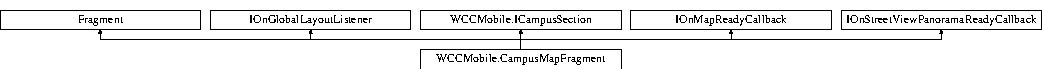
\includegraphics[height=0.921811cm]{class_w_c_c_mobile_1_1_campus_map_fragment}
\end{center}
\end{figure}
\subsection*{Public Member Functions}
\begin{DoxyCompactItemize}
\item 
\hyperlink{class_w_c_c_mobile_1_1_campus_map_fragment_ad3136fc51f47c525e00231b068431d1c}{Campus\+Map\+Fragment} ()
\begin{DoxyCompactList}\small\item\em Initializes a new instance of the \hyperlink{class_w_c_c_mobile_1_1_campus_map_fragment}{Campus\+Map\+Fragment} class. \end{DoxyCompactList}\item 
\hyperlink{class_w_c_c_mobile_1_1_campus_map_fragment_a25a52daf978a6b8e21feb51b5fbcc98c}{Campus\+Map\+Fragment} (Context context)
\begin{DoxyCompactList}\small\item\em Initializes a new instance of the \hyperlink{class_w_c_c_mobile_1_1_campus_map_fragment}{Campus\+Map\+Fragment} class. \end{DoxyCompactList}\item 
void \hyperlink{class_w_c_c_mobile_1_1_campus_map_fragment_aea93c17966750a5a7e29f7add0b29182}{Refresh\+Data} ()
\begin{DoxyCompactList}\small\item\em Refreshes the data. \end{DoxyCompactList}\item 
override void \hyperlink{class_w_c_c_mobile_1_1_campus_map_fragment_a623834901f10d1bb69af1668aa9a5e56}{On\+Activity\+Created} (Bundle saved\+Instance\+State)
\begin{DoxyCompactList}\small\item\em Called when \mbox{[}activity created\mbox{]}. \end{DoxyCompactList}\item 
override void \hyperlink{class_w_c_c_mobile_1_1_campus_map_fragment_ab8a6866347bd85d54a0c6a6fb2075ad3}{On\+Start} ()
\begin{DoxyCompactList}\small\item\em Called when \mbox{[}start\mbox{]}. \end{DoxyCompactList}\item 
void \hyperlink{class_w_c_c_mobile_1_1_campus_map_fragment_adf647c7d6ae94cdff17022cde53edbd9}{On\+Global\+Layout} ()
\begin{DoxyCompactList}\small\item\em Called when \mbox{[}global layout\mbox{]}. \end{DoxyCompactList}\item 
override View \hyperlink{class_w_c_c_mobile_1_1_campus_map_fragment_ada9727c4138ee52355e2442046846df1}{On\+Create\+View} (Layout\+Inflater inflater, View\+Group container, Bundle saved\+Instance\+State)
\begin{DoxyCompactList}\small\item\em Called when \mbox{[}create view\mbox{]}. \end{DoxyCompactList}\item 
override void \hyperlink{class_w_c_c_mobile_1_1_campus_map_fragment_a8198ceb448fd29b291533e4deb4de3d4}{On\+View\+Created} (View view, Bundle saved\+Instance\+State)
\begin{DoxyCompactList}\small\item\em Called when \mbox{[}view created\mbox{]}. \end{DoxyCompactList}\item 
void \hyperlink{class_w_c_c_mobile_1_1_campus_map_fragment_a7b89893942f57332738e6cf84cc08301}{On\+Map\+Ready} (Google\+Map google\+Map)
\begin{DoxyCompactList}\small\item\em Called when \mbox{[}map ready\mbox{]}. \end{DoxyCompactList}\item 
void \hyperlink{class_w_c_c_mobile_1_1_campus_map_fragment_aae1f4244888a3f9077a56980d45dc004}{On\+Street\+View\+Panorama\+Ready} (Street\+View\+Panorama panorama)
\begin{DoxyCompactList}\small\item\em Called when \mbox{[}street view panorama ready\mbox{]}. \end{DoxyCompactList}\item 
override void \hyperlink{class_w_c_c_mobile_1_1_campus_map_fragment_a4eb5bcf319de03bee37353f4f7418b15}{On\+Create\+Options\+Menu} (I\+Menu menu, Menu\+Inflater inflater)
\begin{DoxyCompactList}\small\item\em Called when \mbox{[}create options menu\mbox{]}. \end{DoxyCompactList}\item 
override bool \hyperlink{class_w_c_c_mobile_1_1_campus_map_fragment_a4356e19706767f8c93a1c9861492f6c7}{On\+Options\+Item\+Selected} (I\+Menu\+Item item)
\begin{DoxyCompactList}\small\item\em Called when \mbox{[}options item selected\mbox{]}. \end{DoxyCompactList}\item 
override void \hyperlink{class_w_c_c_mobile_1_1_campus_map_fragment_a2e40c56cffe4afd446324f7e6c17dbf0}{On\+View\+State\+Restored} (Bundle saved\+Instance\+State)
\begin{DoxyCompactList}\small\item\em Called when \mbox{[}view state restored\mbox{]}. \end{DoxyCompactList}\item 
override void \hyperlink{class_w_c_c_mobile_1_1_campus_map_fragment_a276a913a3425ff6fea8e2a9e1a2dceab}{On\+Resume} ()
\begin{DoxyCompactList}\small\item\em Called when \mbox{[}resume\mbox{]}. \end{DoxyCompactList}\item 
override void \hyperlink{class_w_c_c_mobile_1_1_campus_map_fragment_ac9421f08586c486240677e620e1b77f8}{On\+Low\+Memory} ()
\begin{DoxyCompactList}\small\item\em Called when \mbox{[}low memory\mbox{]}. \end{DoxyCompactList}\item 
override void \hyperlink{class_w_c_c_mobile_1_1_campus_map_fragment_ab9a654ae03b0694e2f9364daefa38a73}{On\+Pause} ()
\begin{DoxyCompactList}\small\item\em Called when \mbox{[}pause\mbox{]}. \end{DoxyCompactList}\item 
override void \hyperlink{class_w_c_c_mobile_1_1_campus_map_fragment_ae36cb06e31b5df89265c090fc793a02f}{On\+Destroy} ()
\begin{DoxyCompactList}\small\item\em Called when \mbox{[}destroy\mbox{]}. \end{DoxyCompactList}\item 
override void \hyperlink{class_w_c_c_mobile_1_1_campus_map_fragment_aba8e302e20805918185e31239ad77553}{On\+Save\+Instance\+State} (Bundle out\+State)
\begin{DoxyCompactList}\small\item\em Called when \mbox{[}save instance state\mbox{]}. \end{DoxyCompactList}\item 
async void \hyperlink{class_w_c_c_mobile_1_1_campus_map_fragment_a4ebd3585687433851b85f97b7dd7d263}{Fill\+Up\+Map} (bool force\+Refresh)
\begin{DoxyCompactList}\small\item\em Fills up map. \end{DoxyCompactList}\item 
void \hyperlink{class_w_c_c_mobile_1_1_campus_map_fragment_aa223f27f3e33ce306c48f1b046aadee3}{Center\+And\+Open\+On\+Map} (long id, float zoom=13, int anim\+Duration\+ID=Android.\+Resource.\+Integer.\+Config\+Short\+Anim\+Time)
\begin{DoxyCompactList}\small\item\em Center and open location related info on map. \end{DoxyCompactList}\item 
void \hyperlink{class_w_c_c_mobile_1_1_campus_map_fragment_a8e29f0c6d1e38218da346928adbcc219}{Center\+And\+Open\+On\+Map} (Marker marker, float zoom=13, int anim\+Duration\+ID=Android.\+Resource.\+Integer.\+Config\+Short\+Anim\+Time)
\begin{DoxyCompactList}\small\item\em Center amd open on map. \end{DoxyCompactList}\item 
void \hyperlink{class_w_c_c_mobile_1_1_campus_map_fragment_a84edd9783492a39586240f3280be9112}{Open\+Schedule\+Item\+With\+Marker} (Marker marker)
\begin{DoxyCompactList}\small\item\em Opens the schedule item with marker. \end{DoxyCompactList}\item 
void \hyperlink{class_w_c_c_mobile_1_1_campus_map_fragment_aa93bb230cabe12b3a941dc70dbeeb8c4}{Center\+Map\+On\+Location} (Lat\+Lng lat\+Lng)
\begin{DoxyCompactList}\small\item\em Centers the map on location. \end{DoxyCompactList}\item 
void \hyperlink{class_w_c_c_mobile_1_1_campus_map_fragment_aa2c1d521ebaee9cd15e437e84466a791}{On\+Search\+Intent} (Intent intent)
\begin{DoxyCompactList}\small\item\em Called when \mbox{[}search intent\mbox{]}. \end{DoxyCompactList}\end{DoxyCompactItemize}
\subsection*{Properties}
\begin{DoxyCompactItemize}
\item 
string \hyperlink{class_w_c_c_mobile_1_1_campus_map_fragment_a239196a5a923d1ac5e9d66464cb39888}{Name}\hspace{0.3cm}{\ttfamily  \mbox{[}get\mbox{]}}
\begin{DoxyCompactList}\small\item\em Gets the name. \end{DoxyCompactList}\item 
string \hyperlink{class_w_c_c_mobile_1_1_campus_map_fragment_aff146bee1b2f41f80344c3621006d833}{Title}\hspace{0.3cm}{\ttfamily  \mbox{[}get\mbox{]}}
\begin{DoxyCompactList}\small\item\em Gets the title. \end{DoxyCompactList}\end{DoxyCompactItemize}


\subsection{Constructor \& Destructor Documentation}
\index{W\+C\+C\+Mobile\+::\+Campus\+Map\+Fragment@{W\+C\+C\+Mobile\+::\+Campus\+Map\+Fragment}!Campus\+Map\+Fragment@{Campus\+Map\+Fragment}}
\index{Campus\+Map\+Fragment@{Campus\+Map\+Fragment}!W\+C\+C\+Mobile\+::\+Campus\+Map\+Fragment@{W\+C\+C\+Mobile\+::\+Campus\+Map\+Fragment}}
\subsubsection[{\texorpdfstring{Campus\+Map\+Fragment()}{CampusMapFragment()}}]{\setlength{\rightskip}{0pt plus 5cm}W\+C\+C\+Mobile.\+Campus\+Map\+Fragment.\+Campus\+Map\+Fragment (
\begin{DoxyParamCaption}
{}
\end{DoxyParamCaption}
)}\hypertarget{class_w_c_c_mobile_1_1_campus_map_fragment_ad3136fc51f47c525e00231b068431d1c}{}\label{class_w_c_c_mobile_1_1_campus_map_fragment_ad3136fc51f47c525e00231b068431d1c}


Initializes a new instance of the \hyperlink{class_w_c_c_mobile_1_1_campus_map_fragment}{Campus\+Map\+Fragment} class. 

\index{W\+C\+C\+Mobile\+::\+Campus\+Map\+Fragment@{W\+C\+C\+Mobile\+::\+Campus\+Map\+Fragment}!Campus\+Map\+Fragment@{Campus\+Map\+Fragment}}
\index{Campus\+Map\+Fragment@{Campus\+Map\+Fragment}!W\+C\+C\+Mobile\+::\+Campus\+Map\+Fragment@{W\+C\+C\+Mobile\+::\+Campus\+Map\+Fragment}}
\subsubsection[{\texorpdfstring{Campus\+Map\+Fragment(\+Context context)}{CampusMapFragment(Context context)}}]{\setlength{\rightskip}{0pt plus 5cm}W\+C\+C\+Mobile.\+Campus\+Map\+Fragment.\+Campus\+Map\+Fragment (
\begin{DoxyParamCaption}
\item[{Context}]{context}
\end{DoxyParamCaption}
)}\hypertarget{class_w_c_c_mobile_1_1_campus_map_fragment_a25a52daf978a6b8e21feb51b5fbcc98c}{}\label{class_w_c_c_mobile_1_1_campus_map_fragment_a25a52daf978a6b8e21feb51b5fbcc98c}


Initializes a new instance of the \hyperlink{class_w_c_c_mobile_1_1_campus_map_fragment}{Campus\+Map\+Fragment} class. 


\begin{DoxyParams}{Parameters}
{\em context} & The context.\\
\hline
\end{DoxyParams}


\subsection{Member Function Documentation}
\index{W\+C\+C\+Mobile\+::\+Campus\+Map\+Fragment@{W\+C\+C\+Mobile\+::\+Campus\+Map\+Fragment}!Center\+And\+Open\+On\+Map@{Center\+And\+Open\+On\+Map}}
\index{Center\+And\+Open\+On\+Map@{Center\+And\+Open\+On\+Map}!W\+C\+C\+Mobile\+::\+Campus\+Map\+Fragment@{W\+C\+C\+Mobile\+::\+Campus\+Map\+Fragment}}
\subsubsection[{\texorpdfstring{Center\+And\+Open\+On\+Map(long id, float zoom=13, int anim\+Duration\+I\+D=\+Android.\+Resource.\+Integer.\+Config\+Short\+Anim\+Time)}{CenterAndOpenOnMap(long id, float zoom=13, int animDurationID=Android.Resource.Integer.ConfigShortAnimTime)}}]{\setlength{\rightskip}{0pt plus 5cm}void W\+C\+C\+Mobile.\+Campus\+Map\+Fragment.\+Center\+And\+Open\+On\+Map (
\begin{DoxyParamCaption}
\item[{long}]{id, }
\item[{float}]{zoom = {\ttfamily 13}, }
\item[{int}]{anim\+Duration\+ID = {\ttfamily Android.Resource.Integer.ConfigShortAnimTime}}
\end{DoxyParamCaption}
)}\hypertarget{class_w_c_c_mobile_1_1_campus_map_fragment_aa223f27f3e33ce306c48f1b046aadee3}{}\label{class_w_c_c_mobile_1_1_campus_map_fragment_aa223f27f3e33ce306c48f1b046aadee3}


Center and open location related info on map. 


\begin{DoxyParams}{Parameters}
{\em id} & The identifier.\\
\hline
{\em zoom} & The zoom.\\
\hline
{\em anim\+Duration\+ID} & The anim duration identifier.\\
\hline
\end{DoxyParams}
\index{W\+C\+C\+Mobile\+::\+Campus\+Map\+Fragment@{W\+C\+C\+Mobile\+::\+Campus\+Map\+Fragment}!Center\+And\+Open\+On\+Map@{Center\+And\+Open\+On\+Map}}
\index{Center\+And\+Open\+On\+Map@{Center\+And\+Open\+On\+Map}!W\+C\+C\+Mobile\+::\+Campus\+Map\+Fragment@{W\+C\+C\+Mobile\+::\+Campus\+Map\+Fragment}}
\subsubsection[{\texorpdfstring{Center\+And\+Open\+On\+Map(\+Marker marker, float zoom=13, int anim\+Duration\+I\+D=\+Android.\+Resource.\+Integer.\+Config\+Short\+Anim\+Time)}{CenterAndOpenOnMap(Marker marker, float zoom=13, int animDurationID=Android.Resource.Integer.ConfigShortAnimTime)}}]{\setlength{\rightskip}{0pt plus 5cm}void W\+C\+C\+Mobile.\+Campus\+Map\+Fragment.\+Center\+And\+Open\+On\+Map (
\begin{DoxyParamCaption}
\item[{Marker}]{marker, }
\item[{float}]{zoom = {\ttfamily 13}, }
\item[{int}]{anim\+Duration\+ID = {\ttfamily Android.Resource.Integer.ConfigShortAnimTime}}
\end{DoxyParamCaption}
)}\hypertarget{class_w_c_c_mobile_1_1_campus_map_fragment_a8e29f0c6d1e38218da346928adbcc219}{}\label{class_w_c_c_mobile_1_1_campus_map_fragment_a8e29f0c6d1e38218da346928adbcc219}


Center amd open on map. 


\begin{DoxyParams}{Parameters}
{\em marker} & The marker.\\
\hline
{\em zoom} & The zoom.\\
\hline
{\em anim\+Duration\+ID} & The anim duration identifier.\\
\hline
\end{DoxyParams}
\index{W\+C\+C\+Mobile\+::\+Campus\+Map\+Fragment@{W\+C\+C\+Mobile\+::\+Campus\+Map\+Fragment}!Center\+Map\+On\+Location@{Center\+Map\+On\+Location}}
\index{Center\+Map\+On\+Location@{Center\+Map\+On\+Location}!W\+C\+C\+Mobile\+::\+Campus\+Map\+Fragment@{W\+C\+C\+Mobile\+::\+Campus\+Map\+Fragment}}
\subsubsection[{\texorpdfstring{Center\+Map\+On\+Location(\+Lat\+Lng lat\+Lng)}{CenterMapOnLocation(LatLng latLng)}}]{\setlength{\rightskip}{0pt plus 5cm}void W\+C\+C\+Mobile.\+Campus\+Map\+Fragment.\+Center\+Map\+On\+Location (
\begin{DoxyParamCaption}
\item[{Lat\+Lng}]{lat\+Lng}
\end{DoxyParamCaption}
)}\hypertarget{class_w_c_c_mobile_1_1_campus_map_fragment_aa93bb230cabe12b3a941dc70dbeeb8c4}{}\label{class_w_c_c_mobile_1_1_campus_map_fragment_aa93bb230cabe12b3a941dc70dbeeb8c4}


Centers the map on location. 


\begin{DoxyParams}{Parameters}
{\em lat\+Lng} & The lat L\+NG.\\
\hline
\end{DoxyParams}
\index{W\+C\+C\+Mobile\+::\+Campus\+Map\+Fragment@{W\+C\+C\+Mobile\+::\+Campus\+Map\+Fragment}!Fill\+Up\+Map@{Fill\+Up\+Map}}
\index{Fill\+Up\+Map@{Fill\+Up\+Map}!W\+C\+C\+Mobile\+::\+Campus\+Map\+Fragment@{W\+C\+C\+Mobile\+::\+Campus\+Map\+Fragment}}
\subsubsection[{\texorpdfstring{Fill\+Up\+Map(bool force\+Refresh)}{FillUpMap(bool forceRefresh)}}]{\setlength{\rightskip}{0pt plus 5cm}async void W\+C\+C\+Mobile.\+Campus\+Map\+Fragment.\+Fill\+Up\+Map (
\begin{DoxyParamCaption}
\item[{bool}]{force\+Refresh}
\end{DoxyParamCaption}
)}\hypertarget{class_w_c_c_mobile_1_1_campus_map_fragment_a4ebd3585687433851b85f97b7dd7d263}{}\label{class_w_c_c_mobile_1_1_campus_map_fragment_a4ebd3585687433851b85f97b7dd7d263}


Fills up map. 


\begin{DoxyParams}{Parameters}
{\em force\+Refresh} & if set to {\ttfamily true} \mbox{[}force refresh\mbox{]}.\\
\hline
\end{DoxyParams}
\index{W\+C\+C\+Mobile\+::\+Campus\+Map\+Fragment@{W\+C\+C\+Mobile\+::\+Campus\+Map\+Fragment}!On\+Activity\+Created@{On\+Activity\+Created}}
\index{On\+Activity\+Created@{On\+Activity\+Created}!W\+C\+C\+Mobile\+::\+Campus\+Map\+Fragment@{W\+C\+C\+Mobile\+::\+Campus\+Map\+Fragment}}
\subsubsection[{\texorpdfstring{On\+Activity\+Created(\+Bundle saved\+Instance\+State)}{OnActivityCreated(Bundle savedInstanceState)}}]{\setlength{\rightskip}{0pt plus 5cm}override void W\+C\+C\+Mobile.\+Campus\+Map\+Fragment.\+On\+Activity\+Created (
\begin{DoxyParamCaption}
\item[{Bundle}]{saved\+Instance\+State}
\end{DoxyParamCaption}
)}\hypertarget{class_w_c_c_mobile_1_1_campus_map_fragment_a623834901f10d1bb69af1668aa9a5e56}{}\label{class_w_c_c_mobile_1_1_campus_map_fragment_a623834901f10d1bb69af1668aa9a5e56}


Called when \mbox{[}activity created\mbox{]}. 


\begin{DoxyParams}{Parameters}
{\em saved\+Instance\+State} & State of the saved instance.\\
\hline
\end{DoxyParams}
\index{W\+C\+C\+Mobile\+::\+Campus\+Map\+Fragment@{W\+C\+C\+Mobile\+::\+Campus\+Map\+Fragment}!On\+Create\+Options\+Menu@{On\+Create\+Options\+Menu}}
\index{On\+Create\+Options\+Menu@{On\+Create\+Options\+Menu}!W\+C\+C\+Mobile\+::\+Campus\+Map\+Fragment@{W\+C\+C\+Mobile\+::\+Campus\+Map\+Fragment}}
\subsubsection[{\texorpdfstring{On\+Create\+Options\+Menu(\+I\+Menu menu, Menu\+Inflater inflater)}{OnCreateOptionsMenu(IMenu menu, MenuInflater inflater)}}]{\setlength{\rightskip}{0pt plus 5cm}override void W\+C\+C\+Mobile.\+Campus\+Map\+Fragment.\+On\+Create\+Options\+Menu (
\begin{DoxyParamCaption}
\item[{I\+Menu}]{menu, }
\item[{Menu\+Inflater}]{inflater}
\end{DoxyParamCaption}
)}\hypertarget{class_w_c_c_mobile_1_1_campus_map_fragment_a4eb5bcf319de03bee37353f4f7418b15}{}\label{class_w_c_c_mobile_1_1_campus_map_fragment_a4eb5bcf319de03bee37353f4f7418b15}


Called when \mbox{[}create options menu\mbox{]}. 


\begin{DoxyParams}{Parameters}
{\em menu} & The menu.\\
\hline
{\em inflater} & The inflater.\\
\hline
\end{DoxyParams}
\index{W\+C\+C\+Mobile\+::\+Campus\+Map\+Fragment@{W\+C\+C\+Mobile\+::\+Campus\+Map\+Fragment}!On\+Create\+View@{On\+Create\+View}}
\index{On\+Create\+View@{On\+Create\+View}!W\+C\+C\+Mobile\+::\+Campus\+Map\+Fragment@{W\+C\+C\+Mobile\+::\+Campus\+Map\+Fragment}}
\subsubsection[{\texorpdfstring{On\+Create\+View(\+Layout\+Inflater inflater, View\+Group container, Bundle saved\+Instance\+State)}{OnCreateView(LayoutInflater inflater, ViewGroup container, Bundle savedInstanceState)}}]{\setlength{\rightskip}{0pt plus 5cm}override View W\+C\+C\+Mobile.\+Campus\+Map\+Fragment.\+On\+Create\+View (
\begin{DoxyParamCaption}
\item[{Layout\+Inflater}]{inflater, }
\item[{View\+Group}]{container, }
\item[{Bundle}]{saved\+Instance\+State}
\end{DoxyParamCaption}
)}\hypertarget{class_w_c_c_mobile_1_1_campus_map_fragment_ada9727c4138ee52355e2442046846df1}{}\label{class_w_c_c_mobile_1_1_campus_map_fragment_ada9727c4138ee52355e2442046846df1}


Called when \mbox{[}create view\mbox{]}. 


\begin{DoxyParams}{Parameters}
{\em inflater} & The inflater.\\
\hline
{\em container} & The container.\\
\hline
{\em saved\+Instance\+State} & State of the saved instance.\\
\hline
\end{DoxyParams}
\begin{DoxyReturn}{Returns}

\end{DoxyReturn}
\index{W\+C\+C\+Mobile\+::\+Campus\+Map\+Fragment@{W\+C\+C\+Mobile\+::\+Campus\+Map\+Fragment}!On\+Destroy@{On\+Destroy}}
\index{On\+Destroy@{On\+Destroy}!W\+C\+C\+Mobile\+::\+Campus\+Map\+Fragment@{W\+C\+C\+Mobile\+::\+Campus\+Map\+Fragment}}
\subsubsection[{\texorpdfstring{On\+Destroy()}{OnDestroy()}}]{\setlength{\rightskip}{0pt plus 5cm}override void W\+C\+C\+Mobile.\+Campus\+Map\+Fragment.\+On\+Destroy (
\begin{DoxyParamCaption}
{}
\end{DoxyParamCaption}
)}\hypertarget{class_w_c_c_mobile_1_1_campus_map_fragment_ae36cb06e31b5df89265c090fc793a02f}{}\label{class_w_c_c_mobile_1_1_campus_map_fragment_ae36cb06e31b5df89265c090fc793a02f}


Called when \mbox{[}destroy\mbox{]}. 

\index{W\+C\+C\+Mobile\+::\+Campus\+Map\+Fragment@{W\+C\+C\+Mobile\+::\+Campus\+Map\+Fragment}!On\+Global\+Layout@{On\+Global\+Layout}}
\index{On\+Global\+Layout@{On\+Global\+Layout}!W\+C\+C\+Mobile\+::\+Campus\+Map\+Fragment@{W\+C\+C\+Mobile\+::\+Campus\+Map\+Fragment}}
\subsubsection[{\texorpdfstring{On\+Global\+Layout()}{OnGlobalLayout()}}]{\setlength{\rightskip}{0pt plus 5cm}void W\+C\+C\+Mobile.\+Campus\+Map\+Fragment.\+On\+Global\+Layout (
\begin{DoxyParamCaption}
{}
\end{DoxyParamCaption}
)}\hypertarget{class_w_c_c_mobile_1_1_campus_map_fragment_adf647c7d6ae94cdff17022cde53edbd9}{}\label{class_w_c_c_mobile_1_1_campus_map_fragment_adf647c7d6ae94cdff17022cde53edbd9}


Called when \mbox{[}global layout\mbox{]}. 

\index{W\+C\+C\+Mobile\+::\+Campus\+Map\+Fragment@{W\+C\+C\+Mobile\+::\+Campus\+Map\+Fragment}!On\+Low\+Memory@{On\+Low\+Memory}}
\index{On\+Low\+Memory@{On\+Low\+Memory}!W\+C\+C\+Mobile\+::\+Campus\+Map\+Fragment@{W\+C\+C\+Mobile\+::\+Campus\+Map\+Fragment}}
\subsubsection[{\texorpdfstring{On\+Low\+Memory()}{OnLowMemory()}}]{\setlength{\rightskip}{0pt plus 5cm}override void W\+C\+C\+Mobile.\+Campus\+Map\+Fragment.\+On\+Low\+Memory (
\begin{DoxyParamCaption}
{}
\end{DoxyParamCaption}
)}\hypertarget{class_w_c_c_mobile_1_1_campus_map_fragment_ac9421f08586c486240677e620e1b77f8}{}\label{class_w_c_c_mobile_1_1_campus_map_fragment_ac9421f08586c486240677e620e1b77f8}


Called when \mbox{[}low memory\mbox{]}. 

\index{W\+C\+C\+Mobile\+::\+Campus\+Map\+Fragment@{W\+C\+C\+Mobile\+::\+Campus\+Map\+Fragment}!On\+Map\+Ready@{On\+Map\+Ready}}
\index{On\+Map\+Ready@{On\+Map\+Ready}!W\+C\+C\+Mobile\+::\+Campus\+Map\+Fragment@{W\+C\+C\+Mobile\+::\+Campus\+Map\+Fragment}}
\subsubsection[{\texorpdfstring{On\+Map\+Ready(\+Google\+Map google\+Map)}{OnMapReady(GoogleMap googleMap)}}]{\setlength{\rightskip}{0pt plus 5cm}void W\+C\+C\+Mobile.\+Campus\+Map\+Fragment.\+On\+Map\+Ready (
\begin{DoxyParamCaption}
\item[{Google\+Map}]{google\+Map}
\end{DoxyParamCaption}
)}\hypertarget{class_w_c_c_mobile_1_1_campus_map_fragment_a7b89893942f57332738e6cf84cc08301}{}\label{class_w_c_c_mobile_1_1_campus_map_fragment_a7b89893942f57332738e6cf84cc08301}


Called when \mbox{[}map ready\mbox{]}. 


\begin{DoxyParams}{Parameters}
{\em google\+Map} & The google map.\\
\hline
\end{DoxyParams}
\index{W\+C\+C\+Mobile\+::\+Campus\+Map\+Fragment@{W\+C\+C\+Mobile\+::\+Campus\+Map\+Fragment}!On\+Options\+Item\+Selected@{On\+Options\+Item\+Selected}}
\index{On\+Options\+Item\+Selected@{On\+Options\+Item\+Selected}!W\+C\+C\+Mobile\+::\+Campus\+Map\+Fragment@{W\+C\+C\+Mobile\+::\+Campus\+Map\+Fragment}}
\subsubsection[{\texorpdfstring{On\+Options\+Item\+Selected(\+I\+Menu\+Item item)}{OnOptionsItemSelected(IMenuItem item)}}]{\setlength{\rightskip}{0pt plus 5cm}override bool W\+C\+C\+Mobile.\+Campus\+Map\+Fragment.\+On\+Options\+Item\+Selected (
\begin{DoxyParamCaption}
\item[{I\+Menu\+Item}]{item}
\end{DoxyParamCaption}
)}\hypertarget{class_w_c_c_mobile_1_1_campus_map_fragment_a4356e19706767f8c93a1c9861492f6c7}{}\label{class_w_c_c_mobile_1_1_campus_map_fragment_a4356e19706767f8c93a1c9861492f6c7}


Called when \mbox{[}options item selected\mbox{]}. 


\begin{DoxyParams}{Parameters}
{\em item} & The item.\\
\hline
\end{DoxyParams}
\begin{DoxyReturn}{Returns}

\end{DoxyReturn}
\index{W\+C\+C\+Mobile\+::\+Campus\+Map\+Fragment@{W\+C\+C\+Mobile\+::\+Campus\+Map\+Fragment}!On\+Pause@{On\+Pause}}
\index{On\+Pause@{On\+Pause}!W\+C\+C\+Mobile\+::\+Campus\+Map\+Fragment@{W\+C\+C\+Mobile\+::\+Campus\+Map\+Fragment}}
\subsubsection[{\texorpdfstring{On\+Pause()}{OnPause()}}]{\setlength{\rightskip}{0pt plus 5cm}override void W\+C\+C\+Mobile.\+Campus\+Map\+Fragment.\+On\+Pause (
\begin{DoxyParamCaption}
{}
\end{DoxyParamCaption}
)}\hypertarget{class_w_c_c_mobile_1_1_campus_map_fragment_ab9a654ae03b0694e2f9364daefa38a73}{}\label{class_w_c_c_mobile_1_1_campus_map_fragment_ab9a654ae03b0694e2f9364daefa38a73}


Called when \mbox{[}pause\mbox{]}. 

\index{W\+C\+C\+Mobile\+::\+Campus\+Map\+Fragment@{W\+C\+C\+Mobile\+::\+Campus\+Map\+Fragment}!On\+Resume@{On\+Resume}}
\index{On\+Resume@{On\+Resume}!W\+C\+C\+Mobile\+::\+Campus\+Map\+Fragment@{W\+C\+C\+Mobile\+::\+Campus\+Map\+Fragment}}
\subsubsection[{\texorpdfstring{On\+Resume()}{OnResume()}}]{\setlength{\rightskip}{0pt plus 5cm}override void W\+C\+C\+Mobile.\+Campus\+Map\+Fragment.\+On\+Resume (
\begin{DoxyParamCaption}
{}
\end{DoxyParamCaption}
)}\hypertarget{class_w_c_c_mobile_1_1_campus_map_fragment_a276a913a3425ff6fea8e2a9e1a2dceab}{}\label{class_w_c_c_mobile_1_1_campus_map_fragment_a276a913a3425ff6fea8e2a9e1a2dceab}


Called when \mbox{[}resume\mbox{]}. 

\index{W\+C\+C\+Mobile\+::\+Campus\+Map\+Fragment@{W\+C\+C\+Mobile\+::\+Campus\+Map\+Fragment}!On\+Save\+Instance\+State@{On\+Save\+Instance\+State}}
\index{On\+Save\+Instance\+State@{On\+Save\+Instance\+State}!W\+C\+C\+Mobile\+::\+Campus\+Map\+Fragment@{W\+C\+C\+Mobile\+::\+Campus\+Map\+Fragment}}
\subsubsection[{\texorpdfstring{On\+Save\+Instance\+State(\+Bundle out\+State)}{OnSaveInstanceState(Bundle outState)}}]{\setlength{\rightskip}{0pt plus 5cm}override void W\+C\+C\+Mobile.\+Campus\+Map\+Fragment.\+On\+Save\+Instance\+State (
\begin{DoxyParamCaption}
\item[{Bundle}]{out\+State}
\end{DoxyParamCaption}
)}\hypertarget{class_w_c_c_mobile_1_1_campus_map_fragment_aba8e302e20805918185e31239ad77553}{}\label{class_w_c_c_mobile_1_1_campus_map_fragment_aba8e302e20805918185e31239ad77553}


Called when \mbox{[}save instance state\mbox{]}. 


\begin{DoxyParams}{Parameters}
{\em out\+State} & State of the out.\\
\hline
\end{DoxyParams}
\index{W\+C\+C\+Mobile\+::\+Campus\+Map\+Fragment@{W\+C\+C\+Mobile\+::\+Campus\+Map\+Fragment}!On\+Search\+Intent@{On\+Search\+Intent}}
\index{On\+Search\+Intent@{On\+Search\+Intent}!W\+C\+C\+Mobile\+::\+Campus\+Map\+Fragment@{W\+C\+C\+Mobile\+::\+Campus\+Map\+Fragment}}
\subsubsection[{\texorpdfstring{On\+Search\+Intent(\+Intent intent)}{OnSearchIntent(Intent intent)}}]{\setlength{\rightskip}{0pt plus 5cm}void W\+C\+C\+Mobile.\+Campus\+Map\+Fragment.\+On\+Search\+Intent (
\begin{DoxyParamCaption}
\item[{Intent}]{intent}
\end{DoxyParamCaption}
)}\hypertarget{class_w_c_c_mobile_1_1_campus_map_fragment_aa2c1d521ebaee9cd15e437e84466a791}{}\label{class_w_c_c_mobile_1_1_campus_map_fragment_aa2c1d521ebaee9cd15e437e84466a791}


Called when \mbox{[}search intent\mbox{]}. 


\begin{DoxyParams}{Parameters}
{\em intent} & The intent.\\
\hline
\end{DoxyParams}
\index{W\+C\+C\+Mobile\+::\+Campus\+Map\+Fragment@{W\+C\+C\+Mobile\+::\+Campus\+Map\+Fragment}!On\+Start@{On\+Start}}
\index{On\+Start@{On\+Start}!W\+C\+C\+Mobile\+::\+Campus\+Map\+Fragment@{W\+C\+C\+Mobile\+::\+Campus\+Map\+Fragment}}
\subsubsection[{\texorpdfstring{On\+Start()}{OnStart()}}]{\setlength{\rightskip}{0pt plus 5cm}override void W\+C\+C\+Mobile.\+Campus\+Map\+Fragment.\+On\+Start (
\begin{DoxyParamCaption}
{}
\end{DoxyParamCaption}
)}\hypertarget{class_w_c_c_mobile_1_1_campus_map_fragment_ab8a6866347bd85d54a0c6a6fb2075ad3}{}\label{class_w_c_c_mobile_1_1_campus_map_fragment_ab8a6866347bd85d54a0c6a6fb2075ad3}


Called when \mbox{[}start\mbox{]}. 

\index{W\+C\+C\+Mobile\+::\+Campus\+Map\+Fragment@{W\+C\+C\+Mobile\+::\+Campus\+Map\+Fragment}!On\+Street\+View\+Panorama\+Ready@{On\+Street\+View\+Panorama\+Ready}}
\index{On\+Street\+View\+Panorama\+Ready@{On\+Street\+View\+Panorama\+Ready}!W\+C\+C\+Mobile\+::\+Campus\+Map\+Fragment@{W\+C\+C\+Mobile\+::\+Campus\+Map\+Fragment}}
\subsubsection[{\texorpdfstring{On\+Street\+View\+Panorama\+Ready(\+Street\+View\+Panorama panorama)}{OnStreetViewPanoramaReady(StreetViewPanorama panorama)}}]{\setlength{\rightskip}{0pt plus 5cm}void W\+C\+C\+Mobile.\+Campus\+Map\+Fragment.\+On\+Street\+View\+Panorama\+Ready (
\begin{DoxyParamCaption}
\item[{Street\+View\+Panorama}]{panorama}
\end{DoxyParamCaption}
)}\hypertarget{class_w_c_c_mobile_1_1_campus_map_fragment_aae1f4244888a3f9077a56980d45dc004}{}\label{class_w_c_c_mobile_1_1_campus_map_fragment_aae1f4244888a3f9077a56980d45dc004}


Called when \mbox{[}street view panorama ready\mbox{]}. 


\begin{DoxyParams}{Parameters}
{\em panorama} & The panorama.\\
\hline
\end{DoxyParams}
\index{W\+C\+C\+Mobile\+::\+Campus\+Map\+Fragment@{W\+C\+C\+Mobile\+::\+Campus\+Map\+Fragment}!On\+View\+Created@{On\+View\+Created}}
\index{On\+View\+Created@{On\+View\+Created}!W\+C\+C\+Mobile\+::\+Campus\+Map\+Fragment@{W\+C\+C\+Mobile\+::\+Campus\+Map\+Fragment}}
\subsubsection[{\texorpdfstring{On\+View\+Created(\+View view, Bundle saved\+Instance\+State)}{OnViewCreated(View view, Bundle savedInstanceState)}}]{\setlength{\rightskip}{0pt plus 5cm}override void W\+C\+C\+Mobile.\+Campus\+Map\+Fragment.\+On\+View\+Created (
\begin{DoxyParamCaption}
\item[{View}]{view, }
\item[{Bundle}]{saved\+Instance\+State}
\end{DoxyParamCaption}
)}\hypertarget{class_w_c_c_mobile_1_1_campus_map_fragment_a8198ceb448fd29b291533e4deb4de3d4}{}\label{class_w_c_c_mobile_1_1_campus_map_fragment_a8198ceb448fd29b291533e4deb4de3d4}


Called when \mbox{[}view created\mbox{]}. 


\begin{DoxyParams}{Parameters}
{\em view} & The view.\\
\hline
{\em saved\+Instance\+State} & State of the saved instance.\\
\hline
\end{DoxyParams}
\index{W\+C\+C\+Mobile\+::\+Campus\+Map\+Fragment@{W\+C\+C\+Mobile\+::\+Campus\+Map\+Fragment}!On\+View\+State\+Restored@{On\+View\+State\+Restored}}
\index{On\+View\+State\+Restored@{On\+View\+State\+Restored}!W\+C\+C\+Mobile\+::\+Campus\+Map\+Fragment@{W\+C\+C\+Mobile\+::\+Campus\+Map\+Fragment}}
\subsubsection[{\texorpdfstring{On\+View\+State\+Restored(\+Bundle saved\+Instance\+State)}{OnViewStateRestored(Bundle savedInstanceState)}}]{\setlength{\rightskip}{0pt plus 5cm}override void W\+C\+C\+Mobile.\+Campus\+Map\+Fragment.\+On\+View\+State\+Restored (
\begin{DoxyParamCaption}
\item[{Bundle}]{saved\+Instance\+State}
\end{DoxyParamCaption}
)}\hypertarget{class_w_c_c_mobile_1_1_campus_map_fragment_a2e40c56cffe4afd446324f7e6c17dbf0}{}\label{class_w_c_c_mobile_1_1_campus_map_fragment_a2e40c56cffe4afd446324f7e6c17dbf0}


Called when \mbox{[}view state restored\mbox{]}. 


\begin{DoxyParams}{Parameters}
{\em saved\+Instance\+State} & State of the saved instance.\\
\hline
\end{DoxyParams}
\index{W\+C\+C\+Mobile\+::\+Campus\+Map\+Fragment@{W\+C\+C\+Mobile\+::\+Campus\+Map\+Fragment}!Open\+Schedule\+Item\+With\+Marker@{Open\+Schedule\+Item\+With\+Marker}}
\index{Open\+Schedule\+Item\+With\+Marker@{Open\+Schedule\+Item\+With\+Marker}!W\+C\+C\+Mobile\+::\+Campus\+Map\+Fragment@{W\+C\+C\+Mobile\+::\+Campus\+Map\+Fragment}}
\subsubsection[{\texorpdfstring{Open\+Schedule\+Item\+With\+Marker(\+Marker marker)}{OpenScheduleItemWithMarker(Marker marker)}}]{\setlength{\rightskip}{0pt plus 5cm}void W\+C\+C\+Mobile.\+Campus\+Map\+Fragment.\+Open\+Schedule\+Item\+With\+Marker (
\begin{DoxyParamCaption}
\item[{Marker}]{marker}
\end{DoxyParamCaption}
)}\hypertarget{class_w_c_c_mobile_1_1_campus_map_fragment_a84edd9783492a39586240f3280be9112}{}\label{class_w_c_c_mobile_1_1_campus_map_fragment_a84edd9783492a39586240f3280be9112}


Opens the schedule item with marker. 


\begin{DoxyParams}{Parameters}
{\em marker} & The marker.\\
\hline
\end{DoxyParams}
\index{W\+C\+C\+Mobile\+::\+Campus\+Map\+Fragment@{W\+C\+C\+Mobile\+::\+Campus\+Map\+Fragment}!Refresh\+Data@{Refresh\+Data}}
\index{Refresh\+Data@{Refresh\+Data}!W\+C\+C\+Mobile\+::\+Campus\+Map\+Fragment@{W\+C\+C\+Mobile\+::\+Campus\+Map\+Fragment}}
\subsubsection[{\texorpdfstring{Refresh\+Data()}{RefreshData()}}]{\setlength{\rightskip}{0pt plus 5cm}void W\+C\+C\+Mobile.\+Campus\+Map\+Fragment.\+Refresh\+Data (
\begin{DoxyParamCaption}
{}
\end{DoxyParamCaption}
)}\hypertarget{class_w_c_c_mobile_1_1_campus_map_fragment_aea93c17966750a5a7e29f7add0b29182}{}\label{class_w_c_c_mobile_1_1_campus_map_fragment_aea93c17966750a5a7e29f7add0b29182}


Refreshes the data. 



Implements \hyperlink{interface_w_c_c_mobile_1_1_i_campus_section}{W\+C\+C\+Mobile.\+I\+Campus\+Section}.



\subsection{Property Documentation}
\index{W\+C\+C\+Mobile\+::\+Campus\+Map\+Fragment@{W\+C\+C\+Mobile\+::\+Campus\+Map\+Fragment}!Name@{Name}}
\index{Name@{Name}!W\+C\+C\+Mobile\+::\+Campus\+Map\+Fragment@{W\+C\+C\+Mobile\+::\+Campus\+Map\+Fragment}}
\subsubsection[{\texorpdfstring{Name}{Name}}]{\setlength{\rightskip}{0pt plus 5cm}string W\+C\+C\+Mobile.\+Campus\+Map\+Fragment.\+Name\hspace{0.3cm}{\ttfamily [get]}}\hypertarget{class_w_c_c_mobile_1_1_campus_map_fragment_a239196a5a923d1ac5e9d66464cb39888}{}\label{class_w_c_c_mobile_1_1_campus_map_fragment_a239196a5a923d1ac5e9d66464cb39888}


Gets the name. 

The name. \index{W\+C\+C\+Mobile\+::\+Campus\+Map\+Fragment@{W\+C\+C\+Mobile\+::\+Campus\+Map\+Fragment}!Title@{Title}}
\index{Title@{Title}!W\+C\+C\+Mobile\+::\+Campus\+Map\+Fragment@{W\+C\+C\+Mobile\+::\+Campus\+Map\+Fragment}}
\subsubsection[{\texorpdfstring{Title}{Title}}]{\setlength{\rightskip}{0pt plus 5cm}string W\+C\+C\+Mobile.\+Campus\+Map\+Fragment.\+Title\hspace{0.3cm}{\ttfamily [get]}}\hypertarget{class_w_c_c_mobile_1_1_campus_map_fragment_aff146bee1b2f41f80344c3621006d833}{}\label{class_w_c_c_mobile_1_1_campus_map_fragment_aff146bee1b2f41f80344c3621006d833}


Gets the title. 

The title. 

The documentation for this class was generated from the following file\+:\begin{DoxyCompactItemize}
\item 
Source/\+Fragments/Campus\+Map\+Fragment.\+cs\end{DoxyCompactItemize}

\hypertarget{class_w_c_c_mobile_1_1_contacts_actvity}{}\section{W\+C\+C\+Mobile.\+Contacts\+Actvity Class Reference}
\label{class_w_c_c_mobile_1_1_contacts_actvity}\index{W\+C\+C\+Mobile.\+Contacts\+Actvity@{W\+C\+C\+Mobile.\+Contacts\+Actvity}}
Inheritance diagram for W\+C\+C\+Mobile.\+Contacts\+Actvity\+:\begin{figure}[H]
\begin{center}
\leavevmode
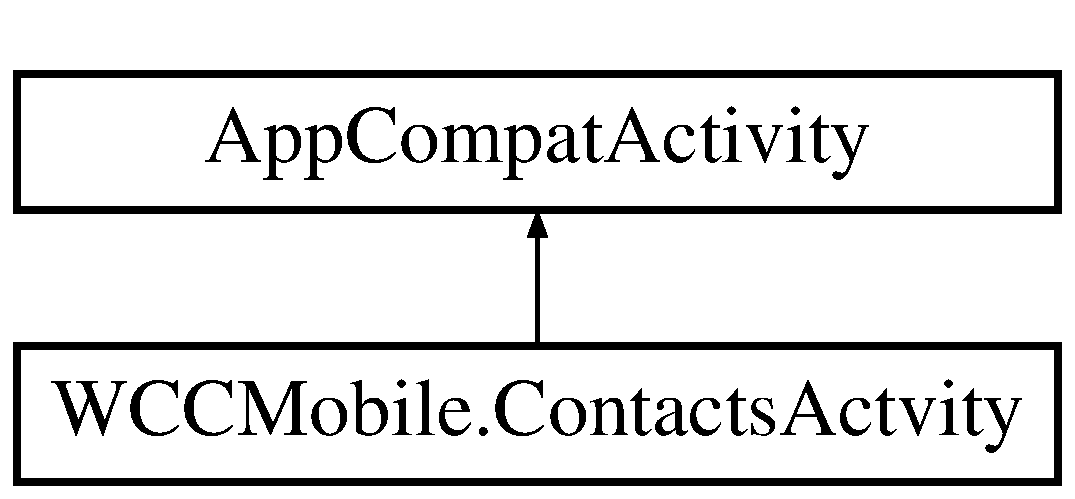
\includegraphics[height=2.000000cm]{class_w_c_c_mobile_1_1_contacts_actvity}
\end{center}
\end{figure}
\subsection*{Public Member Functions}
\begin{DoxyCompactItemize}
\item 
override void \hyperlink{class_w_c_c_mobile_1_1_contacts_actvity_a26bf3f5f6f12d20de073e2c66b808635}{On\+Back\+Pressed} ()
\begin{DoxyCompactList}\small\item\em Called when the activity has detected the user\textquotesingle{}s press of the back key. \end{DoxyCompactList}\end{DoxyCompactItemize}
\subsection*{Static Public Member Functions}
\begin{DoxyCompactItemize}
\item 
static void \hyperlink{class_w_c_c_mobile_1_1_contacts_actvity_a23ad5907d321ef68cc2d4ffe1bb8d1ee}{Call\+Number} (int Phone\+Key, Activity Caller)
\begin{DoxyCompactList}\small\item\em Function to call numbers from Yellow\+Book.\+txt -\/ Any Activity can call this function provided they pass themselves and the key to the number in the book \end{DoxyCompactList}\item 
static void \hyperlink{class_w_c_c_mobile_1_1_contacts_actvity_af752661848689d2b5c4375d132fc9121}{Send\+Email} (int Email\+Key, Activity Mailer)
\begin{DoxyCompactList}\small\item\em Method to send emails to address listed in Yellow\+Book.\+txt -\/ Any Activity can call this method provided they pass themselves and the key to the address in the book \end{DoxyCompactList}\item 
static void \hyperlink{class_w_c_c_mobile_1_1_contacts_actvity_a6c30b1b39fbee4678d39606ccb8abe0e}{Alert\+Contact} (int Phone\+Key, Activity Caller)
\begin{DoxyCompactList}\small\item\em Launches an alert with two buttons. Button 1 -\/ Phone Contact Button 2 -\/ Email Contact \end{DoxyCompactList}\end{DoxyCompactItemize}
\subsection*{Protected Member Functions}
\begin{DoxyCompactItemize}
\item 
override void \hyperlink{class_w_c_c_mobile_1_1_contacts_actvity_a2e7c8c223ecc577fc737a54cf69576d0}{On\+Create} (Bundle saved\+Instance\+State)
\begin{DoxyCompactList}\small\item\em Called when \mbox{[}create\mbox{]}. \end{DoxyCompactList}\end{DoxyCompactItemize}


\subsection{Member Function Documentation}
\index{W\+C\+C\+Mobile\+::\+Contacts\+Actvity@{W\+C\+C\+Mobile\+::\+Contacts\+Actvity}!Alert\+Contact@{Alert\+Contact}}
\index{Alert\+Contact@{Alert\+Contact}!W\+C\+C\+Mobile\+::\+Contacts\+Actvity@{W\+C\+C\+Mobile\+::\+Contacts\+Actvity}}
\subsubsection[{\texorpdfstring{Alert\+Contact(int Phone\+Key, Activity Caller)}{AlertContact(int PhoneKey, Activity Caller)}}]{\setlength{\rightskip}{0pt plus 5cm}static void W\+C\+C\+Mobile.\+Contacts\+Actvity.\+Alert\+Contact (
\begin{DoxyParamCaption}
\item[{int}]{Phone\+Key, }
\item[{Activity}]{Caller}
\end{DoxyParamCaption}
)\hspace{0.3cm}{\ttfamily [static]}}\hypertarget{class_w_c_c_mobile_1_1_contacts_actvity_a6c30b1b39fbee4678d39606ccb8abe0e}{}\label{class_w_c_c_mobile_1_1_contacts_actvity_a6c30b1b39fbee4678d39606ccb8abe0e}


Launches an alert with two buttons. Button 1 -\/ Phone Contact Button 2 -\/ Email Contact 


\begin{DoxyParams}{Parameters}
{\em Phone\+Key} & The phone key.\\
\hline
{\em Caller} & The caller.\\
\hline
\end{DoxyParams}
\index{W\+C\+C\+Mobile\+::\+Contacts\+Actvity@{W\+C\+C\+Mobile\+::\+Contacts\+Actvity}!Call\+Number@{Call\+Number}}
\index{Call\+Number@{Call\+Number}!W\+C\+C\+Mobile\+::\+Contacts\+Actvity@{W\+C\+C\+Mobile\+::\+Contacts\+Actvity}}
\subsubsection[{\texorpdfstring{Call\+Number(int Phone\+Key, Activity Caller)}{CallNumber(int PhoneKey, Activity Caller)}}]{\setlength{\rightskip}{0pt plus 5cm}static void W\+C\+C\+Mobile.\+Contacts\+Actvity.\+Call\+Number (
\begin{DoxyParamCaption}
\item[{int}]{Phone\+Key, }
\item[{Activity}]{Caller}
\end{DoxyParamCaption}
)\hspace{0.3cm}{\ttfamily [static]}}\hypertarget{class_w_c_c_mobile_1_1_contacts_actvity_a23ad5907d321ef68cc2d4ffe1bb8d1ee}{}\label{class_w_c_c_mobile_1_1_contacts_actvity_a23ad5907d321ef68cc2d4ffe1bb8d1ee}


Function to call numbers from Yellow\+Book.\+txt -\/ Any Activity can call this function provided they pass themselves and the key to the number in the book 


\begin{DoxyParams}{Parameters}
{\em Phone\+Key} & \\
\hline
{\em Caller} & \\
\hline
\end{DoxyParams}
\index{W\+C\+C\+Mobile\+::\+Contacts\+Actvity@{W\+C\+C\+Mobile\+::\+Contacts\+Actvity}!On\+Back\+Pressed@{On\+Back\+Pressed}}
\index{On\+Back\+Pressed@{On\+Back\+Pressed}!W\+C\+C\+Mobile\+::\+Contacts\+Actvity@{W\+C\+C\+Mobile\+::\+Contacts\+Actvity}}
\subsubsection[{\texorpdfstring{On\+Back\+Pressed()}{OnBackPressed()}}]{\setlength{\rightskip}{0pt plus 5cm}override void W\+C\+C\+Mobile.\+Contacts\+Actvity.\+On\+Back\+Pressed (
\begin{DoxyParamCaption}
{}
\end{DoxyParamCaption}
)}\hypertarget{class_w_c_c_mobile_1_1_contacts_actvity_a26bf3f5f6f12d20de073e2c66b808635}{}\label{class_w_c_c_mobile_1_1_contacts_actvity_a26bf3f5f6f12d20de073e2c66b808635}


Called when the activity has detected the user\textquotesingle{}s press of the back key. 

Called when the activity has detected the user\textquotesingle{}s press of the back key. The default implementation simply finishes the current activity, but you can override this to do whatever you want. 

$<$format type=\char`\"{}text/html\char`\"{}$>$ \href{http://developer.android.com/reference/android/app/Activity.html#onBackPressed()}{\tt \mbox{[}Android Documentation\mbox{]}} $<$/format$>$ 

$<$since version=\char`\"{}\+Added in A\+P\+I level 5\char`\"{}$>$ \index{W\+C\+C\+Mobile\+::\+Contacts\+Actvity@{W\+C\+C\+Mobile\+::\+Contacts\+Actvity}!On\+Create@{On\+Create}}
\index{On\+Create@{On\+Create}!W\+C\+C\+Mobile\+::\+Contacts\+Actvity@{W\+C\+C\+Mobile\+::\+Contacts\+Actvity}}
\subsubsection[{\texorpdfstring{On\+Create(\+Bundle saved\+Instance\+State)}{OnCreate(Bundle savedInstanceState)}}]{\setlength{\rightskip}{0pt plus 5cm}override void W\+C\+C\+Mobile.\+Contacts\+Actvity.\+On\+Create (
\begin{DoxyParamCaption}
\item[{Bundle}]{saved\+Instance\+State}
\end{DoxyParamCaption}
)\hspace{0.3cm}{\ttfamily [protected]}}\hypertarget{class_w_c_c_mobile_1_1_contacts_actvity_a2e7c8c223ecc577fc737a54cf69576d0}{}\label{class_w_c_c_mobile_1_1_contacts_actvity_a2e7c8c223ecc577fc737a54cf69576d0}


Called when \mbox{[}create\mbox{]}. 


\begin{DoxyParams}{Parameters}
{\em saved\+Instance\+State} & State of the saved instance.\\
\hline
\end{DoxyParams}
\index{W\+C\+C\+Mobile\+::\+Contacts\+Actvity@{W\+C\+C\+Mobile\+::\+Contacts\+Actvity}!Send\+Email@{Send\+Email}}
\index{Send\+Email@{Send\+Email}!W\+C\+C\+Mobile\+::\+Contacts\+Actvity@{W\+C\+C\+Mobile\+::\+Contacts\+Actvity}}
\subsubsection[{\texorpdfstring{Send\+Email(int Email\+Key, Activity Mailer)}{SendEmail(int EmailKey, Activity Mailer)}}]{\setlength{\rightskip}{0pt plus 5cm}static void W\+C\+C\+Mobile.\+Contacts\+Actvity.\+Send\+Email (
\begin{DoxyParamCaption}
\item[{int}]{Email\+Key, }
\item[{Activity}]{Mailer}
\end{DoxyParamCaption}
)\hspace{0.3cm}{\ttfamily [static]}}\hypertarget{class_w_c_c_mobile_1_1_contacts_actvity_af752661848689d2b5c4375d132fc9121}{}\label{class_w_c_c_mobile_1_1_contacts_actvity_af752661848689d2b5c4375d132fc9121}


Method to send emails to address listed in Yellow\+Book.\+txt -\/ Any Activity can call this method provided they pass themselves and the key to the address in the book 


\begin{DoxyParams}{Parameters}
{\em Email\+Key} & \\
\hline
{\em Mailer} & \\
\hline
\end{DoxyParams}


The documentation for this class was generated from the following file\+:\begin{DoxyCompactItemize}
\item 
Source/\+Activities/Contacts\+Actvity.\+cs\end{DoxyCompactItemize}

\hypertarget{class_w_c_c_mobile_1_1_course}{}\section{W\+C\+C\+Mobile.\+Course Class Reference}
\label{class_w_c_c_mobile_1_1_course}\index{W\+C\+C\+Mobile.\+Course@{W\+C\+C\+Mobile.\+Course}}
\subsection*{Classes}
\begin{DoxyCompactItemize}
\item 
class \hyperlink{class_w_c_c_mobile_1_1_course_1_1_course_day}{Course\+Day}
\end{DoxyCompactItemize}
\subsection*{Public Member Functions}
\begin{DoxyCompactItemize}
\item 
{\bfseries Course} (string major, string id, string name, string room, string location)\hypertarget{class_w_c_c_mobile_1_1_course_a73a6256a29af0192b8e7a223128e59c2}{}\label{class_w_c_c_mobile_1_1_course_a73a6256a29af0192b8e7a223128e59c2}

\item 
void {\bfseries Update} (string name, string room, string location)\hypertarget{class_w_c_c_mobile_1_1_course_a9786503256bc02ba3cf58bcd53db0f24}{}\label{class_w_c_c_mobile_1_1_course_a9786503256bc02ba3cf58bcd53db0f24}

\item 
void {\bfseries save\+Day} ()\hypertarget{class_w_c_c_mobile_1_1_course_ac8ce394dc4c262471d99ba5aea7f338b}{}\label{class_w_c_c_mobile_1_1_course_ac8ce394dc4c262471d99ba5aea7f338b}

\item 
void {\bfseries open\+Day} (string day)\hypertarget{class_w_c_c_mobile_1_1_course_af803afd7bdb3b0cde9dde88e17796b66}{}\label{class_w_c_c_mobile_1_1_course_af803afd7bdb3b0cde9dde88e17796b66}

\end{DoxyCompactItemize}
\subsection*{Static Public Member Functions}
\begin{DoxyCompactItemize}
\item 
static bool {\bfseries Is\+Valid\+Day} ()\hypertarget{class_w_c_c_mobile_1_1_course_a40949f04e471ee508966ed89fa2121ed}{}\label{class_w_c_c_mobile_1_1_course_a40949f04e471ee508966ed89fa2121ed}

\item 
static bool \hyperlink{class_w_c_c_mobile_1_1_course_ad54f1767a2bd3a2622f966fdfe82da3d}{operator==} (\hyperlink{class_w_c_c_mobile_1_1_course}{Course} a, \hyperlink{class_w_c_c_mobile_1_1_course}{Course} b)
\begin{DoxyCompactList}\small\item\em Implements the operator ==. \end{DoxyCompactList}\item 
static bool \hyperlink{class_w_c_c_mobile_1_1_course_aae1d71acaa74e02062180e6226ec68c4}{operator!=} (\hyperlink{class_w_c_c_mobile_1_1_course}{Course} a, \hyperlink{class_w_c_c_mobile_1_1_course}{Course} b)
\begin{DoxyCompactList}\small\item\em Implements the operator !=. \end{DoxyCompactList}\end{DoxyCompactItemize}
\subsection*{Properties}
\begin{DoxyCompactItemize}
\item 
Dictionary$<$ string, \hyperlink{class_w_c_c_mobile_1_1_course_1_1_course_day}{Course\+Day} $>$ {\bfseries D\+A\+YS}\hspace{0.3cm}{\ttfamily  \mbox{[}get\mbox{]}}\hypertarget{class_w_c_c_mobile_1_1_course_a0b736dbe60746050d435704088ab3914}{}\label{class_w_c_c_mobile_1_1_course_a0b736dbe60746050d435704088ab3914}

\item 
string {\bfseries N\+A\+ME}\hspace{0.3cm}{\ttfamily  \mbox{[}get\mbox{]}}\hypertarget{class_w_c_c_mobile_1_1_course_a7d12dcc3a47c585599892ad4b2eed595}{}\label{class_w_c_c_mobile_1_1_course_a7d12dcc3a47c585599892ad4b2eed595}

\item 
string {\bfseries ID}\hspace{0.3cm}{\ttfamily  \mbox{[}get\mbox{]}}\hypertarget{class_w_c_c_mobile_1_1_course_a21f59d011e2950134d5abcd1e0ecb9a1}{}\label{class_w_c_c_mobile_1_1_course_a21f59d011e2950134d5abcd1e0ecb9a1}

\item 
string {\bfseries M\+A\+J\+OR}\hspace{0.3cm}{\ttfamily  \mbox{[}get\mbox{]}}\hypertarget{class_w_c_c_mobile_1_1_course_afdbfb29ceceb19bd469851694b59865e}{}\label{class_w_c_c_mobile_1_1_course_afdbfb29ceceb19bd469851694b59865e}

\item 
string {\bfseries R\+O\+OM}\hspace{0.3cm}{\ttfamily  \mbox{[}get\mbox{]}}\hypertarget{class_w_c_c_mobile_1_1_course_ac53f8ba4a6c62925d4d33c4d5a8332ce}{}\label{class_w_c_c_mobile_1_1_course_ac53f8ba4a6c62925d4d33c4d5a8332ce}

\item 
string {\bfseries L\+O\+C\+A\+T\+I\+ON}\hspace{0.3cm}{\ttfamily  \mbox{[}get\mbox{]}}\hypertarget{class_w_c_c_mobile_1_1_course_a5ef33cbe1ce649ff7b7bc43fecd8c6d9}{}\label{class_w_c_c_mobile_1_1_course_a5ef33cbe1ce649ff7b7bc43fecd8c6d9}

\end{DoxyCompactItemize}


\subsection{Member Function Documentation}
\index{W\+C\+C\+Mobile\+::\+Course@{W\+C\+C\+Mobile\+::\+Course}!operator"!=@{operator"!=}}
\index{operator"!=@{operator"!=}!W\+C\+C\+Mobile\+::\+Course@{W\+C\+C\+Mobile\+::\+Course}}
\subsubsection[{\texorpdfstring{operator"!=(\+Course a, Course b)}{operator!=(Course a, Course b)}}]{\setlength{\rightskip}{0pt plus 5cm}static bool W\+C\+C\+Mobile.\+Course.\+operator!= (
\begin{DoxyParamCaption}
\item[{{\bf Course}}]{a, }
\item[{{\bf Course}}]{b}
\end{DoxyParamCaption}
)\hspace{0.3cm}{\ttfamily [static]}}\hypertarget{class_w_c_c_mobile_1_1_course_aae1d71acaa74e02062180e6226ec68c4}{}\label{class_w_c_c_mobile_1_1_course_aae1d71acaa74e02062180e6226ec68c4}


Implements the operator !=. 


\begin{DoxyParams}{Parameters}
{\em a} & a.\\
\hline
{\em b} & The b.\\
\hline
\end{DoxyParams}
\begin{DoxyReturn}{Returns}
The result of the operator. 
\end{DoxyReturn}
\index{W\+C\+C\+Mobile\+::\+Course@{W\+C\+C\+Mobile\+::\+Course}!operator==@{operator==}}
\index{operator==@{operator==}!W\+C\+C\+Mobile\+::\+Course@{W\+C\+C\+Mobile\+::\+Course}}
\subsubsection[{\texorpdfstring{operator==(\+Course a, Course b)}{operator==(Course a, Course b)}}]{\setlength{\rightskip}{0pt plus 5cm}static bool W\+C\+C\+Mobile.\+Course.\+operator== (
\begin{DoxyParamCaption}
\item[{{\bf Course}}]{a, }
\item[{{\bf Course}}]{b}
\end{DoxyParamCaption}
)\hspace{0.3cm}{\ttfamily [static]}}\hypertarget{class_w_c_c_mobile_1_1_course_ad54f1767a2bd3a2622f966fdfe82da3d}{}\label{class_w_c_c_mobile_1_1_course_ad54f1767a2bd3a2622f966fdfe82da3d}


Implements the operator ==. 


\begin{DoxyParams}{Parameters}
{\em a} & a.\\
\hline
{\em b} & The b.\\
\hline
\end{DoxyParams}
\begin{DoxyReturn}{Returns}
The result of the operator. 
\end{DoxyReturn}


The documentation for this class was generated from the following file\+:\begin{DoxyCompactItemize}
\item 
Source/\+Activities/Course\+Activity.\+cs\end{DoxyCompactItemize}

\hypertarget{class_w_c_c_mobile_1_1_course_activity}{}\section{W\+C\+C\+Mobile.\+Course\+Activity Class Reference}
\label{class_w_c_c_mobile_1_1_course_activity}\index{W\+C\+C\+Mobile.\+Course\+Activity@{W\+C\+C\+Mobile.\+Course\+Activity}}
Inheritance diagram for W\+C\+C\+Mobile.\+Course\+Activity\+:\begin{figure}[H]
\begin{center}
\leavevmode
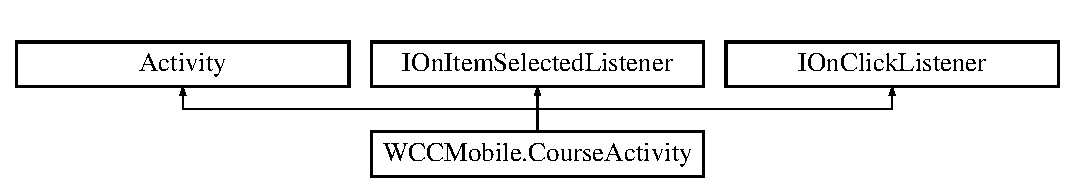
\includegraphics[height=2.000000cm]{class_w_c_c_mobile_1_1_course_activity}
\end{center}
\end{figure}
\subsection*{Public Member Functions}
\begin{DoxyCompactItemize}
\item 
void {\bfseries Open\+Courses\+File} ()\hypertarget{class_w_c_c_mobile_1_1_course_activity_add9cdaf0a170809a3b28ec893e7a6d3e}{}\label{class_w_c_c_mobile_1_1_course_activity_add9cdaf0a170809a3b28ec893e7a6d3e}

\item 
void {\bfseries Save\+Courses\+File} ()\hypertarget{class_w_c_c_mobile_1_1_course_activity_a64742fbf23cc017d0fdcc799858406ab}{}\label{class_w_c_c_mobile_1_1_course_activity_a64742fbf23cc017d0fdcc799858406ab}

\item 
void {\bfseries On\+Item\+Selected} (Adapter\+View parent, View view, int position, long id)\hypertarget{class_w_c_c_mobile_1_1_course_activity_a82383b5b14c39c8db5e35d2d77c32bcb}{}\label{class_w_c_c_mobile_1_1_course_activity_a82383b5b14c39c8db5e35d2d77c32bcb}

\item 
void {\bfseries On\+Nothing\+Selected} (Adapter\+View parent)\hypertarget{class_w_c_c_mobile_1_1_course_activity_afe39bb0b1180a44ec6f399f1b00e84a8}{}\label{class_w_c_c_mobile_1_1_course_activity_afe39bb0b1180a44ec6f399f1b00e84a8}

\item 
Boolean {\bfseries Is\+Valid\+Course} ()\hypertarget{class_w_c_c_mobile_1_1_course_activity_a8ccc690fa9d952d1866bb7ed87289793}{}\label{class_w_c_c_mobile_1_1_course_activity_a8ccc690fa9d952d1866bb7ed87289793}

\item 
void \hyperlink{class_w_c_c_mobile_1_1_course_activity_ac111acfa5c595a939bf2c7fc0ff5e0a6}{Save\+Course} ()
\begin{DoxyCompactList}\small\item\em Handles saving the current course that the manager has setup. Saves the course. \end{DoxyCompactList}\item 
void {\bfseries Open\+Course} ()\hypertarget{class_w_c_c_mobile_1_1_course_activity_af622fc93b9cd46710e3bb2f597b79da1}{}\label{class_w_c_c_mobile_1_1_course_activity_af622fc93b9cd46710e3bb2f597b79da1}

\item 
void {\bfseries Delete\+Course} ()\hypertarget{class_w_c_c_mobile_1_1_course_activity_a7549958d3c3184451bffada965cccb03}{}\label{class_w_c_c_mobile_1_1_course_activity_a7549958d3c3184451bffada965cccb03}

\item 
void {\bfseries Save\+Day} ()\hypertarget{class_w_c_c_mobile_1_1_course_activity_a7562e44ddd13638257c79cbe0e607a92}{}\label{class_w_c_c_mobile_1_1_course_activity_a7562e44ddd13638257c79cbe0e607a92}

\item 
void {\bfseries Open\+Day} ()\hypertarget{class_w_c_c_mobile_1_1_course_activity_a4e9ca8143284a6cc6d465bfcf7584ea2}{}\label{class_w_c_c_mobile_1_1_course_activity_a4e9ca8143284a6cc6d465bfcf7584ea2}

\item 
void {\bfseries open\+Day\+Alert\+Handler} (object sender, Dialog\+Click\+Event\+Args e)\hypertarget{class_w_c_c_mobile_1_1_course_activity_a3f60722ba489ba2375eab1c0dfcce310}{}\label{class_w_c_c_mobile_1_1_course_activity_a3f60722ba489ba2375eab1c0dfcce310}

\item 
void {\bfseries Delete\+Day} ()\hypertarget{class_w_c_c_mobile_1_1_course_activity_abe497f8f32f3c06c9a6ab92269033af7}{}\label{class_w_c_c_mobile_1_1_course_activity_abe497f8f32f3c06c9a6ab92269033af7}

\item 
void {\bfseries delete\+Day\+Alert\+Handler} (object sender, Dialog\+Click\+Event\+Args e)\hypertarget{class_w_c_c_mobile_1_1_course_activity_ae291e7fc41929f0a7c2c63a167b5a2ad}{}\label{class_w_c_c_mobile_1_1_course_activity_ae291e7fc41929f0a7c2c63a167b5a2ad}

\item 
void {\bfseries On\+Click} (View v)\hypertarget{class_w_c_c_mobile_1_1_course_activity_a1927be1b7a214bc605a1398d4377f460}{}\label{class_w_c_c_mobile_1_1_course_activity_a1927be1b7a214bc605a1398d4377f460}

\end{DoxyCompactItemize}
\subsection*{Protected Member Functions}
\begin{DoxyCompactItemize}
\item 
override void {\bfseries On\+Create} (Bundle saved\+Instance\+State)\hypertarget{class_w_c_c_mobile_1_1_course_activity_a5094d8dad8b79ba3e929c51773f17033}{}\label{class_w_c_c_mobile_1_1_course_activity_a5094d8dad8b79ba3e929c51773f17033}

\end{DoxyCompactItemize}
\subsection*{Properties}
\begin{DoxyCompactItemize}
\item 
static \hyperlink{class_w_c_c_mobile_1_1_course_activity}{Course\+Activity} {\bfseries singleR}\hspace{0.3cm}{\ttfamily  \mbox{[}get\mbox{]}}\hypertarget{class_w_c_c_mobile_1_1_course_activity_a2765feb543b0057f560759c06ec8b490}{}\label{class_w_c_c_mobile_1_1_course_activity_a2765feb543b0057f560759c06ec8b490}

\item 
Toast {\bfseries T\+O\+A\+ST}\hspace{0.3cm}{\ttfamily  \mbox{[}get\mbox{]}}\hypertarget{class_w_c_c_mobile_1_1_course_activity_a12c725317d66167d9e1c9c78b7ee70cf}{}\label{class_w_c_c_mobile_1_1_course_activity_a12c725317d66167d9e1c9c78b7ee70cf}

\end{DoxyCompactItemize}


\subsection{Member Function Documentation}
\index{W\+C\+C\+Mobile\+::\+Course\+Activity@{W\+C\+C\+Mobile\+::\+Course\+Activity}!Save\+Course@{Save\+Course}}
\index{Save\+Course@{Save\+Course}!W\+C\+C\+Mobile\+::\+Course\+Activity@{W\+C\+C\+Mobile\+::\+Course\+Activity}}
\subsubsection[{\texorpdfstring{Save\+Course()}{SaveCourse()}}]{\setlength{\rightskip}{0pt plus 5cm}void W\+C\+C\+Mobile.\+Course\+Activity.\+Save\+Course (
\begin{DoxyParamCaption}
{}
\end{DoxyParamCaption}
)}\hypertarget{class_w_c_c_mobile_1_1_course_activity_ac111acfa5c595a939bf2c7fc0ff5e0a6}{}\label{class_w_c_c_mobile_1_1_course_activity_ac111acfa5c595a939bf2c7fc0ff5e0a6}


Handles saving the current course that the manager has setup. Saves the course. 



The documentation for this class was generated from the following file\+:\begin{DoxyCompactItemize}
\item 
Source/\+Activities/Course\+Activity.\+cs\end{DoxyCompactItemize}

\hypertarget{class_w_c_c_mobile_1_1_course_1_1_course_day}{}\section{W\+C\+C\+Mobile.\+Course.\+Course\+Day Class Reference}
\label{class_w_c_c_mobile_1_1_course_1_1_course_day}\index{W\+C\+C\+Mobile.\+Course.\+Course\+Day@{W\+C\+C\+Mobile.\+Course.\+Course\+Day}}
\subsection*{Public Member Functions}
\begin{DoxyCompactItemize}
\item 
{\bfseries Course\+Day} (string day, string start\+Time\+Stamp, string start\+Mer, string end\+Time\+Stamp, string end\+Mer)\hypertarget{class_w_c_c_mobile_1_1_course_1_1_course_day_a67d05ee4d3adf8109f948a421618786c}{}\label{class_w_c_c_mobile_1_1_course_1_1_course_day_a67d05ee4d3adf8109f948a421618786c}

\item 
void {\bfseries Update} (string day, string start\+Time\+Stamp, string start\+Mer, string end\+Time\+Stamp, string end\+Mer)\hypertarget{class_w_c_c_mobile_1_1_course_1_1_course_day_afc1f017708bc8412fe886f9902339a14}{}\label{class_w_c_c_mobile_1_1_course_1_1_course_day_afc1f017708bc8412fe886f9902339a14}

\end{DoxyCompactItemize}
\subsection*{Properties}
\begin{DoxyCompactItemize}
\item 
string {\bfseries D\+AY}\hspace{0.3cm}{\ttfamily  \mbox{[}get\mbox{]}}\hypertarget{class_w_c_c_mobile_1_1_course_1_1_course_day_a1174d20f23091bde693b7990d26245f4}{}\label{class_w_c_c_mobile_1_1_course_1_1_course_day_a1174d20f23091bde693b7990d26245f4}

\item 
Time\+Span {\bfseries S\+T\+A\+R\+T\+\_\+\+T\+I\+ME}\hspace{0.3cm}{\ttfamily  \mbox{[}get\mbox{]}}\hypertarget{class_w_c_c_mobile_1_1_course_1_1_course_day_a60c185be582a6b10ad5c15045d3fdb1f}{}\label{class_w_c_c_mobile_1_1_course_1_1_course_day_a60c185be582a6b10ad5c15045d3fdb1f}

\item 
Time\+Span {\bfseries E\+N\+D\+\_\+\+T\+I\+ME}\hspace{0.3cm}{\ttfamily  \mbox{[}get\mbox{]}}\hypertarget{class_w_c_c_mobile_1_1_course_1_1_course_day_a549d55a789ac8a7b0fa26f7ba6df4718}{}\label{class_w_c_c_mobile_1_1_course_1_1_course_day_a549d55a789ac8a7b0fa26f7ba6df4718}

\end{DoxyCompactItemize}


The documentation for this class was generated from the following file\+:\begin{DoxyCompactItemize}
\item 
Source/\+Activities/Course\+Activity.\+cs\end{DoxyCompactItemize}

\hypertarget{class_w_c_c_mobile_1_1_disk_cache}{}\section{W\+C\+C\+Mobile.\+Disk\+Cache Class Reference}
\label{class_w_c_c_mobile_1_1_disk_cache}\index{W\+C\+C\+Mobile.\+Disk\+Cache@{W\+C\+C\+Mobile.\+Disk\+Cache}}
\subsection*{Public Member Functions}
\begin{DoxyCompactItemize}
\item 
{\bfseries Disk\+Cache} (string base\+Path, string version)\hypertarget{class_w_c_c_mobile_1_1_disk_cache_a40a1b6ff0702cfb23d2185c51e69af35}{}\label{class_w_c_c_mobile_1_1_disk_cache_a40a1b6ff0702cfb23d2185c51e69af35}

\item 
void {\bfseries Add\+Or\+Update} (string key, Bitmap bmp, Time\+Span duration)\hypertarget{class_w_c_c_mobile_1_1_disk_cache_a92e72251d1a9ed2dac403931606da23b}{}\label{class_w_c_c_mobile_1_1_disk_cache_a92e72251d1a9ed2dac403931606da23b}

\item 
bool {\bfseries Try\+Get} (string key, out Bitmap bmp)\hypertarget{class_w_c_c_mobile_1_1_disk_cache_a994805d57caa75e7b2b7056e61c85cbd}{}\label{class_w_c_c_mobile_1_1_disk_cache_a994805d57caa75e7b2b7056e61c85cbd}

\end{DoxyCompactItemize}
\subsection*{Static Public Member Functions}
\begin{DoxyCompactItemize}
\item 
static \hyperlink{class_w_c_c_mobile_1_1_disk_cache}{Disk\+Cache} {\bfseries Create\+Cache} (Android.\+Content.\+Context ctx, string cache\+Name, string version=\char`\"{}1.\+0\char`\"{})\hypertarget{class_w_c_c_mobile_1_1_disk_cache_a8fdcd5e0485803abcd5bffc663cc03ef}{}\label{class_w_c_c_mobile_1_1_disk_cache_a8fdcd5e0485803abcd5bffc663cc03ef}

\end{DoxyCompactItemize}


The documentation for this class was generated from the following file\+:\begin{DoxyCompactItemize}
\item 
Source/\+Storage/Disk\+Cache.\+cs\end{DoxyCompactItemize}

\hypertarget{class_w_c_c_mobile_1_1_drawer_around_adapter}{}\section{W\+C\+C\+Mobile.\+Drawer\+Around\+Adapter Class Reference}
\label{class_w_c_c_mobile_1_1_drawer_around_adapter}\index{W\+C\+C\+Mobile.\+Drawer\+Around\+Adapter@{W\+C\+C\+Mobile.\+Drawer\+Around\+Adapter}}
Inheritance diagram for W\+C\+C\+Mobile.\+Drawer\+Around\+Adapter\+:\begin{figure}[H]
\begin{center}
\leavevmode
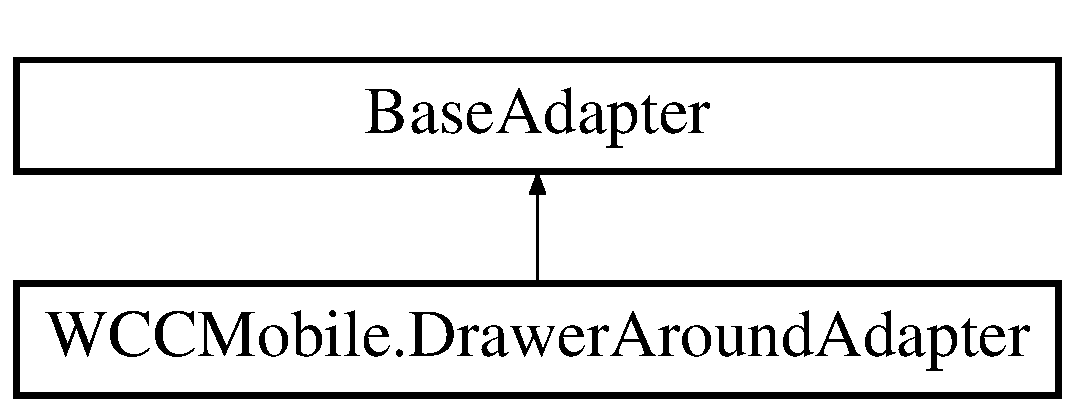
\includegraphics[height=2.000000cm]{class_w_c_c_mobile_1_1_drawer_around_adapter}
\end{center}
\end{figure}
\subsection*{Public Member Functions}
\begin{DoxyCompactItemize}
\item 
{\bfseries Drawer\+Around\+Adapter} (Context context)\hypertarget{class_w_c_c_mobile_1_1_drawer_around_adapter_aab98fef8ac6bf8ba811cee127284b60a}{}\label{class_w_c_c_mobile_1_1_drawer_around_adapter_aab98fef8ac6bf8ba811cee127284b60a}

\item 
void {\bfseries Set\+Schedule} (\hyperlink{class_w_c_c_mobile_1_1_models_1_1_schedule_item}{Schedule\+Item}\mbox{[}$\,$\mbox{]} schedule)\hypertarget{class_w_c_c_mobile_1_1_drawer_around_adapter_aa54a7dbf8ed5a7765a5e423d6389d23b}{}\label{class_w_c_c_mobile_1_1_drawer_around_adapter_aa54a7dbf8ed5a7765a5e423d6389d23b}

\item 
void {\bfseries Refresh} ()\hypertarget{class_w_c_c_mobile_1_1_drawer_around_adapter_a79a2da6a7abad5f86e077d3b51a6555d}{}\label{class_w_c_c_mobile_1_1_drawer_around_adapter_a79a2da6a7abad5f86e077d3b51a6555d}

\item 
override Java.\+Lang.\+Object {\bfseries Get\+Item} (int position)\hypertarget{class_w_c_c_mobile_1_1_drawer_around_adapter_a38aa96cdccda8d2573eca6bd00eb1a77}{}\label{class_w_c_c_mobile_1_1_drawer_around_adapter_a38aa96cdccda8d2573eca6bd00eb1a77}

\item 
override long {\bfseries Get\+Item\+Id} (int position)\hypertarget{class_w_c_c_mobile_1_1_drawer_around_adapter_a7218feb737992d13d7ea203487a4136f}{}\label{class_w_c_c_mobile_1_1_drawer_around_adapter_a7218feb737992d13d7ea203487a4136f}

\item 
override View {\bfseries Get\+View} (int position, View convert\+View, View\+Group parent)\hypertarget{class_w_c_c_mobile_1_1_drawer_around_adapter_a0e69bb0ee5bc2234514cf4668c67b79a}{}\label{class_w_c_c_mobile_1_1_drawer_around_adapter_a0e69bb0ee5bc2234514cf4668c67b79a}

\item 
override bool {\bfseries Is\+Enabled} (int position)\hypertarget{class_w_c_c_mobile_1_1_drawer_around_adapter_a78b1ed19fd3e9b7e48d9e56a06071867}{}\label{class_w_c_c_mobile_1_1_drawer_around_adapter_a78b1ed19fd3e9b7e48d9e56a06071867}

\item 
override bool {\bfseries Are\+All\+Items\+Enabled} ()\hypertarget{class_w_c_c_mobile_1_1_drawer_around_adapter_a6603b435c5a8c334bd0280bc29ce2893}{}\label{class_w_c_c_mobile_1_1_drawer_around_adapter_a6603b435c5a8c334bd0280bc29ce2893}

\end{DoxyCompactItemize}
\subsection*{Properties}
\begin{DoxyCompactItemize}
\item 
override int {\bfseries Count}\hspace{0.3cm}{\ttfamily  \mbox{[}get\mbox{]}}\hypertarget{class_w_c_c_mobile_1_1_drawer_around_adapter_a1e79a8c77850ad4572f772e01b6d1fe9}{}\label{class_w_c_c_mobile_1_1_drawer_around_adapter_a1e79a8c77850ad4572f772e01b6d1fe9}

\end{DoxyCompactItemize}


The documentation for this class was generated from the following file\+:\begin{DoxyCompactItemize}
\item 
Source/\+Activities/Campus\+Map\+Activity.\+cs\end{DoxyCompactItemize}

\hypertarget{class_w_c_c_mobile_1_1_drawer_menu_adapter}{}\section{W\+C\+C\+Mobile.\+Drawer\+Menu\+Adapter Class Reference}
\label{class_w_c_c_mobile_1_1_drawer_menu_adapter}\index{W\+C\+C\+Mobile.\+Drawer\+Menu\+Adapter@{W\+C\+C\+Mobile.\+Drawer\+Menu\+Adapter}}
Inheritance diagram for W\+C\+C\+Mobile.\+Drawer\+Menu\+Adapter\+:\begin{figure}[H]
\begin{center}
\leavevmode
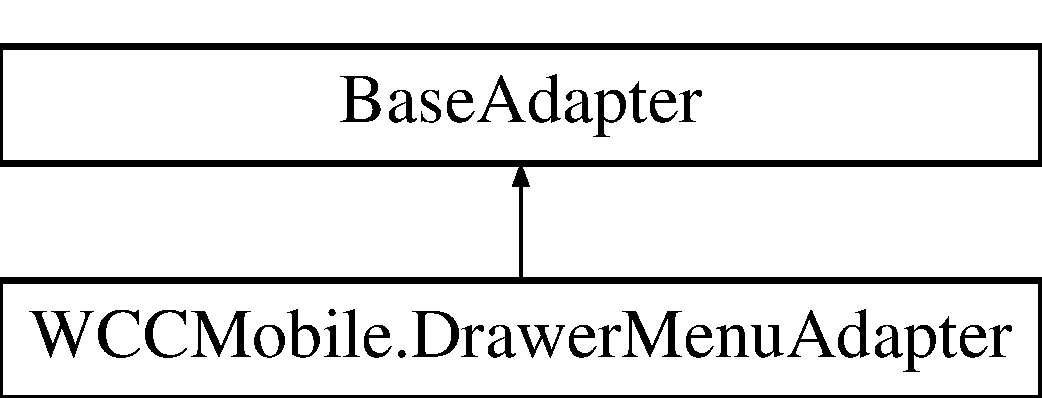
\includegraphics[height=2.000000cm]{class_w_c_c_mobile_1_1_drawer_menu_adapter}
\end{center}
\end{figure}
\subsection*{Public Member Functions}
\begin{DoxyCompactItemize}
\item 
{\bfseries Drawer\+Menu\+Adapter} (Context context)\hypertarget{class_w_c_c_mobile_1_1_drawer_menu_adapter_ae1a0b37a2a1a30f8a0bb4c69893803cd}{}\label{class_w_c_c_mobile_1_1_drawer_menu_adapter_ae1a0b37a2a1a30f8a0bb4c69893803cd}

\item 
override Java.\+Lang.\+Object {\bfseries Get\+Item} (int position)\hypertarget{class_w_c_c_mobile_1_1_drawer_menu_adapter_afc38d1f1905b7ff184992c99602aff12}{}\label{class_w_c_c_mobile_1_1_drawer_menu_adapter_afc38d1f1905b7ff184992c99602aff12}

\item 
override long {\bfseries Get\+Item\+Id} (int position)\hypertarget{class_w_c_c_mobile_1_1_drawer_menu_adapter_a86d770733c700b289e44d6b6838ed2c2}{}\label{class_w_c_c_mobile_1_1_drawer_menu_adapter_a86d770733c700b289e44d6b6838ed2c2}

\item 
override View {\bfseries Get\+View} (int position, View convert\+View, View\+Group parent)\hypertarget{class_w_c_c_mobile_1_1_drawer_menu_adapter_a9ff22a632e5ecdff86a9e0e23dbf234d}{}\label{class_w_c_c_mobile_1_1_drawer_menu_adapter_a9ff22a632e5ecdff86a9e0e23dbf234d}

\item 
override bool {\bfseries Is\+Enabled} (int position)\hypertarget{class_w_c_c_mobile_1_1_drawer_menu_adapter_abdeac51f7a3e4461e4c2db93aed049e3}{}\label{class_w_c_c_mobile_1_1_drawer_menu_adapter_abdeac51f7a3e4461e4c2db93aed049e3}

\item 
override bool {\bfseries Are\+All\+Items\+Enabled} ()\hypertarget{class_w_c_c_mobile_1_1_drawer_menu_adapter_a74706ad66ad2ca6100ad0d2b9bf19b0d}{}\label{class_w_c_c_mobile_1_1_drawer_menu_adapter_a74706ad66ad2ca6100ad0d2b9bf19b0d}

\end{DoxyCompactItemize}
\subsection*{Properties}
\begin{DoxyCompactItemize}
\item 
override int {\bfseries Count}\hspace{0.3cm}{\ttfamily  \mbox{[}get\mbox{]}}\hypertarget{class_w_c_c_mobile_1_1_drawer_menu_adapter_afe4d6b612f857db6cfa993d46c7bd449}{}\label{class_w_c_c_mobile_1_1_drawer_menu_adapter_afe4d6b612f857db6cfa993d46c7bd449}

\end{DoxyCompactItemize}


The documentation for this class was generated from the following file\+:\begin{DoxyCompactItemize}
\item 
Source/\+Activities/Campus\+Map\+Activity.\+cs\end{DoxyCompactItemize}

\hypertarget{class_w_c_c_mobile_1_1_error_dialog_fragment}{}\section{W\+C\+C\+Mobile.\+Error\+Dialog\+Fragment Class Reference}
\label{class_w_c_c_mobile_1_1_error_dialog_fragment}\index{W\+C\+C\+Mobile.\+Error\+Dialog\+Fragment@{W\+C\+C\+Mobile.\+Error\+Dialog\+Fragment}}
Inheritance diagram for W\+C\+C\+Mobile.\+Error\+Dialog\+Fragment\+:\begin{figure}[H]
\begin{center}
\leavevmode
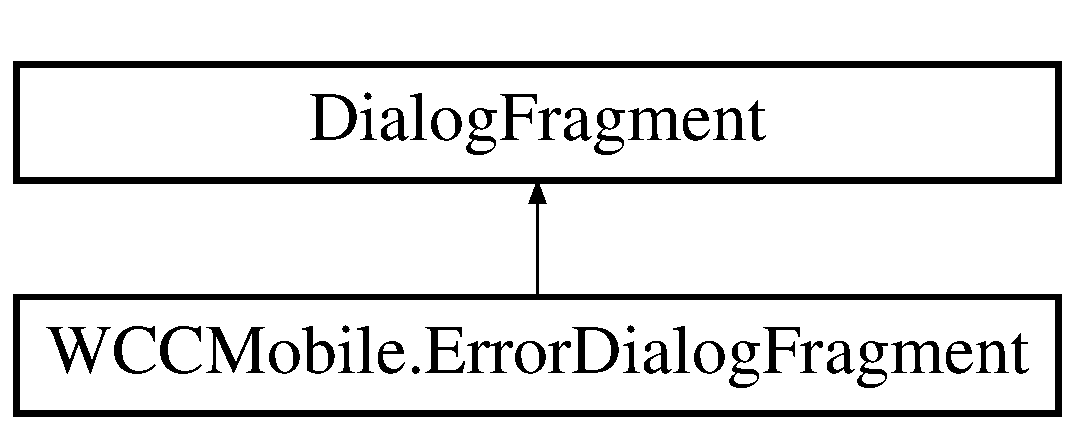
\includegraphics[height=2.000000cm]{class_w_c_c_mobile_1_1_error_dialog_fragment}
\end{center}
\end{figure}
\subsection*{Public Member Functions}
\begin{DoxyCompactItemize}
\item 
override Dialog \hyperlink{class_w_c_c_mobile_1_1_error_dialog_fragment_a50bd333dad2d7cb06d5749bb556681fd}{On\+Create\+Dialog} (Bundle saved\+Instance\+State)
\begin{DoxyCompactList}\small\item\em Called when \mbox{[}create dialog\mbox{]}. \end{DoxyCompactList}\end{DoxyCompactItemize}
\subsection*{Properties}
\begin{DoxyCompactItemize}
\item 
new Dialog {\bfseries Dialog}\hspace{0.3cm}{\ttfamily  \mbox{[}get, set\mbox{]}}\hypertarget{class_w_c_c_mobile_1_1_error_dialog_fragment_a611f4dc57228edabc30f3f87eef38608}{}\label{class_w_c_c_mobile_1_1_error_dialog_fragment_a611f4dc57228edabc30f3f87eef38608}

\end{DoxyCompactItemize}


\subsection{Member Function Documentation}
\index{W\+C\+C\+Mobile\+::\+Error\+Dialog\+Fragment@{W\+C\+C\+Mobile\+::\+Error\+Dialog\+Fragment}!On\+Create\+Dialog@{On\+Create\+Dialog}}
\index{On\+Create\+Dialog@{On\+Create\+Dialog}!W\+C\+C\+Mobile\+::\+Error\+Dialog\+Fragment@{W\+C\+C\+Mobile\+::\+Error\+Dialog\+Fragment}}
\subsubsection[{\texorpdfstring{On\+Create\+Dialog(\+Bundle saved\+Instance\+State)}{OnCreateDialog(Bundle savedInstanceState)}}]{\setlength{\rightskip}{0pt plus 5cm}override Dialog W\+C\+C\+Mobile.\+Error\+Dialog\+Fragment.\+On\+Create\+Dialog (
\begin{DoxyParamCaption}
\item[{Bundle}]{saved\+Instance\+State}
\end{DoxyParamCaption}
)}\hypertarget{class_w_c_c_mobile_1_1_error_dialog_fragment_a50bd333dad2d7cb06d5749bb556681fd}{}\label{class_w_c_c_mobile_1_1_error_dialog_fragment_a50bd333dad2d7cb06d5749bb556681fd}


Called when \mbox{[}create dialog\mbox{]}. 


\begin{DoxyParams}{Parameters}
{\em saved\+Instance\+State} & State of the saved instance.\\
\hline
\end{DoxyParams}
\begin{DoxyReturn}{Returns}

\end{DoxyReturn}


The documentation for this class was generated from the following file\+:\begin{DoxyCompactItemize}
\item 
Source/\+Activities/Campus\+Map\+Activity.\+cs\end{DoxyCompactItemize}

\hypertarget{class_w_c_c_mobile_1_1_adapters_1_1_generic_adapter}{}\section{W\+C\+C\+Mobile.\+Adapters.\+Generic\+Adapter$<$ T, X $>$ Class Template Reference}
\label{class_w_c_c_mobile_1_1_adapters_1_1_generic_adapter}\index{W\+C\+C\+Mobile.\+Adapters.\+Generic\+Adapter$<$ T, X $>$@{W\+C\+C\+Mobile.\+Adapters.\+Generic\+Adapter$<$ T, X $>$}}
Inheritance diagram for W\+C\+C\+Mobile.\+Adapters.\+Generic\+Adapter$<$ T, X $>$\+:\begin{figure}[H]
\begin{center}
\leavevmode
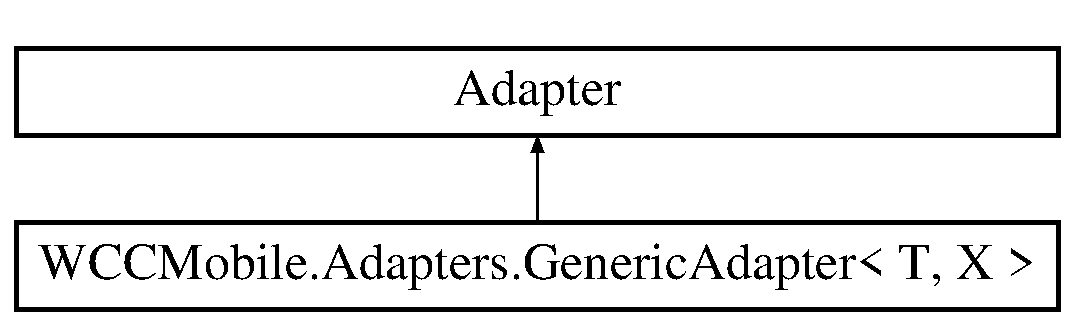
\includegraphics[height=2.000000cm]{class_w_c_c_mobile_1_1_adapters_1_1_generic_adapter}
\end{center}
\end{figure}
\subsection*{Public Member Functions}
\begin{DoxyCompactItemize}
\item 
\hyperlink{class_w_c_c_mobile_1_1_adapters_1_1_generic_adapter_af243e0f38786848e559ccaec47243455}{Generic\+Adapter} (I\+List$<$ T $>$ \hyperlink{class_w_c_c_mobile_1_1_adapters_1_1_generic_adapter_a7d82f417d14c6d0027dfb56cd3361c76}{items}, int \hyperlink{class_w_c_c_mobile_1_1_adapters_1_1_generic_adapter_a2adf5c93b6f5abaf8c51e28a9a91c6d3}{resource\+Id}, Func$<$ View, X $>$ \hyperlink{class_w_c_c_mobile_1_1_adapters_1_1_generic_adapter_ad2341fe4f922682e52dc4d86f397868f}{creator})
\begin{DoxyCompactList}\small\item\em Initializes a new instance of the \hyperlink{class_w_c_c_mobile_1_1_adapters_1_1_generic_adapter_af243e0f38786848e559ccaec47243455}{Generic\+Adapter$<$\+T, X$>$} class. \end{DoxyCompactList}\item 
void \hyperlink{class_w_c_c_mobile_1_1_adapters_1_1_generic_adapter_a2737389fa7ce0bf841be29b36aaedd0c}{Set\+List\+Items} (I\+List$<$ T $>$ \hyperlink{class_w_c_c_mobile_1_1_adapters_1_1_generic_adapter_a7d82f417d14c6d0027dfb56cd3361c76}{items})
\begin{DoxyCompactList}\small\item\em Sets the list items. \end{DoxyCompactList}\item 
override void \hyperlink{class_w_c_c_mobile_1_1_adapters_1_1_generic_adapter_a3f0945aae956db3dc6a50c954d93dfd5}{On\+Bind\+View\+Holder} (Recycler\+View.\+View\+Holder holder, int position)
\begin{DoxyCompactList}\small\item\em Called when \mbox{[}bind view holder\mbox{]}. \end{DoxyCompactList}\item 
override Recycler\+View.\+View\+Holder \hyperlink{class_w_c_c_mobile_1_1_adapters_1_1_generic_adapter_a363c83b72c77420b2ec8df91cd98b4fa}{On\+Create\+View\+Holder} (Android.\+Views.\+View\+Group parent, int view\+Type)
\begin{DoxyCompactList}\small\item\em Called when \mbox{[}create view holder\mbox{]}. \end{DoxyCompactList}\end{DoxyCompactItemize}
\subsection*{Properties}
\begin{DoxyCompactItemize}
\item 
I\+List$<$ T $>$ \hyperlink{class_w_c_c_mobile_1_1_adapters_1_1_generic_adapter_a7d82f417d14c6d0027dfb56cd3361c76}{items}\hspace{0.3cm}{\ttfamily  \mbox{[}get\mbox{]}}
\begin{DoxyCompactList}\small\item\em Gets the items. \end{DoxyCompactList}\item 
int \hyperlink{class_w_c_c_mobile_1_1_adapters_1_1_generic_adapter_a2adf5c93b6f5abaf8c51e28a9a91c6d3}{resource\+Id}\hspace{0.3cm}{\ttfamily  \mbox{[}get\mbox{]}}
\begin{DoxyCompactList}\small\item\em Gets the resource identifier. \end{DoxyCompactList}\item 
Func$<$ View, X $>$ \hyperlink{class_w_c_c_mobile_1_1_adapters_1_1_generic_adapter_ad2341fe4f922682e52dc4d86f397868f}{creator}\hspace{0.3cm}{\ttfamily  \mbox{[}get\mbox{]}}
\begin{DoxyCompactList}\small\item\em Gets the creator. \end{DoxyCompactList}\item 
override int \hyperlink{class_w_c_c_mobile_1_1_adapters_1_1_generic_adapter_a6d805fdca94bdf6d91bd4cad6998cb32}{Item\+Count}\hspace{0.3cm}{\ttfamily  \mbox{[}get\mbox{]}}
\begin{DoxyCompactList}\small\item\em Gets the item count. \end{DoxyCompactList}\end{DoxyCompactItemize}
\subsection*{Events}
\begin{DoxyCompactItemize}
\item 
Event\+Handler$<$ int $>$ {\bfseries Item\+Click}\hypertarget{class_w_c_c_mobile_1_1_adapters_1_1_generic_adapter_a9f45547a182d73bc6ea90949c8fb40a1}{}\label{class_w_c_c_mobile_1_1_adapters_1_1_generic_adapter_a9f45547a182d73bc6ea90949c8fb40a1}

\end{DoxyCompactItemize}


\subsection{Constructor \& Destructor Documentation}
\index{W\+C\+C\+Mobile\+::\+Adapters\+::\+Generic\+Adapter@{W\+C\+C\+Mobile\+::\+Adapters\+::\+Generic\+Adapter}!Generic\+Adapter@{Generic\+Adapter}}
\index{Generic\+Adapter@{Generic\+Adapter}!W\+C\+C\+Mobile\+::\+Adapters\+::\+Generic\+Adapter@{W\+C\+C\+Mobile\+::\+Adapters\+::\+Generic\+Adapter}}
\subsubsection[{\texorpdfstring{Generic\+Adapter(\+I\+List$<$ T $>$ items, int resource\+Id, Func$<$ View, X $>$ creator)}{GenericAdapter(IList< T > items, int resourceId, Func< View, X > creator)}}]{\setlength{\rightskip}{0pt plus 5cm}{\bf W\+C\+C\+Mobile.\+Adapters.\+Generic\+Adapter}$<$ T, X $>$.{\bf Generic\+Adapter} (
\begin{DoxyParamCaption}
\item[{I\+List$<$ T $>$}]{items, }
\item[{int}]{resource\+Id, }
\item[{Func$<$ View, X $>$}]{creator}
\end{DoxyParamCaption}
)}\hypertarget{class_w_c_c_mobile_1_1_adapters_1_1_generic_adapter_af243e0f38786848e559ccaec47243455}{}\label{class_w_c_c_mobile_1_1_adapters_1_1_generic_adapter_af243e0f38786848e559ccaec47243455}


Initializes a new instance of the \hyperlink{class_w_c_c_mobile_1_1_adapters_1_1_generic_adapter_af243e0f38786848e559ccaec47243455}{Generic\+Adapter$<$\+T, X$>$} class. 


\begin{DoxyParams}{Parameters}
{\em items} & The items.\\
\hline
{\em resource\+Id} & The resource identifier.\\
\hline
{\em creator} & The creator.\\
\hline
\end{DoxyParams}


\subsection{Member Function Documentation}
\index{W\+C\+C\+Mobile\+::\+Adapters\+::\+Generic\+Adapter@{W\+C\+C\+Mobile\+::\+Adapters\+::\+Generic\+Adapter}!On\+Bind\+View\+Holder@{On\+Bind\+View\+Holder}}
\index{On\+Bind\+View\+Holder@{On\+Bind\+View\+Holder}!W\+C\+C\+Mobile\+::\+Adapters\+::\+Generic\+Adapter@{W\+C\+C\+Mobile\+::\+Adapters\+::\+Generic\+Adapter}}
\subsubsection[{\texorpdfstring{On\+Bind\+View\+Holder(\+Recycler\+View.\+View\+Holder holder, int position)}{OnBindViewHolder(RecyclerView.ViewHolder holder, int position)}}]{\setlength{\rightskip}{0pt plus 5cm}override void {\bf W\+C\+C\+Mobile.\+Adapters.\+Generic\+Adapter}$<$ T, X $>$.On\+Bind\+View\+Holder (
\begin{DoxyParamCaption}
\item[{Recycler\+View.\+View\+Holder}]{holder, }
\item[{int}]{position}
\end{DoxyParamCaption}
)}\hypertarget{class_w_c_c_mobile_1_1_adapters_1_1_generic_adapter_a3f0945aae956db3dc6a50c954d93dfd5}{}\label{class_w_c_c_mobile_1_1_adapters_1_1_generic_adapter_a3f0945aae956db3dc6a50c954d93dfd5}


Called when \mbox{[}bind view holder\mbox{]}. 


\begin{DoxyParams}{Parameters}
{\em holder} & The holder.\\
\hline
{\em position} & The position.\\
\hline
\end{DoxyParams}
\index{W\+C\+C\+Mobile\+::\+Adapters\+::\+Generic\+Adapter@{W\+C\+C\+Mobile\+::\+Adapters\+::\+Generic\+Adapter}!On\+Create\+View\+Holder@{On\+Create\+View\+Holder}}
\index{On\+Create\+View\+Holder@{On\+Create\+View\+Holder}!W\+C\+C\+Mobile\+::\+Adapters\+::\+Generic\+Adapter@{W\+C\+C\+Mobile\+::\+Adapters\+::\+Generic\+Adapter}}
\subsubsection[{\texorpdfstring{On\+Create\+View\+Holder(\+Android.\+Views.\+View\+Group parent, int view\+Type)}{OnCreateViewHolder(Android.Views.ViewGroup parent, int viewType)}}]{\setlength{\rightskip}{0pt plus 5cm}override Recycler\+View.\+View\+Holder {\bf W\+C\+C\+Mobile.\+Adapters.\+Generic\+Adapter}$<$ T, X $>$.On\+Create\+View\+Holder (
\begin{DoxyParamCaption}
\item[{Android.\+Views.\+View\+Group}]{parent, }
\item[{int}]{view\+Type}
\end{DoxyParamCaption}
)}\hypertarget{class_w_c_c_mobile_1_1_adapters_1_1_generic_adapter_a363c83b72c77420b2ec8df91cd98b4fa}{}\label{class_w_c_c_mobile_1_1_adapters_1_1_generic_adapter_a363c83b72c77420b2ec8df91cd98b4fa}


Called when \mbox{[}create view holder\mbox{]}. 


\begin{DoxyParams}{Parameters}
{\em parent} & The parent.\\
\hline
{\em view\+Type} & Type of the view.\\
\hline
\end{DoxyParams}
\begin{DoxyReturn}{Returns}

\end{DoxyReturn}
\index{W\+C\+C\+Mobile\+::\+Adapters\+::\+Generic\+Adapter@{W\+C\+C\+Mobile\+::\+Adapters\+::\+Generic\+Adapter}!Set\+List\+Items@{Set\+List\+Items}}
\index{Set\+List\+Items@{Set\+List\+Items}!W\+C\+C\+Mobile\+::\+Adapters\+::\+Generic\+Adapter@{W\+C\+C\+Mobile\+::\+Adapters\+::\+Generic\+Adapter}}
\subsubsection[{\texorpdfstring{Set\+List\+Items(\+I\+List$<$ T $>$ items)}{SetListItems(IList< T > items)}}]{\setlength{\rightskip}{0pt plus 5cm}void {\bf W\+C\+C\+Mobile.\+Adapters.\+Generic\+Adapter}$<$ T, X $>$.Set\+List\+Items (
\begin{DoxyParamCaption}
\item[{I\+List$<$ T $>$}]{items}
\end{DoxyParamCaption}
)}\hypertarget{class_w_c_c_mobile_1_1_adapters_1_1_generic_adapter_a2737389fa7ce0bf841be29b36aaedd0c}{}\label{class_w_c_c_mobile_1_1_adapters_1_1_generic_adapter_a2737389fa7ce0bf841be29b36aaedd0c}


Sets the list items. 


\begin{DoxyParams}{Parameters}
{\em items} & The items.\\
\hline
\end{DoxyParams}


\subsection{Property Documentation}
\index{W\+C\+C\+Mobile\+::\+Adapters\+::\+Generic\+Adapter@{W\+C\+C\+Mobile\+::\+Adapters\+::\+Generic\+Adapter}!creator@{creator}}
\index{creator@{creator}!W\+C\+C\+Mobile\+::\+Adapters\+::\+Generic\+Adapter@{W\+C\+C\+Mobile\+::\+Adapters\+::\+Generic\+Adapter}}
\subsubsection[{\texorpdfstring{creator}{creator}}]{\setlength{\rightskip}{0pt plus 5cm}Func$<$View, X$>$ {\bf W\+C\+C\+Mobile.\+Adapters.\+Generic\+Adapter}$<$ T, X $>$.creator\hspace{0.3cm}{\ttfamily [get]}}\hypertarget{class_w_c_c_mobile_1_1_adapters_1_1_generic_adapter_ad2341fe4f922682e52dc4d86f397868f}{}\label{class_w_c_c_mobile_1_1_adapters_1_1_generic_adapter_ad2341fe4f922682e52dc4d86f397868f}


Gets the creator. 

The creator. \index{W\+C\+C\+Mobile\+::\+Adapters\+::\+Generic\+Adapter@{W\+C\+C\+Mobile\+::\+Adapters\+::\+Generic\+Adapter}!Item\+Count@{Item\+Count}}
\index{Item\+Count@{Item\+Count}!W\+C\+C\+Mobile\+::\+Adapters\+::\+Generic\+Adapter@{W\+C\+C\+Mobile\+::\+Adapters\+::\+Generic\+Adapter}}
\subsubsection[{\texorpdfstring{Item\+Count}{ItemCount}}]{\setlength{\rightskip}{0pt plus 5cm}override int {\bf W\+C\+C\+Mobile.\+Adapters.\+Generic\+Adapter}$<$ T, X $>$.Item\+Count\hspace{0.3cm}{\ttfamily [get]}}\hypertarget{class_w_c_c_mobile_1_1_adapters_1_1_generic_adapter_a6d805fdca94bdf6d91bd4cad6998cb32}{}\label{class_w_c_c_mobile_1_1_adapters_1_1_generic_adapter_a6d805fdca94bdf6d91bd4cad6998cb32}


Gets the item count. 

The item count. \index{W\+C\+C\+Mobile\+::\+Adapters\+::\+Generic\+Adapter@{W\+C\+C\+Mobile\+::\+Adapters\+::\+Generic\+Adapter}!items@{items}}
\index{items@{items}!W\+C\+C\+Mobile\+::\+Adapters\+::\+Generic\+Adapter@{W\+C\+C\+Mobile\+::\+Adapters\+::\+Generic\+Adapter}}
\subsubsection[{\texorpdfstring{items}{items}}]{\setlength{\rightskip}{0pt plus 5cm}I\+List$<$T$>$ {\bf W\+C\+C\+Mobile.\+Adapters.\+Generic\+Adapter}$<$ T, X $>$.items\hspace{0.3cm}{\ttfamily [get]}}\hypertarget{class_w_c_c_mobile_1_1_adapters_1_1_generic_adapter_a7d82f417d14c6d0027dfb56cd3361c76}{}\label{class_w_c_c_mobile_1_1_adapters_1_1_generic_adapter_a7d82f417d14c6d0027dfb56cd3361c76}


Gets the items. 

The items. \index{W\+C\+C\+Mobile\+::\+Adapters\+::\+Generic\+Adapter@{W\+C\+C\+Mobile\+::\+Adapters\+::\+Generic\+Adapter}!resource\+Id@{resource\+Id}}
\index{resource\+Id@{resource\+Id}!W\+C\+C\+Mobile\+::\+Adapters\+::\+Generic\+Adapter@{W\+C\+C\+Mobile\+::\+Adapters\+::\+Generic\+Adapter}}
\subsubsection[{\texorpdfstring{resource\+Id}{resourceId}}]{\setlength{\rightskip}{0pt plus 5cm}int {\bf W\+C\+C\+Mobile.\+Adapters.\+Generic\+Adapter}$<$ T, X $>$.resource\+Id\hspace{0.3cm}{\ttfamily [get]}}\hypertarget{class_w_c_c_mobile_1_1_adapters_1_1_generic_adapter_a2adf5c93b6f5abaf8c51e28a9a91c6d3}{}\label{class_w_c_c_mobile_1_1_adapters_1_1_generic_adapter_a2adf5c93b6f5abaf8c51e28a9a91c6d3}


Gets the resource identifier. 

The resource identifier. 

The documentation for this class was generated from the following file\+:\begin{DoxyCompactItemize}
\item 
Source/\+Adapters/Generic\+Adapter.\+cs\end{DoxyCompactItemize}

\hypertarget{class_w_c_c_mobile_1_1_get_map_helper}{}\section{W\+C\+C\+Mobile.\+Get\+Map\+Helper Class Reference}
\label{class_w_c_c_mobile_1_1_get_map_helper}\index{W\+C\+C\+Mobile.\+Get\+Map\+Helper@{W\+C\+C\+Mobile.\+Get\+Map\+Helper}}


This class is not currently to be used. It should be removed as we are using Map\+View as the map control not Map\+Fragment.  


Inheritance diagram for W\+C\+C\+Mobile.\+Get\+Map\+Helper\+:\begin{figure}[H]
\begin{center}
\leavevmode
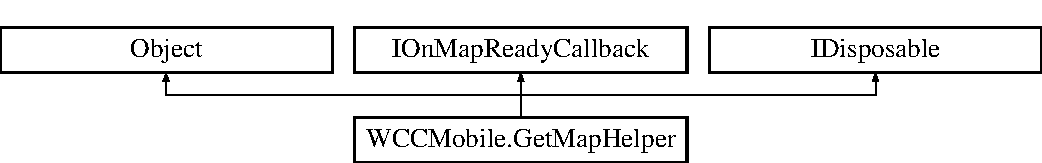
\includegraphics[height=2.000000cm]{class_w_c_c_mobile_1_1_get_map_helper}
\end{center}
\end{figure}
\subsection*{Public Member Functions}
\begin{DoxyCompactItemize}
\item 
\hyperlink{class_w_c_c_mobile_1_1_get_map_helper_a505dc62eaa5505585193f426c02c3d21}{Get\+Map\+Helper} ()
\begin{DoxyCompactList}\small\item\em Initializes a new instance of the \hyperlink{class_w_c_c_mobile_1_1_get_map_helper}{Get\+Map\+Helper} class. \end{DoxyCompactList}\item 
async Task$<$ Google\+Map $>$ {\bfseries Get\+Map} (Support\+Map\+Fragment frag)\hypertarget{class_w_c_c_mobile_1_1_get_map_helper_abba9786feea429ff8e4442c0e60c660c}{}\label{class_w_c_c_mobile_1_1_get_map_helper_abba9786feea429ff8e4442c0e60c660c}

\end{DoxyCompactItemize}


\subsection{Detailed Description}
This class is not currently to be used. It should be removed as we are using Map\+View as the map control not Map\+Fragment. 

\begin{DoxySeeAlso}{See also}
Java.\+Lang.\+Object, Android.\+Gms.\+Maps.\+I\+On\+Map\+Ready\+Callback, System.\+I\+Disposable


\end{DoxySeeAlso}


\subsection{Constructor \& Destructor Documentation}
\index{W\+C\+C\+Mobile\+::\+Get\+Map\+Helper@{W\+C\+C\+Mobile\+::\+Get\+Map\+Helper}!Get\+Map\+Helper@{Get\+Map\+Helper}}
\index{Get\+Map\+Helper@{Get\+Map\+Helper}!W\+C\+C\+Mobile\+::\+Get\+Map\+Helper@{W\+C\+C\+Mobile\+::\+Get\+Map\+Helper}}
\subsubsection[{\texorpdfstring{Get\+Map\+Helper()}{GetMapHelper()}}]{\setlength{\rightskip}{0pt plus 5cm}W\+C\+C\+Mobile.\+Get\+Map\+Helper.\+Get\+Map\+Helper (
\begin{DoxyParamCaption}
{}
\end{DoxyParamCaption}
)}\hypertarget{class_w_c_c_mobile_1_1_get_map_helper_a505dc62eaa5505585193f426c02c3d21}{}\label{class_w_c_c_mobile_1_1_get_map_helper_a505dc62eaa5505585193f426c02c3d21}


Initializes a new instance of the \hyperlink{class_w_c_c_mobile_1_1_get_map_helper}{Get\+Map\+Helper} class. 



The documentation for this class was generated from the following file\+:\begin{DoxyCompactItemize}
\item 
Source/\+Helpers/Map\+Helper.\+cs\end{DoxyCompactItemize}

\hypertarget{interface_w_c_c_mobile_1_1_i_campus_section}{}\section{W\+C\+C\+Mobile.\+I\+Campus\+Section Interface Reference}
\label{interface_w_c_c_mobile_1_1_i_campus_section}\index{W\+C\+C\+Mobile.\+I\+Campus\+Section@{W\+C\+C\+Mobile.\+I\+Campus\+Section}}
Inheritance diagram for W\+C\+C\+Mobile.\+I\+Campus\+Section\+:\begin{figure}[H]
\begin{center}
\leavevmode
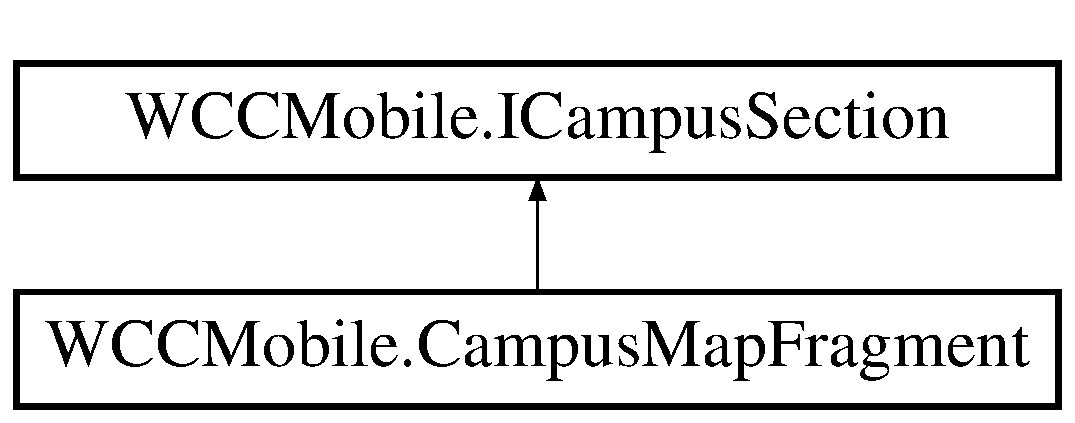
\includegraphics[height=2.000000cm]{interface_w_c_c_mobile_1_1_i_campus_section}
\end{center}
\end{figure}
\subsection*{Public Member Functions}
\begin{DoxyCompactItemize}
\item 
void {\bfseries Refresh\+Data} ()\hypertarget{interface_w_c_c_mobile_1_1_i_campus_section_a5ec794b8cf5fdab3f9d3829bb49d8a2d}{}\label{interface_w_c_c_mobile_1_1_i_campus_section_a5ec794b8cf5fdab3f9d3829bb49d8a2d}

\end{DoxyCompactItemize}
\subsection*{Properties}
\begin{DoxyCompactItemize}
\item 
string {\bfseries Name}\hspace{0.3cm}{\ttfamily  \mbox{[}get\mbox{]}}\hypertarget{interface_w_c_c_mobile_1_1_i_campus_section_ab3b480eb07b9a3870fbb6917e1f288f0}{}\label{interface_w_c_c_mobile_1_1_i_campus_section_ab3b480eb07b9a3870fbb6917e1f288f0}

\item 
string {\bfseries Title}\hspace{0.3cm}{\ttfamily  \mbox{[}get\mbox{]}}\hypertarget{interface_w_c_c_mobile_1_1_i_campus_section_a039503acb7ae09766b30bbd1fbedbad3}{}\label{interface_w_c_c_mobile_1_1_i_campus_section_a039503acb7ae09766b30bbd1fbedbad3}

\end{DoxyCompactItemize}


The documentation for this interface was generated from the following file\+:\begin{DoxyCompactItemize}
\item 
Source/\+Fragments/I\+Campus\+Section.\+cs\end{DoxyCompactItemize}

\hypertarget{class_w_c_c_mobile_1_1_resources_1_1_image_adapter}{}\section{W\+C\+C\+Mobile.\+Resources.\+Image\+Adapter Class Reference}
\label{class_w_c_c_mobile_1_1_resources_1_1_image_adapter}\index{W\+C\+C\+Mobile.\+Resources.\+Image\+Adapter@{W\+C\+C\+Mobile.\+Resources.\+Image\+Adapter}}
Inheritance diagram for W\+C\+C\+Mobile.\+Resources.\+Image\+Adapter\+:\begin{figure}[H]
\begin{center}
\leavevmode
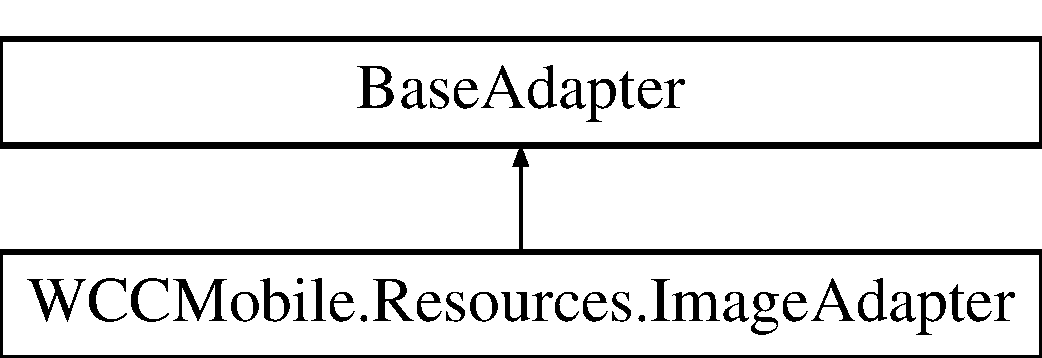
\includegraphics[height=2.000000cm]{class_w_c_c_mobile_1_1_resources_1_1_image_adapter}
\end{center}
\end{figure}
\subsection*{Public Member Functions}
\begin{DoxyCompactItemize}
\item 
\hyperlink{class_w_c_c_mobile_1_1_resources_1_1_image_adapter_aecdbda114f8bc3126786559cf2c07df9}{Image\+Adapter} (Context c)
\begin{DoxyCompactList}\small\item\em Initializes a new instance of the \hyperlink{class_w_c_c_mobile_1_1_resources_1_1_image_adapter}{Image\+Adapter} class. \end{DoxyCompactList}\item 
override Java.\+Lang.\+Object \hyperlink{class_w_c_c_mobile_1_1_resources_1_1_image_adapter_a5cd5bc1c3740deb80f83038b0acf2b8c}{Get\+Item} (int position)
\begin{DoxyCompactList}\small\item\em Gets the item. \end{DoxyCompactList}\item 
override long \hyperlink{class_w_c_c_mobile_1_1_resources_1_1_image_adapter_a3d2752b9736fd9110d594f1b445fd973}{Get\+Item\+Id} (int position)
\begin{DoxyCompactList}\small\item\em Gets the item identifier. \end{DoxyCompactList}\item 
override View \hyperlink{class_w_c_c_mobile_1_1_resources_1_1_image_adapter_a5584e8f229629bf756ba434b2834b2e1}{Get\+View} (int position, View convert\+View, View\+Group parent)
\begin{DoxyCompactList}\small\item\em Gets the view. \end{DoxyCompactList}\end{DoxyCompactItemize}
\subsection*{Properties}
\begin{DoxyCompactItemize}
\item 
override int \hyperlink{class_w_c_c_mobile_1_1_resources_1_1_image_adapter_a12551c76f768e8e243b2310f938ad1a5}{Count}\hspace{0.3cm}{\ttfamily  \mbox{[}get\mbox{]}}
\begin{DoxyCompactList}\small\item\em Gets the count. \end{DoxyCompactList}\item 
static int \hyperlink{class_w_c_c_mobile_1_1_resources_1_1_image_adapter_a27ed30bcea6fc0b4a0591373e4a3ae1a}{Label}\hspace{0.3cm}{\ttfamily  \mbox{[}get, set\mbox{]}}
\begin{DoxyCompactList}\small\item\em Gets or sets the label. \end{DoxyCompactList}\end{DoxyCompactItemize}


\subsection{Constructor \& Destructor Documentation}
\index{W\+C\+C\+Mobile\+::\+Resources\+::\+Image\+Adapter@{W\+C\+C\+Mobile\+::\+Resources\+::\+Image\+Adapter}!Image\+Adapter@{Image\+Adapter}}
\index{Image\+Adapter@{Image\+Adapter}!W\+C\+C\+Mobile\+::\+Resources\+::\+Image\+Adapter@{W\+C\+C\+Mobile\+::\+Resources\+::\+Image\+Adapter}}
\subsubsection[{\texorpdfstring{Image\+Adapter(\+Context c)}{ImageAdapter(Context c)}}]{\setlength{\rightskip}{0pt plus 5cm}W\+C\+C\+Mobile.\+Resources.\+Image\+Adapter.\+Image\+Adapter (
\begin{DoxyParamCaption}
\item[{Context}]{c}
\end{DoxyParamCaption}
)}\hypertarget{class_w_c_c_mobile_1_1_resources_1_1_image_adapter_aecdbda114f8bc3126786559cf2c07df9}{}\label{class_w_c_c_mobile_1_1_resources_1_1_image_adapter_aecdbda114f8bc3126786559cf2c07df9}


Initializes a new instance of the \hyperlink{class_w_c_c_mobile_1_1_resources_1_1_image_adapter}{Image\+Adapter} class. 


\begin{DoxyParams}{Parameters}
{\em c} & The c.\\
\hline
\end{DoxyParams}


\subsection{Member Function Documentation}
\index{W\+C\+C\+Mobile\+::\+Resources\+::\+Image\+Adapter@{W\+C\+C\+Mobile\+::\+Resources\+::\+Image\+Adapter}!Get\+Item@{Get\+Item}}
\index{Get\+Item@{Get\+Item}!W\+C\+C\+Mobile\+::\+Resources\+::\+Image\+Adapter@{W\+C\+C\+Mobile\+::\+Resources\+::\+Image\+Adapter}}
\subsubsection[{\texorpdfstring{Get\+Item(int position)}{GetItem(int position)}}]{\setlength{\rightskip}{0pt plus 5cm}override Java.\+Lang.\+Object W\+C\+C\+Mobile.\+Resources.\+Image\+Adapter.\+Get\+Item (
\begin{DoxyParamCaption}
\item[{int}]{position}
\end{DoxyParamCaption}
)}\hypertarget{class_w_c_c_mobile_1_1_resources_1_1_image_adapter_a5cd5bc1c3740deb80f83038b0acf2b8c}{}\label{class_w_c_c_mobile_1_1_resources_1_1_image_adapter_a5cd5bc1c3740deb80f83038b0acf2b8c}


Gets the item. 


\begin{DoxyParams}{Parameters}
{\em position} & The position.\\
\hline
\end{DoxyParams}
\begin{DoxyReturn}{Returns}

\end{DoxyReturn}
\index{W\+C\+C\+Mobile\+::\+Resources\+::\+Image\+Adapter@{W\+C\+C\+Mobile\+::\+Resources\+::\+Image\+Adapter}!Get\+Item\+Id@{Get\+Item\+Id}}
\index{Get\+Item\+Id@{Get\+Item\+Id}!W\+C\+C\+Mobile\+::\+Resources\+::\+Image\+Adapter@{W\+C\+C\+Mobile\+::\+Resources\+::\+Image\+Adapter}}
\subsubsection[{\texorpdfstring{Get\+Item\+Id(int position)}{GetItemId(int position)}}]{\setlength{\rightskip}{0pt plus 5cm}override long W\+C\+C\+Mobile.\+Resources.\+Image\+Adapter.\+Get\+Item\+Id (
\begin{DoxyParamCaption}
\item[{int}]{position}
\end{DoxyParamCaption}
)}\hypertarget{class_w_c_c_mobile_1_1_resources_1_1_image_adapter_a3d2752b9736fd9110d594f1b445fd973}{}\label{class_w_c_c_mobile_1_1_resources_1_1_image_adapter_a3d2752b9736fd9110d594f1b445fd973}


Gets the item identifier. 


\begin{DoxyParams}{Parameters}
{\em position} & The position.\\
\hline
\end{DoxyParams}
\begin{DoxyReturn}{Returns}

\end{DoxyReturn}
\index{W\+C\+C\+Mobile\+::\+Resources\+::\+Image\+Adapter@{W\+C\+C\+Mobile\+::\+Resources\+::\+Image\+Adapter}!Get\+View@{Get\+View}}
\index{Get\+View@{Get\+View}!W\+C\+C\+Mobile\+::\+Resources\+::\+Image\+Adapter@{W\+C\+C\+Mobile\+::\+Resources\+::\+Image\+Adapter}}
\subsubsection[{\texorpdfstring{Get\+View(int position, View convert\+View, View\+Group parent)}{GetView(int position, View convertView, ViewGroup parent)}}]{\setlength{\rightskip}{0pt plus 5cm}override View W\+C\+C\+Mobile.\+Resources.\+Image\+Adapter.\+Get\+View (
\begin{DoxyParamCaption}
\item[{int}]{position, }
\item[{View}]{convert\+View, }
\item[{View\+Group}]{parent}
\end{DoxyParamCaption}
)}\hypertarget{class_w_c_c_mobile_1_1_resources_1_1_image_adapter_a5584e8f229629bf756ba434b2834b2e1}{}\label{class_w_c_c_mobile_1_1_resources_1_1_image_adapter_a5584e8f229629bf756ba434b2834b2e1}


Gets the view. 


\begin{DoxyParams}{Parameters}
{\em position} & The position.\\
\hline
{\em convert\+View} & The convert view.\\
\hline
{\em parent} & The parent.\\
\hline
\end{DoxyParams}
\begin{DoxyReturn}{Returns}

\end{DoxyReturn}


\subsection{Property Documentation}
\index{W\+C\+C\+Mobile\+::\+Resources\+::\+Image\+Adapter@{W\+C\+C\+Mobile\+::\+Resources\+::\+Image\+Adapter}!Count@{Count}}
\index{Count@{Count}!W\+C\+C\+Mobile\+::\+Resources\+::\+Image\+Adapter@{W\+C\+C\+Mobile\+::\+Resources\+::\+Image\+Adapter}}
\subsubsection[{\texorpdfstring{Count}{Count}}]{\setlength{\rightskip}{0pt plus 5cm}override int W\+C\+C\+Mobile.\+Resources.\+Image\+Adapter.\+Count\hspace{0.3cm}{\ttfamily [get]}}\hypertarget{class_w_c_c_mobile_1_1_resources_1_1_image_adapter_a12551c76f768e8e243b2310f938ad1a5}{}\label{class_w_c_c_mobile_1_1_resources_1_1_image_adapter_a12551c76f768e8e243b2310f938ad1a5}


Gets the count. 

The count. \index{W\+C\+C\+Mobile\+::\+Resources\+::\+Image\+Adapter@{W\+C\+C\+Mobile\+::\+Resources\+::\+Image\+Adapter}!Label@{Label}}
\index{Label@{Label}!W\+C\+C\+Mobile\+::\+Resources\+::\+Image\+Adapter@{W\+C\+C\+Mobile\+::\+Resources\+::\+Image\+Adapter}}
\subsubsection[{\texorpdfstring{Label}{Label}}]{\setlength{\rightskip}{0pt plus 5cm}int W\+C\+C\+Mobile.\+Resources.\+Image\+Adapter.\+Label\hspace{0.3cm}{\ttfamily [static]}, {\ttfamily [get]}, {\ttfamily [set]}}\hypertarget{class_w_c_c_mobile_1_1_resources_1_1_image_adapter_a27ed30bcea6fc0b4a0591373e4a3ae1a}{}\label{class_w_c_c_mobile_1_1_resources_1_1_image_adapter_a27ed30bcea6fc0b4a0591373e4a3ae1a}


Gets or sets the label. 

The label. 

The documentation for this class was generated from the following file\+:\begin{DoxyCompactItemize}
\item 
Source/\+Adapters/Image\+Adapter.\+cs\end{DoxyCompactItemize}

\hypertarget{class_w_c_c_mobile_1_1_info_bar_controller}{}\section{W\+C\+C\+Mobile.\+Info\+Bar\+Controller Class Reference}
\label{class_w_c_c_mobile_1_1_info_bar_controller}\index{W\+C\+C\+Mobile.\+Info\+Bar\+Controller@{W\+C\+C\+Mobile.\+Info\+Bar\+Controller}}
\subsection*{Public Member Functions}
\begin{DoxyCompactItemize}
\item 
{\bfseries Info\+Bar\+Controller} (View parent\+View)\hypertarget{class_w_c_c_mobile_1_1_info_bar_controller_abbcd4a83b1ac3c04d42f1711080e37d7}{}\label{class_w_c_c_mobile_1_1_info_bar_controller_abbcd4a83b1ac3c04d42f1711080e37d7}

\item 
void {\bfseries Show\+Loading} ()\hypertarget{class_w_c_c_mobile_1_1_info_bar_controller_a182c560ef03faf572837bbdef759bdbc}{}\label{class_w_c_c_mobile_1_1_info_bar_controller_a182c560ef03faf572837bbdef759bdbc}

\item 
void {\bfseries Show\+Loaded} ()\hypertarget{class_w_c_c_mobile_1_1_info_bar_controller_a8d66dad968254e4c960f642d655ac332}{}\label{class_w_c_c_mobile_1_1_info_bar_controller_a8d66dad968254e4c960f642d655ac332}

\item 
void {\bfseries Show\+Information} (string info)\hypertarget{class_w_c_c_mobile_1_1_info_bar_controller_aa74dd49a96e71c6a87476755c4a58709}{}\label{class_w_c_c_mobile_1_1_info_bar_controller_aa74dd49a96e71c6a87476755c4a58709}

\end{DoxyCompactItemize}


The documentation for this class was generated from the following file\+:\begin{DoxyCompactItemize}
\item 
Source/\+Controls/Info\+Bar\+Controller.\+cs\end{DoxyCompactItemize}

\hypertarget{class_w_c_c_mobile_1_1_info_pane}{}\section{W\+C\+C\+Mobile.\+Info\+Pane Class Reference}
\label{class_w_c_c_mobile_1_1_info_pane}\index{W\+C\+C\+Mobile.\+Info\+Pane@{W\+C\+C\+Mobile.\+Info\+Pane}}
Inheritance diagram for W\+C\+C\+Mobile.\+Info\+Pane\+:\begin{figure}[H]
\begin{center}
\leavevmode
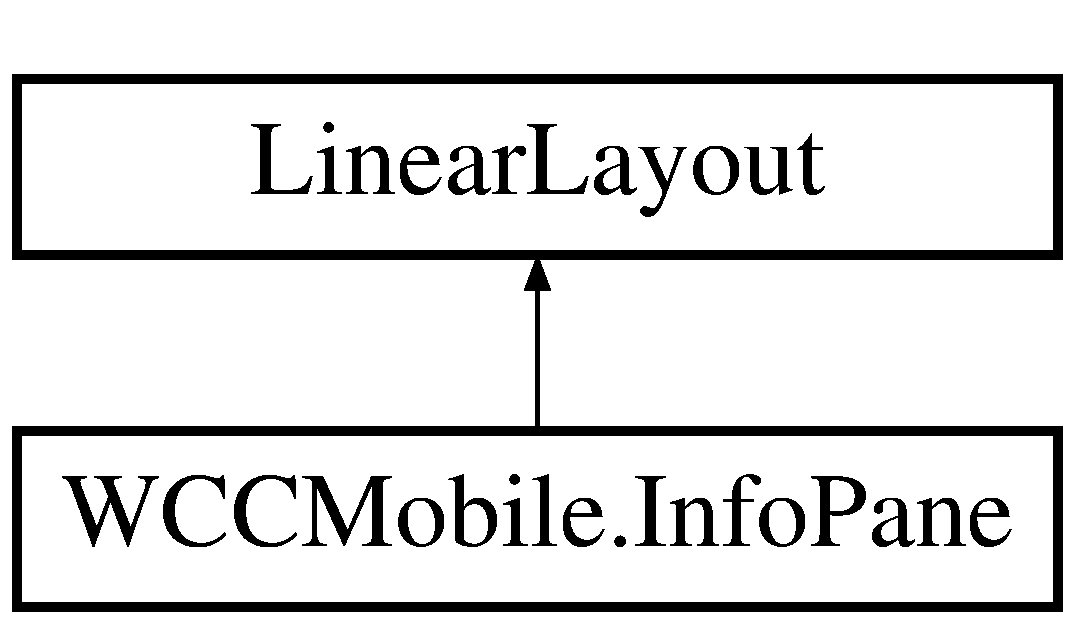
\includegraphics[height=2.000000cm]{class_w_c_c_mobile_1_1_info_pane}
\end{center}
\end{figure}
\subsection*{Public Types}
\begin{DoxyCompactItemize}
\item 
enum {\bfseries State} \{ {\bfseries Closed}, 
{\bfseries Opened}, 
{\bfseries Fully\+Opened}
 \}\hypertarget{class_w_c_c_mobile_1_1_info_pane_a771339a51702ed505cd36b8c973c5153}{}\label{class_w_c_c_mobile_1_1_info_pane_a771339a51702ed505cd36b8c973c5153}

\end{DoxyCompactItemize}
\subsection*{Public Member Functions}
\begin{DoxyCompactItemize}
\item 
\hyperlink{class_w_c_c_mobile_1_1_info_pane_ae925e23fa98234101c549cc9a038503d}{Info\+Pane} (Context context)
\begin{DoxyCompactList}\small\item\em Initializes a new instance of the \hyperlink{class_w_c_c_mobile_1_1_info_pane}{Info\+Pane} class. \end{DoxyCompactList}\item 
\hyperlink{class_w_c_c_mobile_1_1_info_pane_a36d1b1d35905f3ae02cf64f791c54349}{Info\+Pane} (Context context, I\+Attribute\+Set attrs)
\begin{DoxyCompactList}\small\item\em Initializes a new instance of the \hyperlink{class_w_c_c_mobile_1_1_info_pane}{Info\+Pane} class. \end{DoxyCompactList}\item 
\hyperlink{class_w_c_c_mobile_1_1_info_pane_af14668954e11cc545a5d63aa6787e73c}{Info\+Pane} (Context context, I\+Attribute\+Set attrs, int def\+Style)
\begin{DoxyCompactList}\small\item\em Initializes a new instance of the \hyperlink{class_w_c_c_mobile_1_1_info_pane}{Info\+Pane} class. \end{DoxyCompactList}\item 
void \hyperlink{class_w_c_c_mobile_1_1_info_pane_a236327622ae5c4d3b3725a0d3ebd880a}{Set\+State} (State new\+State, bool animated=true)
\begin{DoxyCompactList}\small\item\em Sets the state of this instance of \hyperlink{class_w_c_c_mobile_1_1_info_pane}{Info\+Pane} offset status. \end{DoxyCompactList}\item 
override bool \hyperlink{class_w_c_c_mobile_1_1_info_pane_a30c1c1fb3ecea8f9a2c2f8b7c7c0cadf}{On\+Touch\+Event} (Motion\+Event e)
\begin{DoxyCompactList}\small\item\em Called when \mbox{[}touch event\mbox{]}. \end{DoxyCompactList}\end{DoxyCompactItemize}
\subsection*{Protected Member Functions}
\begin{DoxyCompactItemize}
\item 
override void \hyperlink{class_w_c_c_mobile_1_1_info_pane_a618d2d1015417dfef2664c42b0c37ff1}{Dispatch\+Draw} (Android.\+Graphics.\+Canvas canvas)
\begin{DoxyCompactList}\small\item\em Dispatches the draw. \end{DoxyCompactList}\end{DoxyCompactItemize}
\subsection*{Properties}
\begin{DoxyCompactItemize}
\item 
bool \hyperlink{class_w_c_c_mobile_1_1_info_pane_a531dc065a09acf3e692f91f9620bc010}{Opened}\hspace{0.3cm}{\ttfamily  \mbox{[}get\mbox{]}}
\begin{DoxyCompactList}\small\item\em Gets a value indicating whether this \hyperlink{class_w_c_c_mobile_1_1_info_pane}{Info\+Pane} is opened. \end{DoxyCompactList}\item 
bool \hyperlink{class_w_c_c_mobile_1_1_info_pane_afedca359f93cda198f4b1b0d59c187d9}{Fully\+Opened}\hspace{0.3cm}{\ttfamily  \mbox{[}get\mbox{]}}
\begin{DoxyCompactList}\small\item\em Gets a value indicating whether \mbox{[}fully opened\mbox{]}. \end{DoxyCompactList}\end{DoxyCompactItemize}
\subsection*{Events}
\begin{DoxyCompactItemize}
\item 
Action$<$ State $>$ {\bfseries State\+Changed}\hypertarget{class_w_c_c_mobile_1_1_info_pane_a38144d3db3575dce5322a154f4a20c08}{}\label{class_w_c_c_mobile_1_1_info_pane_a38144d3db3575dce5322a154f4a20c08}

\end{DoxyCompactItemize}


\subsection{Constructor \& Destructor Documentation}
\index{W\+C\+C\+Mobile\+::\+Info\+Pane@{W\+C\+C\+Mobile\+::\+Info\+Pane}!Info\+Pane@{Info\+Pane}}
\index{Info\+Pane@{Info\+Pane}!W\+C\+C\+Mobile\+::\+Info\+Pane@{W\+C\+C\+Mobile\+::\+Info\+Pane}}
\subsubsection[{\texorpdfstring{Info\+Pane(\+Context context)}{InfoPane(Context context)}}]{\setlength{\rightskip}{0pt plus 5cm}W\+C\+C\+Mobile.\+Info\+Pane.\+Info\+Pane (
\begin{DoxyParamCaption}
\item[{Context}]{context}
\end{DoxyParamCaption}
)}\hypertarget{class_w_c_c_mobile_1_1_info_pane_ae925e23fa98234101c549cc9a038503d}{}\label{class_w_c_c_mobile_1_1_info_pane_ae925e23fa98234101c549cc9a038503d}


Initializes a new instance of the \hyperlink{class_w_c_c_mobile_1_1_info_pane}{Info\+Pane} class. 


\begin{DoxyParams}{Parameters}
{\em context} & The context.\\
\hline
\end{DoxyParams}
\index{W\+C\+C\+Mobile\+::\+Info\+Pane@{W\+C\+C\+Mobile\+::\+Info\+Pane}!Info\+Pane@{Info\+Pane}}
\index{Info\+Pane@{Info\+Pane}!W\+C\+C\+Mobile\+::\+Info\+Pane@{W\+C\+C\+Mobile\+::\+Info\+Pane}}
\subsubsection[{\texorpdfstring{Info\+Pane(\+Context context, I\+Attribute\+Set attrs)}{InfoPane(Context context, IAttributeSet attrs)}}]{\setlength{\rightskip}{0pt plus 5cm}W\+C\+C\+Mobile.\+Info\+Pane.\+Info\+Pane (
\begin{DoxyParamCaption}
\item[{Context}]{context, }
\item[{I\+Attribute\+Set}]{attrs}
\end{DoxyParamCaption}
)}\hypertarget{class_w_c_c_mobile_1_1_info_pane_a36d1b1d35905f3ae02cf64f791c54349}{}\label{class_w_c_c_mobile_1_1_info_pane_a36d1b1d35905f3ae02cf64f791c54349}


Initializes a new instance of the \hyperlink{class_w_c_c_mobile_1_1_info_pane}{Info\+Pane} class. 


\begin{DoxyParams}{Parameters}
{\em context} & The context.\\
\hline
{\em attrs} & The attrs.\\
\hline
\end{DoxyParams}
\index{W\+C\+C\+Mobile\+::\+Info\+Pane@{W\+C\+C\+Mobile\+::\+Info\+Pane}!Info\+Pane@{Info\+Pane}}
\index{Info\+Pane@{Info\+Pane}!W\+C\+C\+Mobile\+::\+Info\+Pane@{W\+C\+C\+Mobile\+::\+Info\+Pane}}
\subsubsection[{\texorpdfstring{Info\+Pane(\+Context context, I\+Attribute\+Set attrs, int def\+Style)}{InfoPane(Context context, IAttributeSet attrs, int defStyle)}}]{\setlength{\rightskip}{0pt plus 5cm}W\+C\+C\+Mobile.\+Info\+Pane.\+Info\+Pane (
\begin{DoxyParamCaption}
\item[{Context}]{context, }
\item[{I\+Attribute\+Set}]{attrs, }
\item[{int}]{def\+Style}
\end{DoxyParamCaption}
)}\hypertarget{class_w_c_c_mobile_1_1_info_pane_af14668954e11cc545a5d63aa6787e73c}{}\label{class_w_c_c_mobile_1_1_info_pane_af14668954e11cc545a5d63aa6787e73c}


Initializes a new instance of the \hyperlink{class_w_c_c_mobile_1_1_info_pane}{Info\+Pane} class. 


\begin{DoxyParams}{Parameters}
{\em context} & The context.\\
\hline
{\em attrs} & The attrs.\\
\hline
{\em def\+Style} & The definition style.\\
\hline
\end{DoxyParams}


\subsection{Member Function Documentation}
\index{W\+C\+C\+Mobile\+::\+Info\+Pane@{W\+C\+C\+Mobile\+::\+Info\+Pane}!Dispatch\+Draw@{Dispatch\+Draw}}
\index{Dispatch\+Draw@{Dispatch\+Draw}!W\+C\+C\+Mobile\+::\+Info\+Pane@{W\+C\+C\+Mobile\+::\+Info\+Pane}}
\subsubsection[{\texorpdfstring{Dispatch\+Draw(\+Android.\+Graphics.\+Canvas canvas)}{DispatchDraw(Android.Graphics.Canvas canvas)}}]{\setlength{\rightskip}{0pt plus 5cm}override void W\+C\+C\+Mobile.\+Info\+Pane.\+Dispatch\+Draw (
\begin{DoxyParamCaption}
\item[{Android.\+Graphics.\+Canvas}]{canvas}
\end{DoxyParamCaption}
)\hspace{0.3cm}{\ttfamily [protected]}}\hypertarget{class_w_c_c_mobile_1_1_info_pane_a618d2d1015417dfef2664c42b0c37ff1}{}\label{class_w_c_c_mobile_1_1_info_pane_a618d2d1015417dfef2664c42b0c37ff1}


Dispatches the draw. 


\begin{DoxyParams}{Parameters}
{\em canvas} & The canvas.\\
\hline
\end{DoxyParams}
\index{W\+C\+C\+Mobile\+::\+Info\+Pane@{W\+C\+C\+Mobile\+::\+Info\+Pane}!On\+Touch\+Event@{On\+Touch\+Event}}
\index{On\+Touch\+Event@{On\+Touch\+Event}!W\+C\+C\+Mobile\+::\+Info\+Pane@{W\+C\+C\+Mobile\+::\+Info\+Pane}}
\subsubsection[{\texorpdfstring{On\+Touch\+Event(\+Motion\+Event e)}{OnTouchEvent(MotionEvent e)}}]{\setlength{\rightskip}{0pt plus 5cm}override bool W\+C\+C\+Mobile.\+Info\+Pane.\+On\+Touch\+Event (
\begin{DoxyParamCaption}
\item[{Motion\+Event}]{e}
\end{DoxyParamCaption}
)}\hypertarget{class_w_c_c_mobile_1_1_info_pane_a30c1c1fb3ecea8f9a2c2f8b7c7c0cadf}{}\label{class_w_c_c_mobile_1_1_info_pane_a30c1c1fb3ecea8f9a2c2f8b7c7c0cadf}


Called when \mbox{[}touch event\mbox{]}. 


\begin{DoxyParams}{Parameters}
{\em e} & The e.\\
\hline
\end{DoxyParams}
\begin{DoxyReturn}{Returns}

\end{DoxyReturn}
\index{W\+C\+C\+Mobile\+::\+Info\+Pane@{W\+C\+C\+Mobile\+::\+Info\+Pane}!Set\+State@{Set\+State}}
\index{Set\+State@{Set\+State}!W\+C\+C\+Mobile\+::\+Info\+Pane@{W\+C\+C\+Mobile\+::\+Info\+Pane}}
\subsubsection[{\texorpdfstring{Set\+State(\+State new\+State, bool animated=true)}{SetState(State newState, bool animated=true)}}]{\setlength{\rightskip}{0pt plus 5cm}void W\+C\+C\+Mobile.\+Info\+Pane.\+Set\+State (
\begin{DoxyParamCaption}
\item[{State}]{new\+State, }
\item[{bool}]{animated = {\ttfamily true}}
\end{DoxyParamCaption}
)}\hypertarget{class_w_c_c_mobile_1_1_info_pane_a236327622ae5c4d3b3725a0d3ebd880a}{}\label{class_w_c_c_mobile_1_1_info_pane_a236327622ae5c4d3b3725a0d3ebd880a}


Sets the state of this instance of \hyperlink{class_w_c_c_mobile_1_1_info_pane}{Info\+Pane} offset status. 


\begin{DoxyParams}{Parameters}
{\em new\+State} & The new state.\\
\hline
{\em animated} & if set to {\ttfamily true} \mbox{[}animated\mbox{]}.\\
\hline
\end{DoxyParams}


\subsection{Property Documentation}
\index{W\+C\+C\+Mobile\+::\+Info\+Pane@{W\+C\+C\+Mobile\+::\+Info\+Pane}!Fully\+Opened@{Fully\+Opened}}
\index{Fully\+Opened@{Fully\+Opened}!W\+C\+C\+Mobile\+::\+Info\+Pane@{W\+C\+C\+Mobile\+::\+Info\+Pane}}
\subsubsection[{\texorpdfstring{Fully\+Opened}{FullyOpened}}]{\setlength{\rightskip}{0pt plus 5cm}bool W\+C\+C\+Mobile.\+Info\+Pane.\+Fully\+Opened\hspace{0.3cm}{\ttfamily [get]}}\hypertarget{class_w_c_c_mobile_1_1_info_pane_afedca359f93cda198f4b1b0d59c187d9}{}\label{class_w_c_c_mobile_1_1_info_pane_afedca359f93cda198f4b1b0d59c187d9}


Gets a value indicating whether \mbox{[}fully opened\mbox{]}. 

{\ttfamily true} if \mbox{[}fully opened\mbox{]}; otherwise, {\ttfamily false}. \index{W\+C\+C\+Mobile\+::\+Info\+Pane@{W\+C\+C\+Mobile\+::\+Info\+Pane}!Opened@{Opened}}
\index{Opened@{Opened}!W\+C\+C\+Mobile\+::\+Info\+Pane@{W\+C\+C\+Mobile\+::\+Info\+Pane}}
\subsubsection[{\texorpdfstring{Opened}{Opened}}]{\setlength{\rightskip}{0pt plus 5cm}bool W\+C\+C\+Mobile.\+Info\+Pane.\+Opened\hspace{0.3cm}{\ttfamily [get]}}\hypertarget{class_w_c_c_mobile_1_1_info_pane_a531dc065a09acf3e692f91f9620bc010}{}\label{class_w_c_c_mobile_1_1_info_pane_a531dc065a09acf3e692f91f9620bc010}


Gets a value indicating whether this \hyperlink{class_w_c_c_mobile_1_1_info_pane}{Info\+Pane} is opened. 

{\ttfamily true} if opened; otherwise, {\ttfamily false}. 

The documentation for this class was generated from the following file\+:\begin{DoxyCompactItemize}
\item 
Source/\+Controls/Info\+Pane.\+cs\end{DoxyCompactItemize}

\hypertarget{struct_w_c_c_mobile_1_1_location}{}\section{W\+C\+C\+Mobile.\+Location Struct Reference}
\label{struct_w_c_c_mobile_1_1_location}\index{W\+C\+C\+Mobile.\+Location@{W\+C\+C\+Mobile.\+Location}}
\subsection*{Properties}
\begin{DoxyCompactItemize}
\item 
bool {\bfseries Init}\hspace{0.3cm}{\ttfamily  \mbox{[}get, set\mbox{]}}\hypertarget{struct_w_c_c_mobile_1_1_location_a5ab2e1f144bdae43a9bbb6bb899ccc55}{}\label{struct_w_c_c_mobile_1_1_location_a5ab2e1f144bdae43a9bbb6bb899ccc55}

\item 
double {\bfseries Lat}\hspace{0.3cm}{\ttfamily  \mbox{[}get, set\mbox{]}}\hypertarget{struct_w_c_c_mobile_1_1_location_a9fc5eb7b6baa78f6165c9fa9ea229482}{}\label{struct_w_c_c_mobile_1_1_location_a9fc5eb7b6baa78f6165c9fa9ea229482}

\item 
double {\bfseries Lon}\hspace{0.3cm}{\ttfamily  \mbox{[}get, set\mbox{]}}\hypertarget{struct_w_c_c_mobile_1_1_location_a32e729302f213d15df7bb0c8c6cb3767}{}\label{struct_w_c_c_mobile_1_1_location_a32e729302f213d15df7bb0c8c6cb3767}

\end{DoxyCompactItemize}


The documentation for this struct was generated from the following file\+:\begin{DoxyCompactItemize}
\item 
Source/\+Models/Location.\+cs\end{DoxyCompactItemize}

\hypertarget{class_w_c_c_mobile_1_1_location_utils}{}\section{W\+C\+C\+Mobile.\+Location\+Utils Class Reference}
\label{class_w_c_c_mobile_1_1_location_utils}\index{W\+C\+C\+Mobile.\+Location\+Utils@{W\+C\+C\+Mobile.\+Location\+Utils}}
\subsection*{Static Public Member Functions}
\begin{DoxyCompactItemize}
\item 
static double \hyperlink{class_w_c_c_mobile_1_1_location_utils_a2dece4c8bb1149688a0724e6a91ff39b}{Distance} (\hyperlink{struct_w_c_c_mobile_1_1_location}{Location} p1, \hyperlink{struct_w_c_c_mobile_1_1_location}{Location} p2)
\begin{DoxyCompactList}\small\item\em Calculates the geodesic between {\itshape p1}  and {\itshape p2}  using law of cosines. \end{DoxyCompactList}\item 
static void \hyperlink{class_w_c_c_mobile_1_1_location_utils_aced59b8c81cbeed0cbf0818add183418}{Dump\+Location} (\hyperlink{struct_w_c_c_mobile_1_1_location}{Location} p, Stream stream)
\begin{DoxyCompactList}\small\item\em writes the location using Binary\+Writer. \end{DoxyCompactList}\item 
static \hyperlink{struct_w_c_c_mobile_1_1_location}{Location} \hyperlink{class_w_c_c_mobile_1_1_location_utils_a2ca1849312e2cf045c77750043a2fe58}{Parse\+From\+Stream} (Stream stream)
\begin{DoxyCompactList}\small\item\em Parses the location from stream. \end{DoxyCompactList}\end{DoxyCompactItemize}


\subsection{Member Function Documentation}
\index{W\+C\+C\+Mobile\+::\+Location\+Utils@{W\+C\+C\+Mobile\+::\+Location\+Utils}!Distance@{Distance}}
\index{Distance@{Distance}!W\+C\+C\+Mobile\+::\+Location\+Utils@{W\+C\+C\+Mobile\+::\+Location\+Utils}}
\subsubsection[{\texorpdfstring{Distance(\+Location p1, Location p2)}{Distance(Location p1, Location p2)}}]{\setlength{\rightskip}{0pt plus 5cm}static double W\+C\+C\+Mobile.\+Location\+Utils.\+Distance (
\begin{DoxyParamCaption}
\item[{{\bf Location}}]{p1, }
\item[{{\bf Location}}]{p2}
\end{DoxyParamCaption}
)\hspace{0.3cm}{\ttfamily [static]}}\hypertarget{class_w_c_c_mobile_1_1_location_utils_a2dece4c8bb1149688a0724e6a91ff39b}{}\label{class_w_c_c_mobile_1_1_location_utils_a2dece4c8bb1149688a0724e6a91ff39b}


Calculates the geodesic between {\itshape p1}  and {\itshape p2}  using law of cosines. 


\begin{DoxyParams}{Parameters}
{\em p1} & The p1.\\
\hline
{\em p2} & The p2.\\
\hline
\end{DoxyParams}
\begin{DoxyReturn}{Returns}

\end{DoxyReturn}
\index{W\+C\+C\+Mobile\+::\+Location\+Utils@{W\+C\+C\+Mobile\+::\+Location\+Utils}!Dump\+Location@{Dump\+Location}}
\index{Dump\+Location@{Dump\+Location}!W\+C\+C\+Mobile\+::\+Location\+Utils@{W\+C\+C\+Mobile\+::\+Location\+Utils}}
\subsubsection[{\texorpdfstring{Dump\+Location(\+Location p, Stream stream)}{DumpLocation(Location p, Stream stream)}}]{\setlength{\rightskip}{0pt plus 5cm}static void W\+C\+C\+Mobile.\+Location\+Utils.\+Dump\+Location (
\begin{DoxyParamCaption}
\item[{{\bf Location}}]{p, }
\item[{Stream}]{stream}
\end{DoxyParamCaption}
)\hspace{0.3cm}{\ttfamily [static]}}\hypertarget{class_w_c_c_mobile_1_1_location_utils_aced59b8c81cbeed0cbf0818add183418}{}\label{class_w_c_c_mobile_1_1_location_utils_aced59b8c81cbeed0cbf0818add183418}


writes the location using Binary\+Writer. 


\begin{DoxyParams}{Parameters}
{\em p} & The p.\\
\hline
{\em stream} & The stream.\\
\hline
\end{DoxyParams}
\index{W\+C\+C\+Mobile\+::\+Location\+Utils@{W\+C\+C\+Mobile\+::\+Location\+Utils}!Parse\+From\+Stream@{Parse\+From\+Stream}}
\index{Parse\+From\+Stream@{Parse\+From\+Stream}!W\+C\+C\+Mobile\+::\+Location\+Utils@{W\+C\+C\+Mobile\+::\+Location\+Utils}}
\subsubsection[{\texorpdfstring{Parse\+From\+Stream(\+Stream stream)}{ParseFromStream(Stream stream)}}]{\setlength{\rightskip}{0pt plus 5cm}static {\bf Location} W\+C\+C\+Mobile.\+Location\+Utils.\+Parse\+From\+Stream (
\begin{DoxyParamCaption}
\item[{Stream}]{stream}
\end{DoxyParamCaption}
)\hspace{0.3cm}{\ttfamily [static]}}\hypertarget{class_w_c_c_mobile_1_1_location_utils_a2ca1849312e2cf045c77750043a2fe58}{}\label{class_w_c_c_mobile_1_1_location_utils_a2ca1849312e2cf045c77750043a2fe58}


Parses the location from stream. 


\begin{DoxyParams}{Parameters}
{\em stream} & The stream.\\
\hline
\end{DoxyParams}
\begin{DoxyReturn}{Returns}

\end{DoxyReturn}


The documentation for this class was generated from the following file\+:\begin{DoxyCompactItemize}
\item 
Source/\+Helpers/Location\+Utils.\+cs\end{DoxyCompactItemize}

\hypertarget{class_w_c_c_mobile_1_1_l_r_u_cache}{}\section{W\+C\+C\+Mobile.\+L\+R\+U\+Cache$<$ T\+Key, T\+Value $>$ Class Template Reference}
\label{class_w_c_c_mobile_1_1_l_r_u_cache}\index{W\+C\+C\+Mobile.\+L\+R\+U\+Cache$<$ T\+Key, T\+Value $>$@{W\+C\+C\+Mobile.\+L\+R\+U\+Cache$<$ T\+Key, T\+Value $>$}}
\subsection*{Public Member Functions}
\begin{DoxyCompactItemize}
\item 
{\bfseries L\+R\+U\+Cache} (int capacity)\hypertarget{class_w_c_c_mobile_1_1_l_r_u_cache_a3dbc0f5ae542b6def7914f7edcfd943d}{}\label{class_w_c_c_mobile_1_1_l_r_u_cache_a3dbc0f5ae542b6def7914f7edcfd943d}

\item 
void {\bfseries Put} (T\+Key key, T\+Value value)\hypertarget{class_w_c_c_mobile_1_1_l_r_u_cache_a596c1634fd7f0359e87ed983b77a1dfc}{}\label{class_w_c_c_mobile_1_1_l_r_u_cache_a596c1634fd7f0359e87ed983b77a1dfc}

\item 
T\+Value {\bfseries Get} (T\+Key key)\hypertarget{class_w_c_c_mobile_1_1_l_r_u_cache_aeb62fa6c77765944733cd3cc2c94cd33}{}\label{class_w_c_c_mobile_1_1_l_r_u_cache_aeb62fa6c77765944733cd3cc2c94cd33}

\end{DoxyCompactItemize}


The documentation for this class was generated from the following file\+:\begin{DoxyCompactItemize}
\item 
Source/\+Storage/L\+R\+U\+Cache.\+cs\end{DoxyCompactItemize}

\hypertarget{class_w_c_c_mobile_1_1_main_activity}{}\section{W\+C\+C\+Mobile.\+Main\+Activity Class Reference}
\label{class_w_c_c_mobile_1_1_main_activity}\index{W\+C\+C\+Mobile.\+Main\+Activity@{W\+C\+C\+Mobile.\+Main\+Activity}}
Inheritance diagram for W\+C\+C\+Mobile.\+Main\+Activity\+:\begin{figure}[H]
\begin{center}
\leavevmode
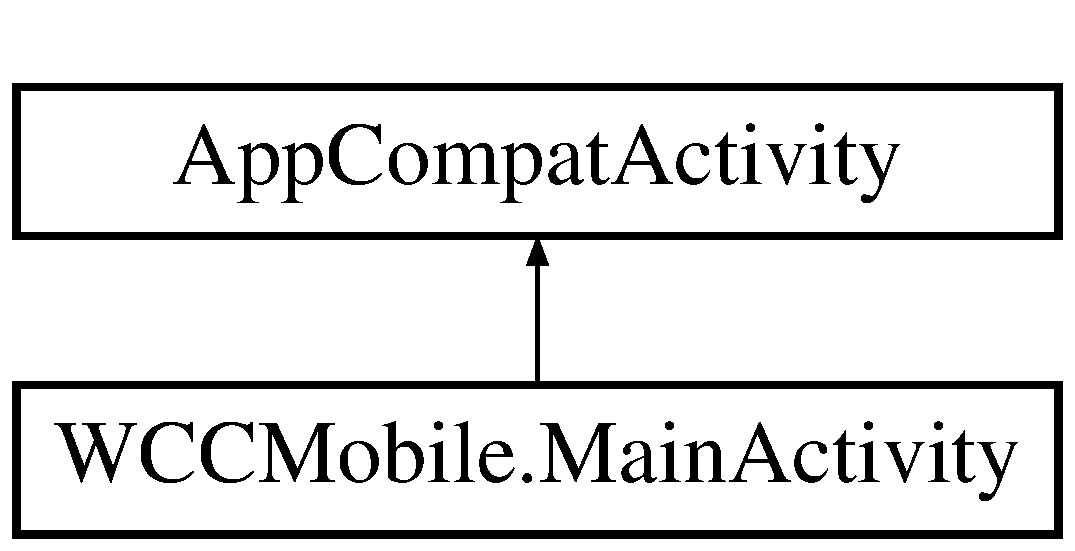
\includegraphics[height=2.000000cm]{class_w_c_c_mobile_1_1_main_activity}
\end{center}
\end{figure}
\subsection*{Public Member Functions}
\begin{DoxyCompactItemize}
\item 
void \hyperlink{class_w_c_c_mobile_1_1_main_activity_accc284f1d0d4e2ae045db80981c51bc8}{Do\+Work} ()
\begin{DoxyCompactList}\small\item\em Does the work. \end{DoxyCompactList}\item 
void \hyperlink{class_w_c_c_mobile_1_1_main_activity_a9505a34d42917317eff31a4e7872b7d6}{Alert\+Not\+Implemented} ()
\begin{DoxyCompactList}\small\item\em Alerts the not implemented. \end{DoxyCompactList}\item 
override void \hyperlink{class_w_c_c_mobile_1_1_main_activity_a6d31456aafea0e368a6899dbb2c81ae2}{On\+Back\+Pressed} ()
\begin{DoxyCompactList}\small\item\em Called when the activity has detected the user\textquotesingle{}s press of the back key. \end{DoxyCompactList}\item 
string \hyperlink{class_w_c_c_mobile_1_1_main_activity_a58c410fc67bdc0feb2d8130f55fa4948}{get\+H\+T\+ML} (string url=\char`\"{}http\+://www.\+sunywcc.\+edu/\char`\"{})
\begin{DoxyCompactList}\small\item\em Gets the H\+T\+ML. \end{DoxyCompactList}\end{DoxyCompactItemize}
\subsection*{Static Public Member Functions}
\begin{DoxyCompactItemize}
\item 
static void \hyperlink{class_w_c_c_mobile_1_1_main_activity_af8be63bdc0157ababa092069a770d679}{Start\+Sub\+App} (int args)
\begin{DoxyCompactList}\small\item\em Starts the sub application. \end{DoxyCompactList}\item 
static void \hyperlink{class_w_c_c_mobile_1_1_main_activity_a9ac2a808a8655ab4bab6de5a954f277f}{Start\+External\+App} (string app\+Package\+Name, Activity Caller)
\begin{DoxyCompactList}\small\item\em Can be used by any sub App to launch external 3rd Party apps pass the Activity that wishes to launch and the package name to get the package name search the app name on \+: \href{http://apk-dl.com/}{\tt http\+://apk-\/dl.\+com/} \end{DoxyCompactList}\end{DoxyCompactItemize}
\subsection*{Public Attributes}
\begin{DoxyCompactItemize}
\item 
Grid\+View {\bfseries Sub\+App\+Container}\hypertarget{class_w_c_c_mobile_1_1_main_activity_a8918397ea1a62b7847adb444381f63d0}{}\label{class_w_c_c_mobile_1_1_main_activity_a8918397ea1a62b7847adb444381f63d0}

\end{DoxyCompactItemize}
\subsection*{Static Public Attributes}
\begin{DoxyCompactItemize}
\item 
static Image\+View {\bfseries Image\+Container}\hypertarget{class_w_c_c_mobile_1_1_main_activity_a1f6b73d0f45d54348e90a3e42196f93b}{}\label{class_w_c_c_mobile_1_1_main_activity_a1f6b73d0f45d54348e90a3e42196f93b}

\item 
static readonly Random \hyperlink{class_w_c_c_mobile_1_1_main_activity_afcfd9d936ed9d4ebd09e620e7643bb2f}{L\+O\+KI} = new Random()
\begin{DoxyCompactList}\small\item\em The random number generator. \end{DoxyCompactList}\end{DoxyCompactItemize}
\subsection*{Protected Member Functions}
\begin{DoxyCompactItemize}
\item 
override void \hyperlink{class_w_c_c_mobile_1_1_main_activity_a2fe5821eafde95e4c73e3f548a83cce2}{On\+Create} (Bundle bundle)
\begin{DoxyCompactList}\small\item\em Called when \mbox{[}create\mbox{]}. \end{DoxyCompactList}\item 
override void \hyperlink{class_w_c_c_mobile_1_1_main_activity_ae1bcf5ddd333e0f1fde16e9219549448}{On\+Start} ()
\begin{DoxyCompactList}\small\item\em Called after On\+Create and Also when a Subb\+App closes -\/ resets is\+Ready \end{DoxyCompactList}\end{DoxyCompactItemize}
\subsection*{Properties}
\begin{DoxyCompactItemize}
\item 
static \hyperlink{class_w_c_c_mobile_1_1_main_activity}{Main\+Activity} \hyperlink{class_w_c_c_mobile_1_1_main_activity_aabc36edadb3768e48df7834bc7204f8e}{singleR}\hspace{0.3cm}{\ttfamily  \mbox{[}get\mbox{]}}
\begin{DoxyCompactList}\small\item\em Gets the singleton instance of the \hyperlink{class_w_c_c_mobile_1_1_main_activity}{Main\+Activity}. \end{DoxyCompactList}\item 
static bool \hyperlink{class_w_c_c_mobile_1_1_main_activity_a392159539f2848512f11189310be9280}{is\+Ready}\hspace{0.3cm}{\ttfamily  \mbox{[}get, set\mbox{]}}
\begin{DoxyCompactList}\small\item\em Gets or sets a value indicating whether this instance is ready. \end{DoxyCompactList}\item 
static System.\+Collections.\+Generic.\+List$<$ Bitmap $>$ \hyperlink{class_w_c_c_mobile_1_1_main_activity_a51b91f0a986746cdd5609722deca9330}{I\+M\+G\+S\+RC}\hspace{0.3cm}{\ttfamily  \mbox{[}get\mbox{]}}
\begin{DoxyCompactList}\small\item\em Gets the set of images to be horizontally scrolled through on subapp menu. \end{DoxyCompactList}\end{DoxyCompactItemize}


\subsection{Member Function Documentation}
\index{W\+C\+C\+Mobile\+::\+Main\+Activity@{W\+C\+C\+Mobile\+::\+Main\+Activity}!Alert\+Not\+Implemented@{Alert\+Not\+Implemented}}
\index{Alert\+Not\+Implemented@{Alert\+Not\+Implemented}!W\+C\+C\+Mobile\+::\+Main\+Activity@{W\+C\+C\+Mobile\+::\+Main\+Activity}}
\subsubsection[{\texorpdfstring{Alert\+Not\+Implemented()}{AlertNotImplemented()}}]{\setlength{\rightskip}{0pt plus 5cm}void W\+C\+C\+Mobile.\+Main\+Activity.\+Alert\+Not\+Implemented (
\begin{DoxyParamCaption}
{}
\end{DoxyParamCaption}
)}\hypertarget{class_w_c_c_mobile_1_1_main_activity_a9505a34d42917317eff31a4e7872b7d6}{}\label{class_w_c_c_mobile_1_1_main_activity_a9505a34d42917317eff31a4e7872b7d6}


Alerts the not implemented. 

\index{W\+C\+C\+Mobile\+::\+Main\+Activity@{W\+C\+C\+Mobile\+::\+Main\+Activity}!Do\+Work@{Do\+Work}}
\index{Do\+Work@{Do\+Work}!W\+C\+C\+Mobile\+::\+Main\+Activity@{W\+C\+C\+Mobile\+::\+Main\+Activity}}
\subsubsection[{\texorpdfstring{Do\+Work()}{DoWork()}}]{\setlength{\rightskip}{0pt plus 5cm}void W\+C\+C\+Mobile.\+Main\+Activity.\+Do\+Work (
\begin{DoxyParamCaption}
{}
\end{DoxyParamCaption}
)}\hypertarget{class_w_c_c_mobile_1_1_main_activity_accc284f1d0d4e2ae045db80981c51bc8}{}\label{class_w_c_c_mobile_1_1_main_activity_accc284f1d0d4e2ae045db80981c51bc8}


Does the work. 

\index{W\+C\+C\+Mobile\+::\+Main\+Activity@{W\+C\+C\+Mobile\+::\+Main\+Activity}!get\+H\+T\+ML@{get\+H\+T\+ML}}
\index{get\+H\+T\+ML@{get\+H\+T\+ML}!W\+C\+C\+Mobile\+::\+Main\+Activity@{W\+C\+C\+Mobile\+::\+Main\+Activity}}
\subsubsection[{\texorpdfstring{get\+H\+T\+M\+L(string url=""http\+://www.\+sunywcc.\+edu/"")}{getHTML(string url="http://www.sunywcc.edu/")}}]{\setlength{\rightskip}{0pt plus 5cm}string W\+C\+C\+Mobile.\+Main\+Activity.\+get\+H\+T\+ML (
\begin{DoxyParamCaption}
\item[{string}]{url = {\ttfamily \char`\"{}http\+://www.sunywcc.edu/\char`\"{}}}
\end{DoxyParamCaption}
)}\hypertarget{class_w_c_c_mobile_1_1_main_activity_a58c410fc67bdc0feb2d8130f55fa4948}{}\label{class_w_c_c_mobile_1_1_main_activity_a58c410fc67bdc0feb2d8130f55fa4948}


Gets the H\+T\+ML. 


\begin{DoxyParams}{Parameters}
{\em url} & The U\+RL.\\
\hline
\end{DoxyParams}
\begin{DoxyReturn}{Returns}

\end{DoxyReturn}
\index{W\+C\+C\+Mobile\+::\+Main\+Activity@{W\+C\+C\+Mobile\+::\+Main\+Activity}!On\+Back\+Pressed@{On\+Back\+Pressed}}
\index{On\+Back\+Pressed@{On\+Back\+Pressed}!W\+C\+C\+Mobile\+::\+Main\+Activity@{W\+C\+C\+Mobile\+::\+Main\+Activity}}
\subsubsection[{\texorpdfstring{On\+Back\+Pressed()}{OnBackPressed()}}]{\setlength{\rightskip}{0pt plus 5cm}override void W\+C\+C\+Mobile.\+Main\+Activity.\+On\+Back\+Pressed (
\begin{DoxyParamCaption}
{}
\end{DoxyParamCaption}
)}\hypertarget{class_w_c_c_mobile_1_1_main_activity_a6d31456aafea0e368a6899dbb2c81ae2}{}\label{class_w_c_c_mobile_1_1_main_activity_a6d31456aafea0e368a6899dbb2c81ae2}


Called when the activity has detected the user\textquotesingle{}s press of the back key. 

Called when the activity has detected the user\textquotesingle{}s press of the back key. The default implementation simply finishes the current activity, but you can override this to do whatever you want. 

$<$format type=\char`\"{}text/html\char`\"{}$>$ \href{http://developer.android.com/reference/android/app/Activity.html#onBackPressed()}{\tt \mbox{[}Android Documentation\mbox{]}} $<$/format$>$ 

$<$since version=\char`\"{}\+Added in A\+P\+I level 5\char`\"{}$>$ \index{W\+C\+C\+Mobile\+::\+Main\+Activity@{W\+C\+C\+Mobile\+::\+Main\+Activity}!On\+Create@{On\+Create}}
\index{On\+Create@{On\+Create}!W\+C\+C\+Mobile\+::\+Main\+Activity@{W\+C\+C\+Mobile\+::\+Main\+Activity}}
\subsubsection[{\texorpdfstring{On\+Create(\+Bundle bundle)}{OnCreate(Bundle bundle)}}]{\setlength{\rightskip}{0pt plus 5cm}override void W\+C\+C\+Mobile.\+Main\+Activity.\+On\+Create (
\begin{DoxyParamCaption}
\item[{Bundle}]{bundle}
\end{DoxyParamCaption}
)\hspace{0.3cm}{\ttfamily [protected]}}\hypertarget{class_w_c_c_mobile_1_1_main_activity_a2fe5821eafde95e4c73e3f548a83cce2}{}\label{class_w_c_c_mobile_1_1_main_activity_a2fe5821eafde95e4c73e3f548a83cce2}


Called when \mbox{[}create\mbox{]}. 


\begin{DoxyParams}{Parameters}
{\em bundle} & The bundle.\\
\hline
\end{DoxyParams}
\index{W\+C\+C\+Mobile\+::\+Main\+Activity@{W\+C\+C\+Mobile\+::\+Main\+Activity}!On\+Start@{On\+Start}}
\index{On\+Start@{On\+Start}!W\+C\+C\+Mobile\+::\+Main\+Activity@{W\+C\+C\+Mobile\+::\+Main\+Activity}}
\subsubsection[{\texorpdfstring{On\+Start()}{OnStart()}}]{\setlength{\rightskip}{0pt plus 5cm}override void W\+C\+C\+Mobile.\+Main\+Activity.\+On\+Start (
\begin{DoxyParamCaption}
{}
\end{DoxyParamCaption}
)\hspace{0.3cm}{\ttfamily [protected]}}\hypertarget{class_w_c_c_mobile_1_1_main_activity_ae1bcf5ddd333e0f1fde16e9219549448}{}\label{class_w_c_c_mobile_1_1_main_activity_ae1bcf5ddd333e0f1fde16e9219549448}


Called after On\+Create and Also when a Subb\+App closes -\/ resets is\+Ready 

\index{W\+C\+C\+Mobile\+::\+Main\+Activity@{W\+C\+C\+Mobile\+::\+Main\+Activity}!Start\+External\+App@{Start\+External\+App}}
\index{Start\+External\+App@{Start\+External\+App}!W\+C\+C\+Mobile\+::\+Main\+Activity@{W\+C\+C\+Mobile\+::\+Main\+Activity}}
\subsubsection[{\texorpdfstring{Start\+External\+App(string app\+Package\+Name, Activity Caller)}{StartExternalApp(string appPackageName, Activity Caller)}}]{\setlength{\rightskip}{0pt plus 5cm}static void W\+C\+C\+Mobile.\+Main\+Activity.\+Start\+External\+App (
\begin{DoxyParamCaption}
\item[{string}]{app\+Package\+Name, }
\item[{Activity}]{Caller}
\end{DoxyParamCaption}
)\hspace{0.3cm}{\ttfamily [static]}}\hypertarget{class_w_c_c_mobile_1_1_main_activity_a9ac2a808a8655ab4bab6de5a954f277f}{}\label{class_w_c_c_mobile_1_1_main_activity_a9ac2a808a8655ab4bab6de5a954f277f}


Can be used by any sub App to launch external 3rd Party apps pass the Activity that wishes to launch and the package name to get the package name search the app name on \+: \href{http://apk-dl.com/}{\tt http\+://apk-\/dl.\+com/} 


\begin{DoxyParams}{Parameters}
{\em app\+Package\+Name} & \\
\hline
{\em Caller} & \\
\hline
\end{DoxyParams}
\index{W\+C\+C\+Mobile\+::\+Main\+Activity@{W\+C\+C\+Mobile\+::\+Main\+Activity}!Start\+Sub\+App@{Start\+Sub\+App}}
\index{Start\+Sub\+App@{Start\+Sub\+App}!W\+C\+C\+Mobile\+::\+Main\+Activity@{W\+C\+C\+Mobile\+::\+Main\+Activity}}
\subsubsection[{\texorpdfstring{Start\+Sub\+App(int args)}{StartSubApp(int args)}}]{\setlength{\rightskip}{0pt plus 5cm}static void W\+C\+C\+Mobile.\+Main\+Activity.\+Start\+Sub\+App (
\begin{DoxyParamCaption}
\item[{int}]{args}
\end{DoxyParamCaption}
)\hspace{0.3cm}{\ttfamily [static]}}\hypertarget{class_w_c_c_mobile_1_1_main_activity_af8be63bdc0157ababa092069a770d679}{}\label{class_w_c_c_mobile_1_1_main_activity_af8be63bdc0157ababa092069a770d679}


Starts the sub application. 


\begin{DoxyParams}{Parameters}
{\em args} & The arguments.\\
\hline
\end{DoxyParams}


\subsection{Member Data Documentation}
\index{W\+C\+C\+Mobile\+::\+Main\+Activity@{W\+C\+C\+Mobile\+::\+Main\+Activity}!L\+O\+KI@{L\+O\+KI}}
\index{L\+O\+KI@{L\+O\+KI}!W\+C\+C\+Mobile\+::\+Main\+Activity@{W\+C\+C\+Mobile\+::\+Main\+Activity}}
\subsubsection[{\texorpdfstring{L\+O\+KI}{LOKI}}]{\setlength{\rightskip}{0pt plus 5cm}readonly Random W\+C\+C\+Mobile.\+Main\+Activity.\+L\+O\+KI = new Random()\hspace{0.3cm}{\ttfamily [static]}}\hypertarget{class_w_c_c_mobile_1_1_main_activity_afcfd9d936ed9d4ebd09e620e7643bb2f}{}\label{class_w_c_c_mobile_1_1_main_activity_afcfd9d936ed9d4ebd09e620e7643bb2f}


The random number generator. 



\subsection{Property Documentation}
\index{W\+C\+C\+Mobile\+::\+Main\+Activity@{W\+C\+C\+Mobile\+::\+Main\+Activity}!I\+M\+G\+S\+RC@{I\+M\+G\+S\+RC}}
\index{I\+M\+G\+S\+RC@{I\+M\+G\+S\+RC}!W\+C\+C\+Mobile\+::\+Main\+Activity@{W\+C\+C\+Mobile\+::\+Main\+Activity}}
\subsubsection[{\texorpdfstring{I\+M\+G\+S\+RC}{IMGSRC}}]{\setlength{\rightskip}{0pt plus 5cm}System.\+Collections.\+Generic.\+List$<$Bitmap$>$ W\+C\+C\+Mobile.\+Main\+Activity.\+I\+M\+G\+S\+RC\hspace{0.3cm}{\ttfamily [static]}, {\ttfamily [get]}}\hypertarget{class_w_c_c_mobile_1_1_main_activity_a51b91f0a986746cdd5609722deca9330}{}\label{class_w_c_c_mobile_1_1_main_activity_a51b91f0a986746cdd5609722deca9330}


Gets the set of images to be horizontally scrolled through on subapp menu. 

\index{W\+C\+C\+Mobile\+::\+Main\+Activity@{W\+C\+C\+Mobile\+::\+Main\+Activity}!is\+Ready@{is\+Ready}}
\index{is\+Ready@{is\+Ready}!W\+C\+C\+Mobile\+::\+Main\+Activity@{W\+C\+C\+Mobile\+::\+Main\+Activity}}
\subsubsection[{\texorpdfstring{is\+Ready}{isReady}}]{\setlength{\rightskip}{0pt plus 5cm}bool W\+C\+C\+Mobile.\+Main\+Activity.\+is\+Ready\hspace{0.3cm}{\ttfamily [static]}, {\ttfamily [get]}, {\ttfamily [set]}}\hypertarget{class_w_c_c_mobile_1_1_main_activity_a392159539f2848512f11189310be9280}{}\label{class_w_c_c_mobile_1_1_main_activity_a392159539f2848512f11189310be9280}


Gets or sets a value indicating whether this instance is ready. 

{\ttfamily true} if this instance is ready; otherwise, {\ttfamily false}. \index{W\+C\+C\+Mobile\+::\+Main\+Activity@{W\+C\+C\+Mobile\+::\+Main\+Activity}!singleR@{singleR}}
\index{singleR@{singleR}!W\+C\+C\+Mobile\+::\+Main\+Activity@{W\+C\+C\+Mobile\+::\+Main\+Activity}}
\subsubsection[{\texorpdfstring{singleR}{singleR}}]{\setlength{\rightskip}{0pt plus 5cm}{\bf Main\+Activity} W\+C\+C\+Mobile.\+Main\+Activity.\+singleR\hspace{0.3cm}{\ttfamily [static]}, {\ttfamily [get]}}\hypertarget{class_w_c_c_mobile_1_1_main_activity_aabc36edadb3768e48df7834bc7204f8e}{}\label{class_w_c_c_mobile_1_1_main_activity_aabc36edadb3768e48df7834bc7204f8e}


Gets the singleton instance of the \hyperlink{class_w_c_c_mobile_1_1_main_activity}{Main\+Activity}. 

The single r. 

The documentation for this class was generated from the following file\+:\begin{DoxyCompactItemize}
\item 
Source/\+Activities/Main\+Activity.\+cs\end{DoxyCompactItemize}

\hypertarget{class_w_c_c_mobile_1_1_my_view_holder}{}\section{W\+C\+C\+Mobile.\+My\+View\+Holder Class Reference}
\label{class_w_c_c_mobile_1_1_my_view_holder}\index{W\+C\+C\+Mobile.\+My\+View\+Holder@{W\+C\+C\+Mobile.\+My\+View\+Holder}}
Inheritance diagram for W\+C\+C\+Mobile.\+My\+View\+Holder\+:\begin{figure}[H]
\begin{center}
\leavevmode
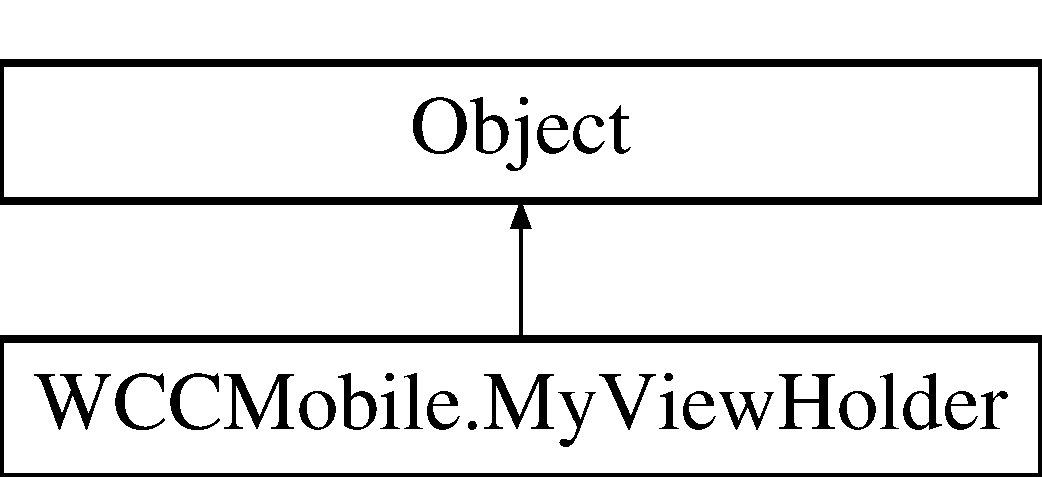
\includegraphics[height=2.000000cm]{class_w_c_c_mobile_1_1_my_view_holder}
\end{center}
\end{figure}
\subsection*{Properties}
\begin{DoxyCompactItemize}
\item 
Text\+View {\bfseries Title}\hspace{0.3cm}{\ttfamily  \mbox{[}get, set\mbox{]}}\hypertarget{class_w_c_c_mobile_1_1_my_view_holder_a91999c3811bee5137a73e95fc3ae6e52}{}\label{class_w_c_c_mobile_1_1_my_view_holder_a91999c3811bee5137a73e95fc3ae6e52}

\end{DoxyCompactItemize}


The documentation for this class was generated from the following file\+:\begin{DoxyCompactItemize}
\item 
Source/\+Activities/Campus\+Map\+Activity.\+cs\end{DoxyCompactItemize}

\hypertarget{class_w_c_c_mobile_1_1_phone_book_activity}{}\section{W\+C\+C\+Mobile.\+Phone\+Book\+Activity Class Reference}
\label{class_w_c_c_mobile_1_1_phone_book_activity}\index{W\+C\+C\+Mobile.\+Phone\+Book\+Activity@{W\+C\+C\+Mobile.\+Phone\+Book\+Activity}}
Inheritance diagram for W\+C\+C\+Mobile.\+Phone\+Book\+Activity\+:\begin{figure}[H]
\begin{center}
\leavevmode
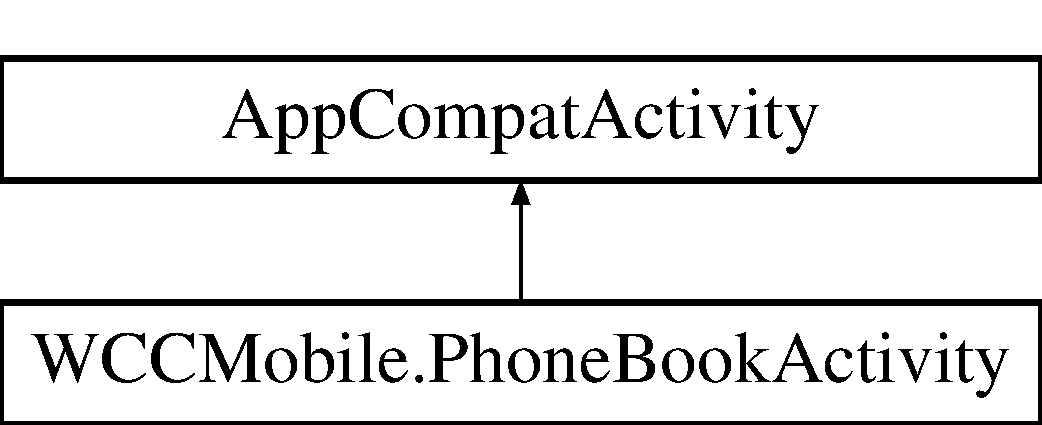
\includegraphics[height=2.000000cm]{class_w_c_c_mobile_1_1_phone_book_activity}
\end{center}
\end{figure}
\subsection*{Public Member Functions}
\begin{DoxyCompactItemize}
\item 
override void \hyperlink{class_w_c_c_mobile_1_1_phone_book_activity_a254e05dc84e87be335afd54b3e8f17ec}{On\+Back\+Pressed} ()
\begin{DoxyCompactList}\small\item\em Called when the activity has detected the user\textquotesingle{}s press of the back key. \end{DoxyCompactList}\end{DoxyCompactItemize}
\subsection*{Static Public Member Functions}
\begin{DoxyCompactItemize}
\item 
static void \hyperlink{class_w_c_c_mobile_1_1_phone_book_activity_a63c39ac58aa08c05cf2cd13e3682ad1f}{Call\+Number} (int Phone\+Key, Activity Caller)
\begin{DoxyCompactList}\small\item\em Function to call numbers from Yellow\+Book.\+txt -\/ Any Activity can call this function provided they pass themselves and the key to the number in the book \end{DoxyCompactList}\item 
static void \hyperlink{class_w_c_c_mobile_1_1_phone_book_activity_a2c0579d4f7de69f1420e3f74dad3ca1f}{Send\+Email} (int Email\+Key, Activity Mailer)
\begin{DoxyCompactList}\small\item\em Method to send emails to address listed in Yellow\+Book.\+txt -\/ Any Activity can call this method provided they pass themselves and the key to the address in the book \end{DoxyCompactList}\item 
static void {\bfseries Alert\+Contact} (int Phone\+Key, Activity Caller)\hypertarget{class_w_c_c_mobile_1_1_phone_book_activity_a1108a3cef14abccc2d96a0b4c05dfe8f}{}\label{class_w_c_c_mobile_1_1_phone_book_activity_a1108a3cef14abccc2d96a0b4c05dfe8f}

\end{DoxyCompactItemize}
\subsection*{Protected Member Functions}
\begin{DoxyCompactItemize}
\item 
override void \hyperlink{class_w_c_c_mobile_1_1_phone_book_activity_a0ce7032ff9764895b2bc66286f24a005}{On\+Create} (Bundle saved\+Instance\+State)
\begin{DoxyCompactList}\small\item\em Called when \mbox{[}create\mbox{]}. \end{DoxyCompactList}\end{DoxyCompactItemize}


\subsection{Member Function Documentation}
\index{W\+C\+C\+Mobile\+::\+Phone\+Book\+Activity@{W\+C\+C\+Mobile\+::\+Phone\+Book\+Activity}!Call\+Number@{Call\+Number}}
\index{Call\+Number@{Call\+Number}!W\+C\+C\+Mobile\+::\+Phone\+Book\+Activity@{W\+C\+C\+Mobile\+::\+Phone\+Book\+Activity}}
\subsubsection[{\texorpdfstring{Call\+Number(int Phone\+Key, Activity Caller)}{CallNumber(int PhoneKey, Activity Caller)}}]{\setlength{\rightskip}{0pt plus 5cm}static void W\+C\+C\+Mobile.\+Phone\+Book\+Activity.\+Call\+Number (
\begin{DoxyParamCaption}
\item[{int}]{Phone\+Key, }
\item[{Activity}]{Caller}
\end{DoxyParamCaption}
)\hspace{0.3cm}{\ttfamily [static]}}\hypertarget{class_w_c_c_mobile_1_1_phone_book_activity_a63c39ac58aa08c05cf2cd13e3682ad1f}{}\label{class_w_c_c_mobile_1_1_phone_book_activity_a63c39ac58aa08c05cf2cd13e3682ad1f}


Function to call numbers from Yellow\+Book.\+txt -\/ Any Activity can call this function provided they pass themselves and the key to the number in the book 


\begin{DoxyParams}{Parameters}
{\em Phone\+Key} & \\
\hline
{\em Caller} & \\
\hline
\end{DoxyParams}
\index{W\+C\+C\+Mobile\+::\+Phone\+Book\+Activity@{W\+C\+C\+Mobile\+::\+Phone\+Book\+Activity}!On\+Back\+Pressed@{On\+Back\+Pressed}}
\index{On\+Back\+Pressed@{On\+Back\+Pressed}!W\+C\+C\+Mobile\+::\+Phone\+Book\+Activity@{W\+C\+C\+Mobile\+::\+Phone\+Book\+Activity}}
\subsubsection[{\texorpdfstring{On\+Back\+Pressed()}{OnBackPressed()}}]{\setlength{\rightskip}{0pt plus 5cm}override void W\+C\+C\+Mobile.\+Phone\+Book\+Activity.\+On\+Back\+Pressed (
\begin{DoxyParamCaption}
{}
\end{DoxyParamCaption}
)}\hypertarget{class_w_c_c_mobile_1_1_phone_book_activity_a254e05dc84e87be335afd54b3e8f17ec}{}\label{class_w_c_c_mobile_1_1_phone_book_activity_a254e05dc84e87be335afd54b3e8f17ec}


Called when the activity has detected the user\textquotesingle{}s press of the back key. 

Called when the activity has detected the user\textquotesingle{}s press of the back key. The default implementation simply finishes the current activity, but you can override this to do whatever you want. 

$<$format type=\char`\"{}text/html\char`\"{}$>$ \href{http://developer.android.com/reference/android/app/Activity.html#onBackPressed()}{\tt \mbox{[}Android Documentation\mbox{]}} $<$/format$>$ 

$<$since version=\char`\"{}\+Added in A\+P\+I level 5\char`\"{}$>$ \index{W\+C\+C\+Mobile\+::\+Phone\+Book\+Activity@{W\+C\+C\+Mobile\+::\+Phone\+Book\+Activity}!On\+Create@{On\+Create}}
\index{On\+Create@{On\+Create}!W\+C\+C\+Mobile\+::\+Phone\+Book\+Activity@{W\+C\+C\+Mobile\+::\+Phone\+Book\+Activity}}
\subsubsection[{\texorpdfstring{On\+Create(\+Bundle saved\+Instance\+State)}{OnCreate(Bundle savedInstanceState)}}]{\setlength{\rightskip}{0pt plus 5cm}override void W\+C\+C\+Mobile.\+Phone\+Book\+Activity.\+On\+Create (
\begin{DoxyParamCaption}
\item[{Bundle}]{saved\+Instance\+State}
\end{DoxyParamCaption}
)\hspace{0.3cm}{\ttfamily [protected]}}\hypertarget{class_w_c_c_mobile_1_1_phone_book_activity_a0ce7032ff9764895b2bc66286f24a005}{}\label{class_w_c_c_mobile_1_1_phone_book_activity_a0ce7032ff9764895b2bc66286f24a005}


Called when \mbox{[}create\mbox{]}. 


\begin{DoxyParams}{Parameters}
{\em saved\+Instance\+State} & State of the saved instance.\\
\hline
\end{DoxyParams}
\index{W\+C\+C\+Mobile\+::\+Phone\+Book\+Activity@{W\+C\+C\+Mobile\+::\+Phone\+Book\+Activity}!Send\+Email@{Send\+Email}}
\index{Send\+Email@{Send\+Email}!W\+C\+C\+Mobile\+::\+Phone\+Book\+Activity@{W\+C\+C\+Mobile\+::\+Phone\+Book\+Activity}}
\subsubsection[{\texorpdfstring{Send\+Email(int Email\+Key, Activity Mailer)}{SendEmail(int EmailKey, Activity Mailer)}}]{\setlength{\rightskip}{0pt plus 5cm}static void W\+C\+C\+Mobile.\+Phone\+Book\+Activity.\+Send\+Email (
\begin{DoxyParamCaption}
\item[{int}]{Email\+Key, }
\item[{Activity}]{Mailer}
\end{DoxyParamCaption}
)\hspace{0.3cm}{\ttfamily [static]}}\hypertarget{class_w_c_c_mobile_1_1_phone_book_activity_a2c0579d4f7de69f1420e3f74dad3ca1f}{}\label{class_w_c_c_mobile_1_1_phone_book_activity_a2c0579d4f7de69f1420e3f74dad3ca1f}


Method to send emails to address listed in Yellow\+Book.\+txt -\/ Any Activity can call this method provided they pass themselves and the key to the address in the book 


\begin{DoxyParams}{Parameters}
{\em Email\+Key} & \\
\hline
{\em Mailer} & \\
\hline
\end{DoxyParams}


The documentation for this class was generated from the following file\+:\begin{DoxyCompactItemize}
\item 
Source/\+Activities/Phone\+Book\+Activity.\+cs\end{DoxyCompactItemize}

\hypertarget{class_w_c_c_mobile_1_1_pin_factory}{}\section{W\+C\+C\+Mobile.\+Pin\+Factory Class Reference}
\label{class_w_c_c_mobile_1_1_pin_factory}\index{W\+C\+C\+Mobile.\+Pin\+Factory@{W\+C\+C\+Mobile.\+Pin\+Factory}}
\subsection*{Public Member Functions}
\begin{DoxyCompactItemize}
\item 
\hyperlink{class_w_c_c_mobile_1_1_pin_factory_a9cdce812f6e1468f5dbcd98aa040ed88}{Pin\+Factory} (Context context)
\begin{DoxyCompactList}\small\item\em Initializes a new instance of the \hyperlink{class_w_c_c_mobile_1_1_pin_factory}{Pin\+Factory} class. \end{DoxyCompactList}\item 
Task$<$ Bitmap $>$ \hyperlink{class_w_c_c_mobile_1_1_pin_factory_aae85d3f9dc2977847b09ffa518c2d310}{Get\+Pin\+Async} (float ratio, int number, int width, int height, float alpha=1)
\begin{DoxyCompactList}\small\item\em Gets the pin asynchronous. \end{DoxyCompactList}\item 
Bitmap \hyperlink{class_w_c_c_mobile_1_1_pin_factory_ac8c67ab242a0a5eec6457a19c2e6e13d}{Get\+Pin} (float ratio, int number, int width, int height, float alpha=1)
\begin{DoxyCompactList}\small\item\em Gets the pin. \end{DoxyCompactList}\item 
Bitmap \hyperlink{class_w_c_c_mobile_1_1_pin_factory_af897a9f6b508c9c8c477fc53f8b511d6}{Get\+Closed\+Pin} (int width, int height)
\begin{DoxyCompactList}\small\item\em Gets the closed pin. \end{DoxyCompactList}\item 
Bitmap \hyperlink{class_w_c_c_mobile_1_1_pin_factory_a071950de5ffa2f0070a3eb8beca79c31}{Get\+Non\+Installed\+Pin} (int width, int height)
\begin{DoxyCompactList}\small\item\em Gets the non installed pin. \end{DoxyCompactList}\end{DoxyCompactItemize}


\subsection{Constructor \& Destructor Documentation}
\index{W\+C\+C\+Mobile\+::\+Pin\+Factory@{W\+C\+C\+Mobile\+::\+Pin\+Factory}!Pin\+Factory@{Pin\+Factory}}
\index{Pin\+Factory@{Pin\+Factory}!W\+C\+C\+Mobile\+::\+Pin\+Factory@{W\+C\+C\+Mobile\+::\+Pin\+Factory}}
\subsubsection[{\texorpdfstring{Pin\+Factory(\+Context context)}{PinFactory(Context context)}}]{\setlength{\rightskip}{0pt plus 5cm}W\+C\+C\+Mobile.\+Pin\+Factory.\+Pin\+Factory (
\begin{DoxyParamCaption}
\item[{Context}]{context}
\end{DoxyParamCaption}
)}\hypertarget{class_w_c_c_mobile_1_1_pin_factory_a9cdce812f6e1468f5dbcd98aa040ed88}{}\label{class_w_c_c_mobile_1_1_pin_factory_a9cdce812f6e1468f5dbcd98aa040ed88}


Initializes a new instance of the \hyperlink{class_w_c_c_mobile_1_1_pin_factory}{Pin\+Factory} class. 


\begin{DoxyParams}{Parameters}
{\em context} & The context.\\
\hline
\end{DoxyParams}


\subsection{Member Function Documentation}
\index{W\+C\+C\+Mobile\+::\+Pin\+Factory@{W\+C\+C\+Mobile\+::\+Pin\+Factory}!Get\+Closed\+Pin@{Get\+Closed\+Pin}}
\index{Get\+Closed\+Pin@{Get\+Closed\+Pin}!W\+C\+C\+Mobile\+::\+Pin\+Factory@{W\+C\+C\+Mobile\+::\+Pin\+Factory}}
\subsubsection[{\texorpdfstring{Get\+Closed\+Pin(int width, int height)}{GetClosedPin(int width, int height)}}]{\setlength{\rightskip}{0pt plus 5cm}Bitmap W\+C\+C\+Mobile.\+Pin\+Factory.\+Get\+Closed\+Pin (
\begin{DoxyParamCaption}
\item[{int}]{width, }
\item[{int}]{height}
\end{DoxyParamCaption}
)}\hypertarget{class_w_c_c_mobile_1_1_pin_factory_af897a9f6b508c9c8c477fc53f8b511d6}{}\label{class_w_c_c_mobile_1_1_pin_factory_af897a9f6b508c9c8c477fc53f8b511d6}


Gets the closed pin. 


\begin{DoxyParams}{Parameters}
{\em width} & The width.\\
\hline
{\em height} & The height.\\
\hline
\end{DoxyParams}
\begin{DoxyReturn}{Returns}

\end{DoxyReturn}
\index{W\+C\+C\+Mobile\+::\+Pin\+Factory@{W\+C\+C\+Mobile\+::\+Pin\+Factory}!Get\+Non\+Installed\+Pin@{Get\+Non\+Installed\+Pin}}
\index{Get\+Non\+Installed\+Pin@{Get\+Non\+Installed\+Pin}!W\+C\+C\+Mobile\+::\+Pin\+Factory@{W\+C\+C\+Mobile\+::\+Pin\+Factory}}
\subsubsection[{\texorpdfstring{Get\+Non\+Installed\+Pin(int width, int height)}{GetNonInstalledPin(int width, int height)}}]{\setlength{\rightskip}{0pt plus 5cm}Bitmap W\+C\+C\+Mobile.\+Pin\+Factory.\+Get\+Non\+Installed\+Pin (
\begin{DoxyParamCaption}
\item[{int}]{width, }
\item[{int}]{height}
\end{DoxyParamCaption}
)}\hypertarget{class_w_c_c_mobile_1_1_pin_factory_a071950de5ffa2f0070a3eb8beca79c31}{}\label{class_w_c_c_mobile_1_1_pin_factory_a071950de5ffa2f0070a3eb8beca79c31}


Gets the non installed pin. 


\begin{DoxyParams}{Parameters}
{\em width} & The width.\\
\hline
{\em height} & The height.\\
\hline
\end{DoxyParams}
\begin{DoxyReturn}{Returns}

\end{DoxyReturn}
\index{W\+C\+C\+Mobile\+::\+Pin\+Factory@{W\+C\+C\+Mobile\+::\+Pin\+Factory}!Get\+Pin@{Get\+Pin}}
\index{Get\+Pin@{Get\+Pin}!W\+C\+C\+Mobile\+::\+Pin\+Factory@{W\+C\+C\+Mobile\+::\+Pin\+Factory}}
\subsubsection[{\texorpdfstring{Get\+Pin(float ratio, int number, int width, int height, float alpha=1)}{GetPin(float ratio, int number, int width, int height, float alpha=1)}}]{\setlength{\rightskip}{0pt plus 5cm}Bitmap W\+C\+C\+Mobile.\+Pin\+Factory.\+Get\+Pin (
\begin{DoxyParamCaption}
\item[{float}]{ratio, }
\item[{int}]{number, }
\item[{int}]{width, }
\item[{int}]{height, }
\item[{float}]{alpha = {\ttfamily 1}}
\end{DoxyParamCaption}
)}\hypertarget{class_w_c_c_mobile_1_1_pin_factory_ac8c67ab242a0a5eec6457a19c2e6e13d}{}\label{class_w_c_c_mobile_1_1_pin_factory_ac8c67ab242a0a5eec6457a19c2e6e13d}


Gets the pin. 


\begin{DoxyParams}{Parameters}
{\em ratio} & The ratio.\\
\hline
{\em number} & The number.\\
\hline
{\em width} & The width.\\
\hline
{\em height} & The height.\\
\hline
{\em alpha} & The alpha.\\
\hline
\end{DoxyParams}
\begin{DoxyReturn}{Returns}

\end{DoxyReturn}
\index{W\+C\+C\+Mobile\+::\+Pin\+Factory@{W\+C\+C\+Mobile\+::\+Pin\+Factory}!Get\+Pin\+Async@{Get\+Pin\+Async}}
\index{Get\+Pin\+Async@{Get\+Pin\+Async}!W\+C\+C\+Mobile\+::\+Pin\+Factory@{W\+C\+C\+Mobile\+::\+Pin\+Factory}}
\subsubsection[{\texorpdfstring{Get\+Pin\+Async(float ratio, int number, int width, int height, float alpha=1)}{GetPinAsync(float ratio, int number, int width, int height, float alpha=1)}}]{\setlength{\rightskip}{0pt plus 5cm}Task$<$Bitmap$>$ W\+C\+C\+Mobile.\+Pin\+Factory.\+Get\+Pin\+Async (
\begin{DoxyParamCaption}
\item[{float}]{ratio, }
\item[{int}]{number, }
\item[{int}]{width, }
\item[{int}]{height, }
\item[{float}]{alpha = {\ttfamily 1}}
\end{DoxyParamCaption}
)}\hypertarget{class_w_c_c_mobile_1_1_pin_factory_aae85d3f9dc2977847b09ffa518c2d310}{}\label{class_w_c_c_mobile_1_1_pin_factory_aae85d3f9dc2977847b09ffa518c2d310}


Gets the pin asynchronous. 


\begin{DoxyParams}{Parameters}
{\em ratio} & The ratio.\\
\hline
{\em number} & The number.\\
\hline
{\em width} & The width.\\
\hline
{\em height} & The height.\\
\hline
{\em alpha} & The alpha.\\
\hline
\end{DoxyParams}
\begin{DoxyReturn}{Returns}

\end{DoxyReturn}


The documentation for this class was generated from the following file\+:\begin{DoxyCompactItemize}
\item 
Source/\+Controls/Pin\+Factory.\+cs\end{DoxyCompactItemize}

\hypertarget{class_w_c_c_mobile_1_1_schedule_fragment}{}\section{W\+C\+C\+Mobile.\+Schedule\+Fragment Class Reference}
\label{class_w_c_c_mobile_1_1_schedule_fragment}\index{W\+C\+C\+Mobile.\+Schedule\+Fragment@{W\+C\+C\+Mobile.\+Schedule\+Fragment}}
Inheritance diagram for W\+C\+C\+Mobile.\+Schedule\+Fragment\+:\begin{figure}[H]
\begin{center}
\leavevmode
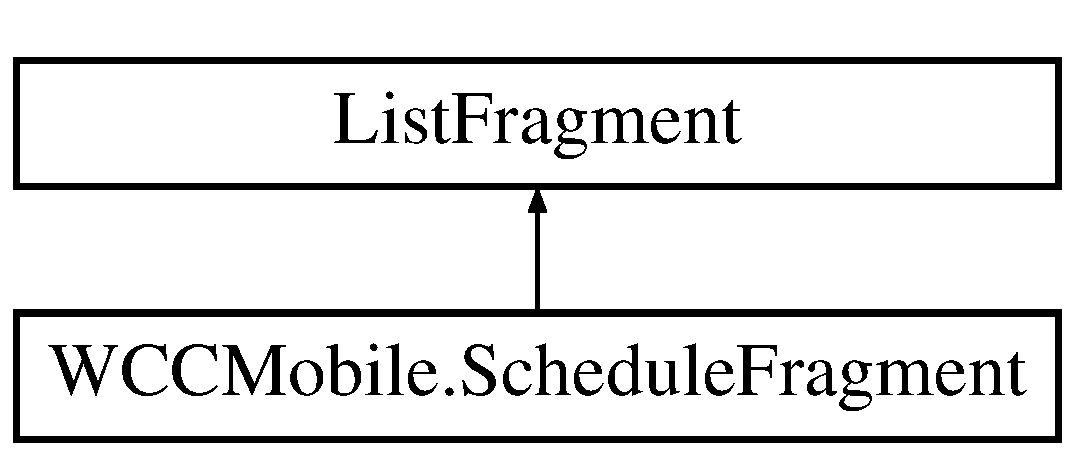
\includegraphics[height=2.000000cm]{class_w_c_c_mobile_1_1_schedule_fragment}
\end{center}
\end{figure}


The documentation for this class was generated from the following file\+:\begin{DoxyCompactItemize}
\item 
Source/\+Fragments/Schedule\+Fragment.\+cs\end{DoxyCompactItemize}

\hypertarget{class_w_c_c_mobile_1_1_schedule_history}{}\section{W\+C\+C\+Mobile.\+Schedule\+History Class Reference}
\label{class_w_c_c_mobile_1_1_schedule_history}\index{W\+C\+C\+Mobile.\+Schedule\+History@{W\+C\+C\+Mobile.\+Schedule\+History}}


The documentation for this class was generated from the following file\+:\begin{DoxyCompactItemize}
\item 
Source/\+Helpers/Schedule\+History.\+cs\end{DoxyCompactItemize}

\hypertarget{class_w_c_c_mobile_1_1_models_1_1_schedule_item}{}\section{W\+C\+C\+Mobile.\+Models.\+Schedule\+Item Class Reference}
\label{class_w_c_c_mobile_1_1_models_1_1_schedule_item}\index{W\+C\+C\+Mobile.\+Models.\+Schedule\+Item@{W\+C\+C\+Mobile.\+Models.\+Schedule\+Item}}
\subsection*{Public Member Functions}
\begin{DoxyCompactItemize}
\item 
override bool {\bfseries Equals} (object obj)\hypertarget{class_w_c_c_mobile_1_1_models_1_1_schedule_item_a5175c56d2815231179968c78c250e4d2}{}\label{class_w_c_c_mobile_1_1_models_1_1_schedule_item_a5175c56d2815231179968c78c250e4d2}

\item 
bool {\bfseries Equals} (\hyperlink{class_w_c_c_mobile_1_1_models_1_1_schedule_item}{Schedule\+Item} other)\hypertarget{class_w_c_c_mobile_1_1_models_1_1_schedule_item_adb957c9403cd42982874c4840eb28f8c}{}\label{class_w_c_c_mobile_1_1_models_1_1_schedule_item_adb957c9403cd42982874c4840eb28f8c}

\item 
override int {\bfseries Get\+Hash\+Code} ()\hypertarget{class_w_c_c_mobile_1_1_models_1_1_schedule_item_af118b43db33df259e0c9377fcc98a1ac}{}\label{class_w_c_c_mobile_1_1_models_1_1_schedule_item_af118b43db33df259e0c9377fcc98a1ac}

\end{DoxyCompactItemize}
\subsection*{Properties}
\begin{DoxyCompactItemize}
\item 
int {\bfseries Id}\hspace{0.3cm}{\ttfamily  \mbox{[}get, set\mbox{]}}\hypertarget{class_w_c_c_mobile_1_1_models_1_1_schedule_item_a42afe45613fdae1485c372622b95ccea}{}\label{class_w_c_c_mobile_1_1_models_1_1_schedule_item_a42afe45613fdae1485c372622b95ccea}

\item 
string {\bfseries Street}\hspace{0.3cm}{\ttfamily  \mbox{[}get, set\mbox{]}}\hypertarget{class_w_c_c_mobile_1_1_models_1_1_schedule_item_a06ac931092ff9cbc150934105b66ea5a}{}\label{class_w_c_c_mobile_1_1_models_1_1_schedule_item_a06ac931092ff9cbc150934105b66ea5a}

\item 
string {\bfseries Name}\hspace{0.3cm}{\ttfamily  \mbox{[}get, set\mbox{]}}\hypertarget{class_w_c_c_mobile_1_1_models_1_1_schedule_item_a6caf66949e0c699837a1723ba4adfd3e}{}\label{class_w_c_c_mobile_1_1_models_1_1_schedule_item_a6caf66949e0c699837a1723ba4adfd3e}

\item 
int {\bfseries Station\+Type}\hspace{0.3cm}{\ttfamily  \mbox{[}get, set\mbox{]}}\hypertarget{class_w_c_c_mobile_1_1_models_1_1_schedule_item_a7af165503d2d9d85cd5662f1d8ee3785}{}\label{class_w_c_c_mobile_1_1_models_1_1_schedule_item_a7af165503d2d9d85cd5662f1d8ee3785}

\item 
bool {\bfseries b}\hspace{0.3cm}{\ttfamily  \mbox{[}get, set\mbox{]}}\hypertarget{class_w_c_c_mobile_1_1_models_1_1_schedule_item_ab8cf60bd452c817c7cad092f6d53b162}{}\label{class_w_c_c_mobile_1_1_models_1_1_schedule_item_ab8cf60bd452c817c7cad092f6d53b162}

\item 
bool {\bfseries su}\hspace{0.3cm}{\ttfamily  \mbox{[}get, set\mbox{]}}\hypertarget{class_w_c_c_mobile_1_1_models_1_1_schedule_item_a8eaf7b67c6d99c80127a41c27bddd4a6}{}\label{class_w_c_c_mobile_1_1_models_1_1_schedule_item_a8eaf7b67c6d99c80127a41c27bddd4a6}

\item 
bool {\bfseries t}\hspace{0.3cm}{\ttfamily  \mbox{[}get, set\mbox{]}}\hypertarget{class_w_c_c_mobile_1_1_models_1_1_schedule_item_ad1ade83c77908a45bfd6a8ec54561a55}{}\label{class_w_c_c_mobile_1_1_models_1_1_schedule_item_ad1ade83c77908a45bfd6a8ec54561a55}

\item 
bool {\bfseries bk}\hspace{0.3cm}{\ttfamily  \mbox{[}get, set\mbox{]}}\hypertarget{class_w_c_c_mobile_1_1_models_1_1_schedule_item_a98cabd9e67963ab06eca60229b785177}{}\label{class_w_c_c_mobile_1_1_models_1_1_schedule_item_a98cabd9e67963ab06eca60229b785177}

\item 
bool {\bfseries bl}\hspace{0.3cm}{\ttfamily  \mbox{[}get, set\mbox{]}}\hypertarget{class_w_c_c_mobile_1_1_models_1_1_schedule_item_acd488ca0710bbbee958b3e62a2fd0932}{}\label{class_w_c_c_mobile_1_1_models_1_1_schedule_item_acd488ca0710bbbee958b3e62a2fd0932}

\item 
double {\bfseries Latitude}\hspace{0.3cm}{\ttfamily  \mbox{[}get, set\mbox{]}}\hypertarget{class_w_c_c_mobile_1_1_models_1_1_schedule_item_ae3b442e108a1905dfeaba6c1127350df}{}\label{class_w_c_c_mobile_1_1_models_1_1_schedule_item_ae3b442e108a1905dfeaba6c1127350df}

\item 
double {\bfseries Longitude}\hspace{0.3cm}{\ttfamily  \mbox{[}get, set\mbox{]}}\hypertarget{class_w_c_c_mobile_1_1_models_1_1_schedule_item_a60466ef3c7863351ce9816fa0843727e}{}\label{class_w_c_c_mobile_1_1_models_1_1_schedule_item_a60466ef3c7863351ce9816fa0843727e}

\item 
int {\bfseries Empty\+Slot\+Count}\hspace{0.3cm}{\ttfamily  \mbox{[}get, set\mbox{]}}\hypertarget{class_w_c_c_mobile_1_1_models_1_1_schedule_item_a850291dafbc6d17023eb79e1ea065192}{}\label{class_w_c_c_mobile_1_1_models_1_1_schedule_item_a850291dafbc6d17023eb79e1ea065192}

\item 
int {\bfseries dx}\hspace{0.3cm}{\ttfamily  \mbox{[}get, set\mbox{]}}\hypertarget{class_w_c_c_mobile_1_1_models_1_1_schedule_item_a322a0357de9938bd6c2ae06976946a68}{}\label{class_w_c_c_mobile_1_1_models_1_1_schedule_item_a322a0357de9938bd6c2ae06976946a68}

\item 
int {\bfseries Bike\+Count}\hspace{0.3cm}{\ttfamily  \mbox{[}get, set\mbox{]}}\hypertarget{class_w_c_c_mobile_1_1_models_1_1_schedule_item_a39af18a7bd4a52b30c42ef196e171342}{}\label{class_w_c_c_mobile_1_1_models_1_1_schedule_item_a39af18a7bd4a52b30c42ef196e171342}

\item 
int {\bfseries bx}\hspace{0.3cm}{\ttfamily  \mbox{[}get, set\mbox{]}}\hypertarget{class_w_c_c_mobile_1_1_models_1_1_schedule_item_acd53e3ae65c390b85f709c78ea839214}{}\label{class_w_c_c_mobile_1_1_models_1_1_schedule_item_acd53e3ae65c390b85f709c78ea839214}

\item 
\hyperlink{struct_w_c_c_mobile_1_1_location}{Location} {\bfseries Location}\hspace{0.3cm}{\ttfamily  \mbox{[}get\mbox{]}}\hypertarget{class_w_c_c_mobile_1_1_models_1_1_schedule_item_a994ac1beccddc5b04eda73b8f0a33bc2}{}\label{class_w_c_c_mobile_1_1_models_1_1_schedule_item_a994ac1beccddc5b04eda73b8f0a33bc2}

\item 
int {\bfseries Capacity}\hspace{0.3cm}{\ttfamily  \mbox{[}get\mbox{]}}\hypertarget{class_w_c_c_mobile_1_1_models_1_1_schedule_item_adcb68af24eeae563aa5e98f2a9094632}{}\label{class_w_c_c_mobile_1_1_models_1_1_schedule_item_adcb68af24eeae563aa5e98f2a9094632}

\item 
bool {\bfseries Installed}\hspace{0.3cm}{\ttfamily  \mbox{[}get\mbox{]}}\hypertarget{class_w_c_c_mobile_1_1_models_1_1_schedule_item_a4ba3ad838bb019296ce6a8cc90ff527a}{}\label{class_w_c_c_mobile_1_1_models_1_1_schedule_item_a4ba3ad838bb019296ce6a8cc90ff527a}

\item 
bool {\bfseries Temporary}\hspace{0.3cm}{\ttfamily  \mbox{[}get\mbox{]}}\hypertarget{class_w_c_c_mobile_1_1_models_1_1_schedule_item_a899b7cd610777f8e88cbef5f13dcf417}{}\label{class_w_c_c_mobile_1_1_models_1_1_schedule_item_a899b7cd610777f8e88cbef5f13dcf417}

\item 
bool {\bfseries Locked}\hspace{0.3cm}{\ttfamily  \mbox{[}get\mbox{]}}\hypertarget{class_w_c_c_mobile_1_1_models_1_1_schedule_item_a59b60f211a37137748beaba437da7afe}{}\label{class_w_c_c_mobile_1_1_models_1_1_schedule_item_a59b60f211a37137748beaba437da7afe}

\item 
string {\bfseries Location\+Url}\hspace{0.3cm}{\ttfamily  \mbox{[}get\mbox{]}}\hypertarget{class_w_c_c_mobile_1_1_models_1_1_schedule_item_abcc77ea16b0e0d25262d94772096b9f2}{}\label{class_w_c_c_mobile_1_1_models_1_1_schedule_item_abcc77ea16b0e0d25262d94772096b9f2}

\end{DoxyCompactItemize}


The documentation for this class was generated from the following file\+:\begin{DoxyCompactItemize}
\item 
Source/\+Models/Schedule\+Item.\+cs\end{DoxyCompactItemize}

\hypertarget{class_w_c_c_mobile_1_1_schedule_manager}{}\section{W\+C\+C\+Mobile.\+Schedule\+Manager Class Reference}
\label{class_w_c_c_mobile_1_1_schedule_manager}\index{W\+C\+C\+Mobile.\+Schedule\+Manager@{W\+C\+C\+Mobile.\+Schedule\+Manager}}
\subsection*{Public Member Functions}
\begin{DoxyCompactItemize}
\item 
{\bfseries Schedule\+Manager} (Context context)\hypertarget{class_w_c_c_mobile_1_1_schedule_manager_a9dbc4604f85762b82dfc0c2a61adbf63}{}\label{class_w_c_c_mobile_1_1_schedule_manager_a9dbc4604f85762b82dfc0c2a61adbf63}

\item 
Hash\+Set$<$ int $>$ {\bfseries Get\+Schedule\+Item\+Ids} ()\hypertarget{class_w_c_c_mobile_1_1_schedule_manager_a6885a2183fceb0e1081929192781de20}{}\label{class_w_c_c_mobile_1_1_schedule_manager_a6885a2183fceb0e1081929192781de20}

\end{DoxyCompactItemize}
\subsection*{Static Public Member Functions}
\begin{DoxyCompactItemize}
\item 
static \hyperlink{class_w_c_c_mobile_1_1_schedule_manager}{Schedule\+Manager} {\bfseries Obtain} (Context context)\hypertarget{class_w_c_c_mobile_1_1_schedule_manager_addd61b930a1af249a754fab52abe0d38}{}\label{class_w_c_c_mobile_1_1_schedule_manager_addd61b930a1af249a754fab52abe0d38}

\end{DoxyCompactItemize}
\subsection*{Properties}
\begin{DoxyCompactItemize}
\item 
object {\bfseries Last\+Schedule}\hspace{0.3cm}{\ttfamily  \mbox{[}get, set\mbox{]}}\hypertarget{class_w_c_c_mobile_1_1_schedule_manager_a409ab82e52432f798e97963b23fbc98c}{}\label{class_w_c_c_mobile_1_1_schedule_manager_a409ab82e52432f798e97963b23fbc98c}

\end{DoxyCompactItemize}
\subsection*{Events}
\begin{DoxyCompactItemize}
\item 
static Event\+Handler {\bfseries Favorites\+Changed}\hypertarget{class_w_c_c_mobile_1_1_schedule_manager_ae50ee038373a79b31fccc2885901d39f}{}\label{class_w_c_c_mobile_1_1_schedule_manager_ae50ee038373a79b31fccc2885901d39f}

\end{DoxyCompactItemize}


The documentation for this class was generated from the following file\+:\begin{DoxyCompactItemize}
\item 
Source/\+Adapters/Schedule\+Manager.\+cs\end{DoxyCompactItemize}

\hypertarget{class_w_c_c_mobile_1_1_schedule_observer}{}\section{W\+C\+C\+Mobile.\+Schedule\+Observer Class Reference}
\label{class_w_c_c_mobile_1_1_schedule_observer}\index{W\+C\+C\+Mobile.\+Schedule\+Observer@{W\+C\+C\+Mobile.\+Schedule\+Observer}}
Inheritance diagram for W\+C\+C\+Mobile.\+Schedule\+Observer\+:\begin{figure}[H]
\begin{center}
\leavevmode
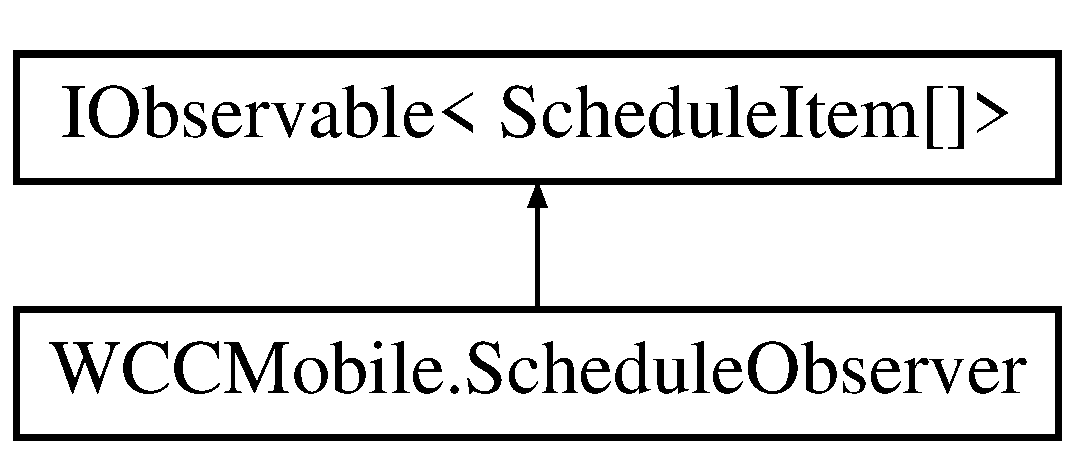
\includegraphics[height=2.000000cm]{class_w_c_c_mobile_1_1_schedule_observer}
\end{center}
\end{figure}
\subsection*{Public Member Functions}
\begin{DoxyCompactItemize}
\item 
{\bfseries Schedule\+Observer} (Time\+Span freshness\+Timeout)\hypertarget{class_w_c_c_mobile_1_1_schedule_observer_aa2671067f6f4e653c53bbd18d30ef138}{}\label{class_w_c_c_mobile_1_1_schedule_observer_aa2671067f6f4e653c53bbd18d30ef138}

\item 
async Task$<$ \hyperlink{class_w_c_c_mobile_1_1_models_1_1_schedule_item}{Schedule\+Item}\mbox{[}$\,$\mbox{]}$>$ {\bfseries Get\+Stations} (bool force\+Refresh=false, Action$<$ string $>$ data\+Cacher=null)\hypertarget{class_w_c_c_mobile_1_1_schedule_observer_a188eb1decb6645152cc60c818b660109}{}\label{class_w_c_c_mobile_1_1_schedule_observer_a188eb1decb6645152cc60c818b660109}

\item 
I\+Disposable {\bfseries Subscribe} (I\+Observer$<$ \hyperlink{class_w_c_c_mobile_1_1_models_1_1_schedule_item}{Schedule\+Item}\mbox{[}$\,$\mbox{]}$>$ observer)\hypertarget{class_w_c_c_mobile_1_1_schedule_observer_a65071c6f65680de277f70531e2719d25}{}\label{class_w_c_c_mobile_1_1_schedule_observer_a65071c6f65680de277f70531e2719d25}

\end{DoxyCompactItemize}
\subsection*{Static Public Member Functions}
\begin{DoxyCompactItemize}
\item 
static \hyperlink{class_w_c_c_mobile_1_1_models_1_1_schedule_item}{Schedule\+Item}\mbox{[}$\,$\mbox{]} {\bfseries Get\+Stations\+Around} (\hyperlink{class_w_c_c_mobile_1_1_models_1_1_schedule_item}{Schedule\+Item}\mbox{[}$\,$\mbox{]} stations, \hyperlink{struct_w_c_c_mobile_1_1_location}{Location} location, double min\+Distance=100, int max\+Items=4)\hypertarget{class_w_c_c_mobile_1_1_schedule_observer_a36bc0a2987055ca966664ada81e5088c}{}\label{class_w_c_c_mobile_1_1_schedule_observer_a36bc0a2987055ca966664ada81e5088c}

\end{DoxyCompactItemize}
\subsection*{Static Public Attributes}
\begin{DoxyCompactItemize}
\item 
static readonly Func$<$ \hyperlink{class_w_c_c_mobile_1_1_models_1_1_schedule_item}{Schedule\+Item}, bool $>$ {\bfseries Available\+Bike\+Station\+Predicate} = s =$>$ s.\+Bike\+Count $>$ 1 \&\& s.\+Empty\+Slot\+Count $>$ 1\hypertarget{class_w_c_c_mobile_1_1_schedule_observer_a718156c9e114254fbcdf9ce3d7fcbad7}{}\label{class_w_c_c_mobile_1_1_schedule_observer_a718156c9e114254fbcdf9ce3d7fcbad7}

\item 
static readonly \hyperlink{class_w_c_c_mobile_1_1_schedule_observer}{Schedule\+Observer} {\bfseries Instance} = new \hyperlink{class_w_c_c_mobile_1_1_schedule_observer}{Schedule\+Observer}()\hypertarget{class_w_c_c_mobile_1_1_schedule_observer_a8e5563a0a73e96a376a84767c5e05849}{}\label{class_w_c_c_mobile_1_1_schedule_observer_a8e5563a0a73e96a376a84767c5e05849}

\end{DoxyCompactItemize}
\subsection*{Properties}
\begin{DoxyCompactItemize}
\item 
Date\+Time {\bfseries Last\+Update\+Time}\hspace{0.3cm}{\ttfamily  \mbox{[}get\mbox{]}}\hypertarget{class_w_c_c_mobile_1_1_schedule_observer_a1e670ceb3c93e76eabf3b9603f9e3136}{}\label{class_w_c_c_mobile_1_1_schedule_observer_a1e670ceb3c93e76eabf3b9603f9e3136}

\item 
\hyperlink{class_w_c_c_mobile_1_1_models_1_1_schedule_item}{Schedule\+Item}\mbox{[}$\,$\mbox{]} {\bfseries Last\+Schedule\+Items}\hspace{0.3cm}{\ttfamily  \mbox{[}get\mbox{]}}\hypertarget{class_w_c_c_mobile_1_1_schedule_observer_a0ea021f1a7c4e0d4dd0dd0f6c9364500}{}\label{class_w_c_c_mobile_1_1_schedule_observer_a0ea021f1a7c4e0d4dd0dd0f6c9364500}

\item 
bool {\bfseries Has\+Cached\+Data}\hspace{0.3cm}{\ttfamily  \mbox{[}get\mbox{]}}\hypertarget{class_w_c_c_mobile_1_1_schedule_observer_a9e4207b94e505bb9b8fb83661942d9cd}{}\label{class_w_c_c_mobile_1_1_schedule_observer_a9e4207b94e505bb9b8fb83661942d9cd}

\item 
object {\bfseries Last\+Schedule\+Item}\hspace{0.3cm}{\ttfamily  \mbox{[}get, set\mbox{]}}\hypertarget{class_w_c_c_mobile_1_1_schedule_observer_a99d10a1c554bc9c71532795d62b4c3f0}{}\label{class_w_c_c_mobile_1_1_schedule_observer_a99d10a1c554bc9c71532795d62b4c3f0}

\end{DoxyCompactItemize}


The documentation for this class was generated from the following file\+:\begin{DoxyCompactItemize}
\item 
Source/\+Helpers/Schedule\+Observer.\+cs\end{DoxyCompactItemize}

\hypertarget{class_w_c_c_mobile_1_1_schedule_root_object}{}\section{W\+C\+C\+Mobile.\+Schedule\+Root\+Object Class Reference}
\label{class_w_c_c_mobile_1_1_schedule_root_object}\index{W\+C\+C\+Mobile.\+Schedule\+Root\+Object@{W\+C\+C\+Mobile.\+Schedule\+Root\+Object}}
\subsection*{Properties}
\begin{DoxyCompactItemize}
\item 
long {\bfseries Timestamp}\hspace{0.3cm}{\ttfamily  \mbox{[}get, set\mbox{]}}\hypertarget{class_w_c_c_mobile_1_1_schedule_root_object_a47a015576c0adf06f2274ff294b1319b}{}\label{class_w_c_c_mobile_1_1_schedule_root_object_a47a015576c0adf06f2274ff294b1319b}

\item 
bool {\bfseries Scheme\+Suspended}\hspace{0.3cm}{\ttfamily  \mbox{[}get, set\mbox{]}}\hypertarget{class_w_c_c_mobile_1_1_schedule_root_object_a99115104f9ae84b517c43bfc7ffd053d}{}\label{class_w_c_c_mobile_1_1_schedule_root_object_a99115104f9ae84b517c43bfc7ffd053d}

\item 
List$<$ \hyperlink{class_w_c_c_mobile_1_1_models_1_1_schedule_item}{Schedule\+Item} $>$ {\bfseries Schedule}\hspace{0.3cm}{\ttfamily  \mbox{[}get, set\mbox{]}}\hypertarget{class_w_c_c_mobile_1_1_schedule_root_object_a5e12dc3ab3b5c1160726b69f66847929}{}\label{class_w_c_c_mobile_1_1_schedule_root_object_a5e12dc3ab3b5c1160726b69f66847929}

\end{DoxyCompactItemize}


The documentation for this class was generated from the following file\+:\begin{DoxyCompactItemize}
\item 
Source/\+Models/Schedule\+Root\+Object.\+cs\end{DoxyCompactItemize}

\hypertarget{class_w_c_c_mobile_1_1_switchable_fab}{}\section{W\+C\+C\+Mobile.\+Switchable\+Fab Class Reference}
\label{class_w_c_c_mobile_1_1_switchable_fab}\index{W\+C\+C\+Mobile.\+Switchable\+Fab@{W\+C\+C\+Mobile.\+Switchable\+Fab}}
Inheritance diagram for W\+C\+C\+Mobile.\+Switchable\+Fab\+:\begin{figure}[H]
\begin{center}
\leavevmode
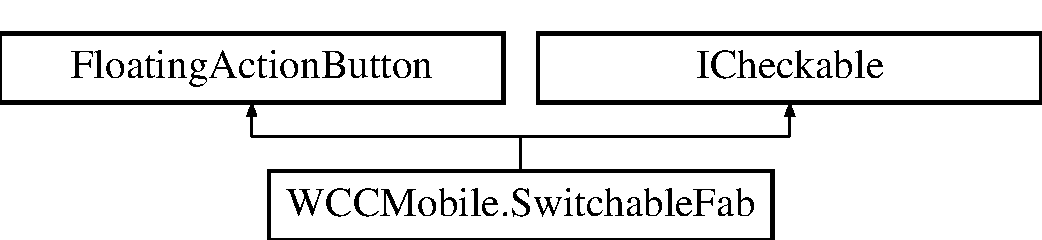
\includegraphics[height=2.000000cm]{class_w_c_c_mobile_1_1_switchable_fab}
\end{center}
\end{figure}
\subsection*{Public Member Functions}
\begin{DoxyCompactItemize}
\item 
\hyperlink{class_w_c_c_mobile_1_1_switchable_fab_a8427440d9a6834d9a8f4debaf905da7b}{Switchable\+Fab} (Context context)
\begin{DoxyCompactList}\small\item\em Initializes a new instance of the \hyperlink{class_w_c_c_mobile_1_1_switchable_fab}{Switchable\+Fab} class. \end{DoxyCompactList}\item 
\hyperlink{class_w_c_c_mobile_1_1_switchable_fab_a9674454567b1e5661bca32b57ba10ab2}{Switchable\+Fab} (Context context, I\+Attribute\+Set attrs)
\begin{DoxyCompactList}\small\item\em Initializes a new instance of the \hyperlink{class_w_c_c_mobile_1_1_switchable_fab}{Switchable\+Fab} class. \end{DoxyCompactList}\item 
\hyperlink{class_w_c_c_mobile_1_1_switchable_fab_ab4d24c06b64058307cbaeae023a2e142}{Switchable\+Fab} (Context context, I\+Attribute\+Set attrs, int def\+Style)
\begin{DoxyCompactList}\small\item\em Initializes a new instance of the \hyperlink{class_w_c_c_mobile_1_1_switchable_fab}{Switchable\+Fab} class. \end{DoxyCompactList}\item 
\hyperlink{class_w_c_c_mobile_1_1_switchable_fab_a253c5a3888796e89248ff53a9772b2e2}{Switchable\+Fab} (Int\+Ptr handle, Jni\+Handle\+Ownership own)
\begin{DoxyCompactList}\small\item\em Initializes a new instance of the \hyperlink{class_w_c_c_mobile_1_1_switchable_fab}{Switchable\+Fab} class. \end{DoxyCompactList}\item 
override bool \hyperlink{class_w_c_c_mobile_1_1_switchable_fab_a51259df9d79a50bacc6493c950430e6a}{Perform\+Click} ()
\begin{DoxyCompactList}\small\item\em Call this view\textquotesingle{}s On\+Click\+Listener, if it is defined. \end{DoxyCompactList}\item 
void \hyperlink{class_w_c_c_mobile_1_1_switchable_fab_a39abe74f848ac20dc4afa71b3d9b3a7f}{Toggle} ()
\begin{DoxyCompactList}\small\item\em Change the checked state of the view to the inverse of its current state \end{DoxyCompactList}\item 
override int\mbox{[}$\,$\mbox{]} \hyperlink{class_w_c_c_mobile_1_1_switchable_fab_ac48bee3d795175bebe091916c459bf20}{On\+Create\+Drawable\+State} (int extra\+Space)
\begin{DoxyCompactList}\small\item\em Generate the new {\ttfamily T\+:\+Android.\+Graphics.\+Drawables.\+Drawable} state for this view. \end{DoxyCompactList}\item 
void \hyperlink{class_w_c_c_mobile_1_1_switchable_fab_aca7b2f599c6591440ac4edcd6201f542}{Switch} ()
\begin{DoxyCompactList}\small\item\em Switches this instance. \end{DoxyCompactList}\end{DoxyCompactItemize}
\subsection*{Properties}
\begin{DoxyCompactItemize}
\item 
bool \hyperlink{class_w_c_c_mobile_1_1_switchable_fab_a5e47f1f153ff63519425d35f0d4515d7}{Checked}\hspace{0.3cm}{\ttfamily  \mbox{[}get, set\mbox{]}}
\end{DoxyCompactItemize}


\subsection{Constructor \& Destructor Documentation}
\index{W\+C\+C\+Mobile\+::\+Switchable\+Fab@{W\+C\+C\+Mobile\+::\+Switchable\+Fab}!Switchable\+Fab@{Switchable\+Fab}}
\index{Switchable\+Fab@{Switchable\+Fab}!W\+C\+C\+Mobile\+::\+Switchable\+Fab@{W\+C\+C\+Mobile\+::\+Switchable\+Fab}}
\subsubsection[{\texorpdfstring{Switchable\+Fab(\+Context context)}{SwitchableFab(Context context)}}]{\setlength{\rightskip}{0pt plus 5cm}W\+C\+C\+Mobile.\+Switchable\+Fab.\+Switchable\+Fab (
\begin{DoxyParamCaption}
\item[{Context}]{context}
\end{DoxyParamCaption}
)}\hypertarget{class_w_c_c_mobile_1_1_switchable_fab_a8427440d9a6834d9a8f4debaf905da7b}{}\label{class_w_c_c_mobile_1_1_switchable_fab_a8427440d9a6834d9a8f4debaf905da7b}


Initializes a new instance of the \hyperlink{class_w_c_c_mobile_1_1_switchable_fab}{Switchable\+Fab} class. 


\begin{DoxyParams}{Parameters}
{\em context} & The context.\\
\hline
\end{DoxyParams}
\index{W\+C\+C\+Mobile\+::\+Switchable\+Fab@{W\+C\+C\+Mobile\+::\+Switchable\+Fab}!Switchable\+Fab@{Switchable\+Fab}}
\index{Switchable\+Fab@{Switchable\+Fab}!W\+C\+C\+Mobile\+::\+Switchable\+Fab@{W\+C\+C\+Mobile\+::\+Switchable\+Fab}}
\subsubsection[{\texorpdfstring{Switchable\+Fab(\+Context context, I\+Attribute\+Set attrs)}{SwitchableFab(Context context, IAttributeSet attrs)}}]{\setlength{\rightskip}{0pt plus 5cm}W\+C\+C\+Mobile.\+Switchable\+Fab.\+Switchable\+Fab (
\begin{DoxyParamCaption}
\item[{Context}]{context, }
\item[{I\+Attribute\+Set}]{attrs}
\end{DoxyParamCaption}
)}\hypertarget{class_w_c_c_mobile_1_1_switchable_fab_a9674454567b1e5661bca32b57ba10ab2}{}\label{class_w_c_c_mobile_1_1_switchable_fab_a9674454567b1e5661bca32b57ba10ab2}


Initializes a new instance of the \hyperlink{class_w_c_c_mobile_1_1_switchable_fab}{Switchable\+Fab} class. 


\begin{DoxyParams}{Parameters}
{\em context} & The context.\\
\hline
{\em attrs} & The attrs.\\
\hline
\end{DoxyParams}
\index{W\+C\+C\+Mobile\+::\+Switchable\+Fab@{W\+C\+C\+Mobile\+::\+Switchable\+Fab}!Switchable\+Fab@{Switchable\+Fab}}
\index{Switchable\+Fab@{Switchable\+Fab}!W\+C\+C\+Mobile\+::\+Switchable\+Fab@{W\+C\+C\+Mobile\+::\+Switchable\+Fab}}
\subsubsection[{\texorpdfstring{Switchable\+Fab(\+Context context, I\+Attribute\+Set attrs, int def\+Style)}{SwitchableFab(Context context, IAttributeSet attrs, int defStyle)}}]{\setlength{\rightskip}{0pt plus 5cm}W\+C\+C\+Mobile.\+Switchable\+Fab.\+Switchable\+Fab (
\begin{DoxyParamCaption}
\item[{Context}]{context, }
\item[{I\+Attribute\+Set}]{attrs, }
\item[{int}]{def\+Style}
\end{DoxyParamCaption}
)}\hypertarget{class_w_c_c_mobile_1_1_switchable_fab_ab4d24c06b64058307cbaeae023a2e142}{}\label{class_w_c_c_mobile_1_1_switchable_fab_ab4d24c06b64058307cbaeae023a2e142}


Initializes a new instance of the \hyperlink{class_w_c_c_mobile_1_1_switchable_fab}{Switchable\+Fab} class. 


\begin{DoxyParams}{Parameters}
{\em context} & The context.\\
\hline
{\em attrs} & The attrs.\\
\hline
{\em def\+Style} & The definition style.\\
\hline
\end{DoxyParams}
\index{W\+C\+C\+Mobile\+::\+Switchable\+Fab@{W\+C\+C\+Mobile\+::\+Switchable\+Fab}!Switchable\+Fab@{Switchable\+Fab}}
\index{Switchable\+Fab@{Switchable\+Fab}!W\+C\+C\+Mobile\+::\+Switchable\+Fab@{W\+C\+C\+Mobile\+::\+Switchable\+Fab}}
\subsubsection[{\texorpdfstring{Switchable\+Fab(\+Int\+Ptr handle, Jni\+Handle\+Ownership own)}{SwitchableFab(IntPtr handle, JniHandleOwnership own)}}]{\setlength{\rightskip}{0pt plus 5cm}W\+C\+C\+Mobile.\+Switchable\+Fab.\+Switchable\+Fab (
\begin{DoxyParamCaption}
\item[{Int\+Ptr}]{handle, }
\item[{Jni\+Handle\+Ownership}]{own}
\end{DoxyParamCaption}
)}\hypertarget{class_w_c_c_mobile_1_1_switchable_fab_a253c5a3888796e89248ff53a9772b2e2}{}\label{class_w_c_c_mobile_1_1_switchable_fab_a253c5a3888796e89248ff53a9772b2e2}


Initializes a new instance of the \hyperlink{class_w_c_c_mobile_1_1_switchable_fab}{Switchable\+Fab} class. 


\begin{DoxyParams}{Parameters}
{\em handle} & The handle.\\
\hline
{\em own} & The own.\\
\hline
\end{DoxyParams}


\subsection{Member Function Documentation}
\index{W\+C\+C\+Mobile\+::\+Switchable\+Fab@{W\+C\+C\+Mobile\+::\+Switchable\+Fab}!On\+Create\+Drawable\+State@{On\+Create\+Drawable\+State}}
\index{On\+Create\+Drawable\+State@{On\+Create\+Drawable\+State}!W\+C\+C\+Mobile\+::\+Switchable\+Fab@{W\+C\+C\+Mobile\+::\+Switchable\+Fab}}
\subsubsection[{\texorpdfstring{On\+Create\+Drawable\+State(int extra\+Space)}{OnCreateDrawableState(int extraSpace)}}]{\setlength{\rightskip}{0pt plus 5cm}override int \mbox{[}$\,$\mbox{]} W\+C\+C\+Mobile.\+Switchable\+Fab.\+On\+Create\+Drawable\+State (
\begin{DoxyParamCaption}
\item[{int}]{extra\+Space}
\end{DoxyParamCaption}
)}\hypertarget{class_w_c_c_mobile_1_1_switchable_fab_ac48bee3d795175bebe091916c459bf20}{}\label{class_w_c_c_mobile_1_1_switchable_fab_ac48bee3d795175bebe091916c459bf20}


Generate the new {\ttfamily T\+:\+Android.\+Graphics.\+Drawables.\+Drawable} state for this view. 


\begin{DoxyParams}{Parameters}
{\em extra\+Space} & if non-\/zero, this is the number of extra entries you would like in the returned array in which you can place your own states.\\
\hline
\end{DoxyParams}
\begin{DoxyReturn}{Returns}
To be added. 
\end{DoxyReturn}


Generate the new {\ttfamily T\+:\+Android.\+Graphics.\+Drawables.\+Drawable} state for this view. This is called by the view system when the cached Drawable state is determined to be invalid. To retrieve the current state, you should use {\ttfamily M\+:\+Android.\+Views.\+View.\+Get\+Drawable\+State}.

$<$format type=\char`\"{}text/html\char`\"{}$>$ \href{http://developer.android.com/reference/android/widget/ImageView.html#onCreateDrawableState(int)}{\tt \mbox{[}Android Documentation\mbox{]}} $<$/format$>$ 

$<$since version=\char`\"{}\+Added in A\+P\+I level 1\char`\"{}$>$ \index{W\+C\+C\+Mobile\+::\+Switchable\+Fab@{W\+C\+C\+Mobile\+::\+Switchable\+Fab}!Perform\+Click@{Perform\+Click}}
\index{Perform\+Click@{Perform\+Click}!W\+C\+C\+Mobile\+::\+Switchable\+Fab@{W\+C\+C\+Mobile\+::\+Switchable\+Fab}}
\subsubsection[{\texorpdfstring{Perform\+Click()}{PerformClick()}}]{\setlength{\rightskip}{0pt plus 5cm}override bool W\+C\+C\+Mobile.\+Switchable\+Fab.\+Perform\+Click (
\begin{DoxyParamCaption}
{}
\end{DoxyParamCaption}
)}\hypertarget{class_w_c_c_mobile_1_1_switchable_fab_a51259df9d79a50bacc6493c950430e6a}{}\label{class_w_c_c_mobile_1_1_switchable_fab_a51259df9d79a50bacc6493c950430e6a}


Call this view\textquotesingle{}s On\+Click\+Listener, if it is defined. 

\begin{DoxyReturn}{Returns}
To be added. 
\end{DoxyReturn}


Call this view\textquotesingle{}s On\+Click\+Listener, if it is defined. Performs all normal actions associated with clicking\+: reporting accessibility event, playing a sound, etc.

$<$format type=\char`\"{}text/html\char`\"{}$>$ \href{http://developer.android.com/reference/android/view/View.html#performClick()}{\tt \mbox{[}Android Documentation\mbox{]}} $<$/format$>$ 

$<$since version=\char`\"{}\+Added in A\+P\+I level 1\char`\"{}$>$ \index{W\+C\+C\+Mobile\+::\+Switchable\+Fab@{W\+C\+C\+Mobile\+::\+Switchable\+Fab}!Switch@{Switch}}
\index{Switch@{Switch}!W\+C\+C\+Mobile\+::\+Switchable\+Fab@{W\+C\+C\+Mobile\+::\+Switchable\+Fab}}
\subsubsection[{\texorpdfstring{Switch()}{Switch()}}]{\setlength{\rightskip}{0pt plus 5cm}void W\+C\+C\+Mobile.\+Switchable\+Fab.\+Switch (
\begin{DoxyParamCaption}
{}
\end{DoxyParamCaption}
)}\hypertarget{class_w_c_c_mobile_1_1_switchable_fab_aca7b2f599c6591440ac4edcd6201f542}{}\label{class_w_c_c_mobile_1_1_switchable_fab_aca7b2f599c6591440ac4edcd6201f542}


Switches this instance. 

\index{W\+C\+C\+Mobile\+::\+Switchable\+Fab@{W\+C\+C\+Mobile\+::\+Switchable\+Fab}!Toggle@{Toggle}}
\index{Toggle@{Toggle}!W\+C\+C\+Mobile\+::\+Switchable\+Fab@{W\+C\+C\+Mobile\+::\+Switchable\+Fab}}
\subsubsection[{\texorpdfstring{Toggle()}{Toggle()}}]{\setlength{\rightskip}{0pt plus 5cm}void W\+C\+C\+Mobile.\+Switchable\+Fab.\+Toggle (
\begin{DoxyParamCaption}
{}
\end{DoxyParamCaption}
)}\hypertarget{class_w_c_c_mobile_1_1_switchable_fab_a39abe74f848ac20dc4afa71b3d9b3a7f}{}\label{class_w_c_c_mobile_1_1_switchable_fab_a39abe74f848ac20dc4afa71b3d9b3a7f}


Change the checked state of the view to the inverse of its current state 

Change the checked state of the view to the inverse of its current state 

$<$format type=\char`\"{}text/html\char`\"{}$>$ \href{http://developer.android.com/reference/android/widget/Checkable.html#toggle()}{\tt \mbox{[}Android Documentation\mbox{]}} $<$/format$>$ 

$<$since version=\char`\"{}\+Added in A\+P\+I level 1\char`\"{}$>$ 

\subsection{Property Documentation}
\index{W\+C\+C\+Mobile\+::\+Switchable\+Fab@{W\+C\+C\+Mobile\+::\+Switchable\+Fab}!Checked@{Checked}}
\index{Checked@{Checked}!W\+C\+C\+Mobile\+::\+Switchable\+Fab@{W\+C\+C\+Mobile\+::\+Switchable\+Fab}}
\subsubsection[{\texorpdfstring{Checked}{Checked}}]{\setlength{\rightskip}{0pt plus 5cm}bool W\+C\+C\+Mobile.\+Switchable\+Fab.\+Checked\hspace{0.3cm}{\ttfamily [get]}, {\ttfamily [set]}}\hypertarget{class_w_c_c_mobile_1_1_switchable_fab_a5e47f1f153ff63519425d35f0d4515d7}{}\label{class_w_c_c_mobile_1_1_switchable_fab_a5e47f1f153ff63519425d35f0d4515d7}




To be added. 

$<$format type=\char`\"{}text/html\char`\"{}$>$ {\bfseries Get method documentation} \href{http://developer.android.com/reference/android/widget/Checkable.html#isChecked()}{\tt \mbox{[}Android Documentation\mbox{]}} ~\newline
 $<$/format$>$ 

$<$format type=\char`\"{}text/html\char`\"{}$>$ {\bfseries Set method documentation} \href{http://developer.android.com/reference/android/widget/Checkable.html#setChecked(boolean)}{\tt \mbox{[}Android Documentation\mbox{]}} ~\newline
 $<$/format$>$Change the checked state of the view

$<$since version=\char`\"{}\+Added in A\+P\+I level 1\char`\"{}$>$ 

The documentation for this class was generated from the following file\+:\begin{DoxyCompactItemize}
\item 
Source/Switchable\+Fab.\+cs\end{DoxyCompactItemize}

\hypertarget{class_w_c_c_mobile_1_1_view_pager_adapter}{}\section{W\+C\+C\+Mobile.\+View\+Pager\+Adapter Class Reference}
\label{class_w_c_c_mobile_1_1_view_pager_adapter}\index{W\+C\+C\+Mobile.\+View\+Pager\+Adapter@{W\+C\+C\+Mobile.\+View\+Pager\+Adapter}}
Inheritance diagram for W\+C\+C\+Mobile.\+View\+Pager\+Adapter\+:\begin{figure}[H]
\begin{center}
\leavevmode
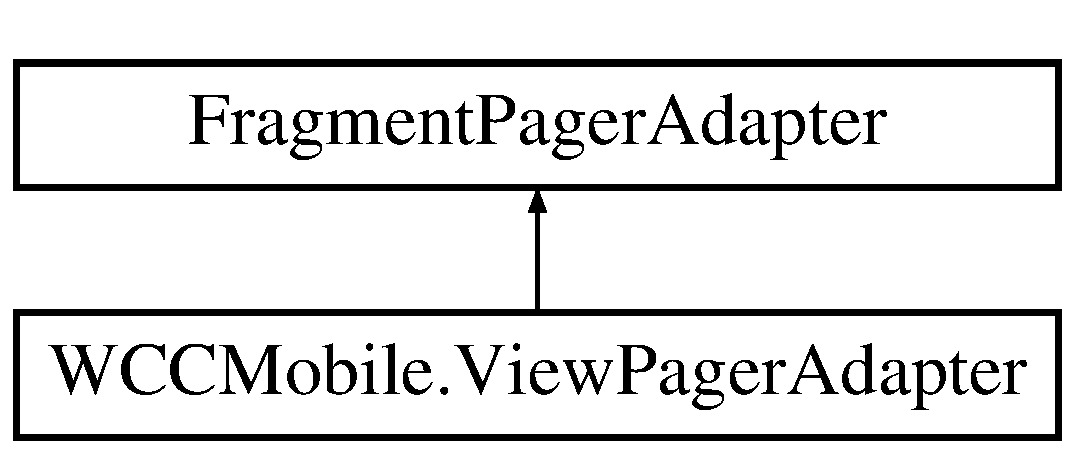
\includegraphics[height=2.000000cm]{class_w_c_c_mobile_1_1_view_pager_adapter}
\end{center}
\end{figure}
\subsection*{Public Member Functions}
\begin{DoxyCompactItemize}
\item 
\hyperlink{class_w_c_c_mobile_1_1_view_pager_adapter_ad09dbb7d5a54809a7fc3ae5901881d76}{View\+Pager\+Adapter} (Fragment\+Manager fm)
\begin{DoxyCompactList}\small\item\em Initializes a new instance of the \hyperlink{class_w_c_c_mobile_1_1_view_pager_adapter}{View\+Pager\+Adapter} class. \end{DoxyCompactList}\item 
override Java.\+Lang.\+I\+Char\+Sequence \hyperlink{class_w_c_c_mobile_1_1_view_pager_adapter_a0aed7d4fe5e6daa5da54670b9067ff69}{Get\+Page\+Title\+Formatted} (int position)
\begin{DoxyCompactList}\small\item\em Gets the page title formatted. \end{DoxyCompactList}\item 
override Fragment \hyperlink{class_w_c_c_mobile_1_1_view_pager_adapter_ac237d55d9eea2b67747dd5510bb0e8d6}{Get\+Item} (int position)
\begin{DoxyCompactList}\small\item\em Gets the item. \end{DoxyCompactList}\end{DoxyCompactItemize}
\subsection*{Static Public Attributes}
\begin{DoxyCompactItemize}
\item 
static Java\+String\mbox{[}$\,$\mbox{]} \hyperlink{class_w_c_c_mobile_1_1_view_pager_adapter_ac9cb2ad630a3ffe31a38166ae81df3ea}{Titles}
\begin{DoxyCompactList}\small\item\em The titles \end{DoxyCompactList}\end{DoxyCompactItemize}
\subsection*{Properties}
\begin{DoxyCompactItemize}
\item 
override int \hyperlink{class_w_c_c_mobile_1_1_view_pager_adapter_a6285d36f4653b2102da80b35b341dd47}{Count}\hspace{0.3cm}{\ttfamily  \mbox{[}get\mbox{]}}
\begin{DoxyCompactList}\small\item\em Gets the count. \end{DoxyCompactList}\end{DoxyCompactItemize}


\subsection{Constructor \& Destructor Documentation}
\index{W\+C\+C\+Mobile\+::\+View\+Pager\+Adapter@{W\+C\+C\+Mobile\+::\+View\+Pager\+Adapter}!View\+Pager\+Adapter@{View\+Pager\+Adapter}}
\index{View\+Pager\+Adapter@{View\+Pager\+Adapter}!W\+C\+C\+Mobile\+::\+View\+Pager\+Adapter@{W\+C\+C\+Mobile\+::\+View\+Pager\+Adapter}}
\subsubsection[{\texorpdfstring{View\+Pager\+Adapter(\+Fragment\+Manager fm)}{ViewPagerAdapter(FragmentManager fm)}}]{\setlength{\rightskip}{0pt plus 5cm}W\+C\+C\+Mobile.\+View\+Pager\+Adapter.\+View\+Pager\+Adapter (
\begin{DoxyParamCaption}
\item[{Fragment\+Manager}]{fm}
\end{DoxyParamCaption}
)}\hypertarget{class_w_c_c_mobile_1_1_view_pager_adapter_ad09dbb7d5a54809a7fc3ae5901881d76}{}\label{class_w_c_c_mobile_1_1_view_pager_adapter_ad09dbb7d5a54809a7fc3ae5901881d76}


Initializes a new instance of the \hyperlink{class_w_c_c_mobile_1_1_view_pager_adapter}{View\+Pager\+Adapter} class. 


\begin{DoxyParams}{Parameters}
{\em fm} & The fm.\\
\hline
\end{DoxyParams}


\subsection{Member Function Documentation}
\index{W\+C\+C\+Mobile\+::\+View\+Pager\+Adapter@{W\+C\+C\+Mobile\+::\+View\+Pager\+Adapter}!Get\+Item@{Get\+Item}}
\index{Get\+Item@{Get\+Item}!W\+C\+C\+Mobile\+::\+View\+Pager\+Adapter@{W\+C\+C\+Mobile\+::\+View\+Pager\+Adapter}}
\subsubsection[{\texorpdfstring{Get\+Item(int position)}{GetItem(int position)}}]{\setlength{\rightskip}{0pt plus 5cm}override Fragment W\+C\+C\+Mobile.\+View\+Pager\+Adapter.\+Get\+Item (
\begin{DoxyParamCaption}
\item[{int}]{position}
\end{DoxyParamCaption}
)}\hypertarget{class_w_c_c_mobile_1_1_view_pager_adapter_ac237d55d9eea2b67747dd5510bb0e8d6}{}\label{class_w_c_c_mobile_1_1_view_pager_adapter_ac237d55d9eea2b67747dd5510bb0e8d6}


Gets the item. 


\begin{DoxyParams}{Parameters}
{\em position} & The position.\\
\hline
\end{DoxyParams}
\begin{DoxyReturn}{Returns}

\end{DoxyReturn}
\index{W\+C\+C\+Mobile\+::\+View\+Pager\+Adapter@{W\+C\+C\+Mobile\+::\+View\+Pager\+Adapter}!Get\+Page\+Title\+Formatted@{Get\+Page\+Title\+Formatted}}
\index{Get\+Page\+Title\+Formatted@{Get\+Page\+Title\+Formatted}!W\+C\+C\+Mobile\+::\+View\+Pager\+Adapter@{W\+C\+C\+Mobile\+::\+View\+Pager\+Adapter}}
\subsubsection[{\texorpdfstring{Get\+Page\+Title\+Formatted(int position)}{GetPageTitleFormatted(int position)}}]{\setlength{\rightskip}{0pt plus 5cm}override Java.\+Lang.\+I\+Char\+Sequence W\+C\+C\+Mobile.\+View\+Pager\+Adapter.\+Get\+Page\+Title\+Formatted (
\begin{DoxyParamCaption}
\item[{int}]{position}
\end{DoxyParamCaption}
)}\hypertarget{class_w_c_c_mobile_1_1_view_pager_adapter_a0aed7d4fe5e6daa5da54670b9067ff69}{}\label{class_w_c_c_mobile_1_1_view_pager_adapter_a0aed7d4fe5e6daa5da54670b9067ff69}


Gets the page title formatted. 


\begin{DoxyParams}{Parameters}
{\em position} & The position.\\
\hline
\end{DoxyParams}
\begin{DoxyReturn}{Returns}

\end{DoxyReturn}


\subsection{Member Data Documentation}
\index{W\+C\+C\+Mobile\+::\+View\+Pager\+Adapter@{W\+C\+C\+Mobile\+::\+View\+Pager\+Adapter}!Titles@{Titles}}
\index{Titles@{Titles}!W\+C\+C\+Mobile\+::\+View\+Pager\+Adapter@{W\+C\+C\+Mobile\+::\+View\+Pager\+Adapter}}
\subsubsection[{\texorpdfstring{Titles}{Titles}}]{\setlength{\rightskip}{0pt plus 5cm}Java\+String \mbox{[}$\,$\mbox{]} W\+C\+C\+Mobile.\+View\+Pager\+Adapter.\+Titles\hspace{0.3cm}{\ttfamily [static]}}\hypertarget{class_w_c_c_mobile_1_1_view_pager_adapter_ac9cb2ad630a3ffe31a38166ae81df3ea}{}\label{class_w_c_c_mobile_1_1_view_pager_adapter_ac9cb2ad630a3ffe31a38166ae81df3ea}
{\bfseries Initial value\+:}
\begin{DoxyCode}
= \textcolor{keyword}{new}[]
        \{
            \textcolor{keyword}{new} \hyperlink{namespace_java_string}{JavaString}(\textcolor{stringliteral}{"Campus Map"}),
            \textcolor{keyword}{new} \hyperlink{namespace_java_string}{JavaString}(\textcolor{stringliteral}{"WCC Mobile Home"}),
        \}
\end{DoxyCode}


The titles 



\subsection{Property Documentation}
\index{W\+C\+C\+Mobile\+::\+View\+Pager\+Adapter@{W\+C\+C\+Mobile\+::\+View\+Pager\+Adapter}!Count@{Count}}
\index{Count@{Count}!W\+C\+C\+Mobile\+::\+View\+Pager\+Adapter@{W\+C\+C\+Mobile\+::\+View\+Pager\+Adapter}}
\subsubsection[{\texorpdfstring{Count}{Count}}]{\setlength{\rightskip}{0pt plus 5cm}override int W\+C\+C\+Mobile.\+View\+Pager\+Adapter.\+Count\hspace{0.3cm}{\ttfamily [get]}}\hypertarget{class_w_c_c_mobile_1_1_view_pager_adapter_a6285d36f4653b2102da80b35b341dd47}{}\label{class_w_c_c_mobile_1_1_view_pager_adapter_a6285d36f4653b2102da80b35b341dd47}


Gets the count. 

The count. 

The documentation for this class was generated from the following file\+:\begin{DoxyCompactItemize}
\item 
Source/\+Adapters/View\+Pager\+Adapter.\+cs\end{DoxyCompactItemize}

\hypertarget{class_w_c_c_mobile_1_1_w_c_c_mobile_action_bar_toggle}{}\section{W\+C\+C\+Mobile.\+W\+C\+C\+Mobile\+Action\+Bar\+Toggle Class Reference}
\label{class_w_c_c_mobile_1_1_w_c_c_mobile_action_bar_toggle}\index{W\+C\+C\+Mobile.\+W\+C\+C\+Mobile\+Action\+Bar\+Toggle@{W\+C\+C\+Mobile.\+W\+C\+C\+Mobile\+Action\+Bar\+Toggle}}
Inheritance diagram for W\+C\+C\+Mobile.\+W\+C\+C\+Mobile\+Action\+Bar\+Toggle\+:\begin{figure}[H]
\begin{center}
\leavevmode
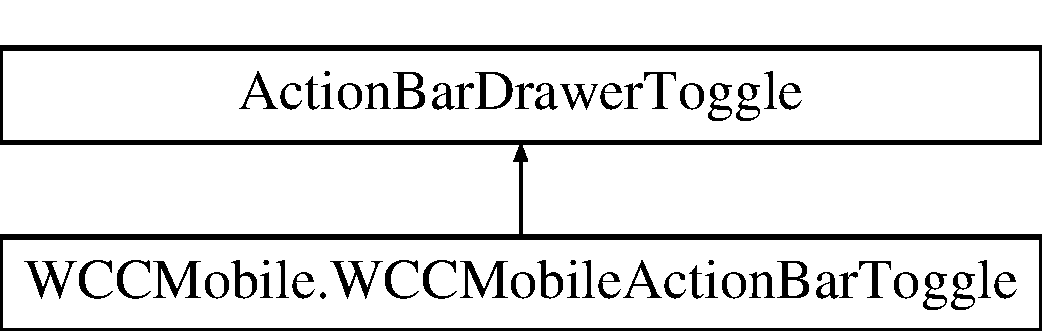
\includegraphics[height=2.000000cm]{class_w_c_c_mobile_1_1_w_c_c_mobile_action_bar_toggle}
\end{center}
\end{figure}
\subsection*{Public Member Functions}
\begin{DoxyCompactItemize}
\item 
\hyperlink{class_w_c_c_mobile_1_1_w_c_c_mobile_action_bar_toggle_a26328b707632ee12dba2d833f8a03dc0}{W\+C\+C\+Mobile\+Action\+Bar\+Toggle} (Activity activity, Drawer\+Layout drawer, int open\+Drawer\+Content\+Res, int close\+Drawer\+Content\+Rest)
\item 
override void \hyperlink{class_w_c_c_mobile_1_1_w_c_c_mobile_action_bar_toggle_acaababedc91f67db74e8d6811b7fa061}{On\+Drawer\+Opened} (View drawer\+View)
\begin{DoxyCompactList}\small\item\em Called when \mbox{[}drawer opened\mbox{]}. \end{DoxyCompactList}\item 
override void \hyperlink{class_w_c_c_mobile_1_1_w_c_c_mobile_action_bar_toggle_ab3e592f17cb6b208ae226e0f6263c47d}{On\+Drawer\+Closed} (View drawer\+View)
\begin{DoxyCompactList}\small\item\em Called when \mbox{[}drawer closed\mbox{]}. \end{DoxyCompactList}\end{DoxyCompactItemize}
\subsection*{Properties}
\begin{DoxyCompactItemize}
\item 
Action \hyperlink{class_w_c_c_mobile_1_1_w_c_c_mobile_action_bar_toggle_ab67f063b3a4e7896fc8cd982b24952e0}{Open\+Callback}\hspace{0.3cm}{\ttfamily  \mbox{[}get, set\mbox{]}}
\begin{DoxyCompactList}\small\item\em Gets or sets the open callback. \end{DoxyCompactList}\item 
Action \hyperlink{class_w_c_c_mobile_1_1_w_c_c_mobile_action_bar_toggle_aea8db24fab6dffb838f246cf4704b804}{Close\+Callback}\hspace{0.3cm}{\ttfamily  \mbox{[}get, set\mbox{]}}
\begin{DoxyCompactList}\small\item\em Gets or sets the close callback. \end{DoxyCompactList}\end{DoxyCompactItemize}


\subsection{Constructor \& Destructor Documentation}
\index{W\+C\+C\+Mobile\+::\+W\+C\+C\+Mobile\+Action\+Bar\+Toggle@{W\+C\+C\+Mobile\+::\+W\+C\+C\+Mobile\+Action\+Bar\+Toggle}!W\+C\+C\+Mobile\+Action\+Bar\+Toggle@{W\+C\+C\+Mobile\+Action\+Bar\+Toggle}}
\index{W\+C\+C\+Mobile\+Action\+Bar\+Toggle@{W\+C\+C\+Mobile\+Action\+Bar\+Toggle}!W\+C\+C\+Mobile\+::\+W\+C\+C\+Mobile\+Action\+Bar\+Toggle@{W\+C\+C\+Mobile\+::\+W\+C\+C\+Mobile\+Action\+Bar\+Toggle}}
\subsubsection[{\texorpdfstring{W\+C\+C\+Mobile\+Action\+Bar\+Toggle(\+Activity activity, Drawer\+Layout drawer, int open\+Drawer\+Content\+Res, int close\+Drawer\+Content\+Rest)}{WCCMobileActionBarToggle(Activity activity, DrawerLayout drawer, int openDrawerContentRes, int closeDrawerContentRest)}}]{\setlength{\rightskip}{0pt plus 5cm}W\+C\+C\+Mobile.\+W\+C\+C\+Mobile\+Action\+Bar\+Toggle.\+W\+C\+C\+Mobile\+Action\+Bar\+Toggle (
\begin{DoxyParamCaption}
\item[{Activity}]{activity, }
\item[{Drawer\+Layout}]{drawer, }
\item[{int}]{open\+Drawer\+Content\+Res, }
\item[{int}]{close\+Drawer\+Content\+Rest}
\end{DoxyParamCaption}
)}\hypertarget{class_w_c_c_mobile_1_1_w_c_c_mobile_action_bar_toggle_a26328b707632ee12dba2d833f8a03dc0}{}\label{class_w_c_c_mobile_1_1_w_c_c_mobile_action_bar_toggle_a26328b707632ee12dba2d833f8a03dc0}





\begin{DoxyParams}{Parameters}
{\em activity} & \\
\hline
{\em drawer} & \\
\hline
{\em open\+Drawer\+Content\+Res} & \\
\hline
{\em close\+Drawer\+Content\+Rest} & \\
\hline
\end{DoxyParams}


\subsection{Member Function Documentation}
\index{W\+C\+C\+Mobile\+::\+W\+C\+C\+Mobile\+Action\+Bar\+Toggle@{W\+C\+C\+Mobile\+::\+W\+C\+C\+Mobile\+Action\+Bar\+Toggle}!On\+Drawer\+Closed@{On\+Drawer\+Closed}}
\index{On\+Drawer\+Closed@{On\+Drawer\+Closed}!W\+C\+C\+Mobile\+::\+W\+C\+C\+Mobile\+Action\+Bar\+Toggle@{W\+C\+C\+Mobile\+::\+W\+C\+C\+Mobile\+Action\+Bar\+Toggle}}
\subsubsection[{\texorpdfstring{On\+Drawer\+Closed(\+View drawer\+View)}{OnDrawerClosed(View drawerView)}}]{\setlength{\rightskip}{0pt plus 5cm}override void W\+C\+C\+Mobile.\+W\+C\+C\+Mobile\+Action\+Bar\+Toggle.\+On\+Drawer\+Closed (
\begin{DoxyParamCaption}
\item[{View}]{drawer\+View}
\end{DoxyParamCaption}
)}\hypertarget{class_w_c_c_mobile_1_1_w_c_c_mobile_action_bar_toggle_ab3e592f17cb6b208ae226e0f6263c47d}{}\label{class_w_c_c_mobile_1_1_w_c_c_mobile_action_bar_toggle_ab3e592f17cb6b208ae226e0f6263c47d}


Called when \mbox{[}drawer closed\mbox{]}. 


\begin{DoxyParams}{Parameters}
{\em drawer\+View} & The drawer view.\\
\hline
\end{DoxyParams}
\index{W\+C\+C\+Mobile\+::\+W\+C\+C\+Mobile\+Action\+Bar\+Toggle@{W\+C\+C\+Mobile\+::\+W\+C\+C\+Mobile\+Action\+Bar\+Toggle}!On\+Drawer\+Opened@{On\+Drawer\+Opened}}
\index{On\+Drawer\+Opened@{On\+Drawer\+Opened}!W\+C\+C\+Mobile\+::\+W\+C\+C\+Mobile\+Action\+Bar\+Toggle@{W\+C\+C\+Mobile\+::\+W\+C\+C\+Mobile\+Action\+Bar\+Toggle}}
\subsubsection[{\texorpdfstring{On\+Drawer\+Opened(\+View drawer\+View)}{OnDrawerOpened(View drawerView)}}]{\setlength{\rightskip}{0pt plus 5cm}override void W\+C\+C\+Mobile.\+W\+C\+C\+Mobile\+Action\+Bar\+Toggle.\+On\+Drawer\+Opened (
\begin{DoxyParamCaption}
\item[{View}]{drawer\+View}
\end{DoxyParamCaption}
)}\hypertarget{class_w_c_c_mobile_1_1_w_c_c_mobile_action_bar_toggle_acaababedc91f67db74e8d6811b7fa061}{}\label{class_w_c_c_mobile_1_1_w_c_c_mobile_action_bar_toggle_acaababedc91f67db74e8d6811b7fa061}


Called when \mbox{[}drawer opened\mbox{]}. 


\begin{DoxyParams}{Parameters}
{\em drawer\+View} & The drawer view.\\
\hline
\end{DoxyParams}


\subsection{Property Documentation}
\index{W\+C\+C\+Mobile\+::\+W\+C\+C\+Mobile\+Action\+Bar\+Toggle@{W\+C\+C\+Mobile\+::\+W\+C\+C\+Mobile\+Action\+Bar\+Toggle}!Close\+Callback@{Close\+Callback}}
\index{Close\+Callback@{Close\+Callback}!W\+C\+C\+Mobile\+::\+W\+C\+C\+Mobile\+Action\+Bar\+Toggle@{W\+C\+C\+Mobile\+::\+W\+C\+C\+Mobile\+Action\+Bar\+Toggle}}
\subsubsection[{\texorpdfstring{Close\+Callback}{CloseCallback}}]{\setlength{\rightskip}{0pt plus 5cm}Action W\+C\+C\+Mobile.\+W\+C\+C\+Mobile\+Action\+Bar\+Toggle.\+Close\+Callback\hspace{0.3cm}{\ttfamily [get]}, {\ttfamily [set]}}\hypertarget{class_w_c_c_mobile_1_1_w_c_c_mobile_action_bar_toggle_aea8db24fab6dffb838f246cf4704b804}{}\label{class_w_c_c_mobile_1_1_w_c_c_mobile_action_bar_toggle_aea8db24fab6dffb838f246cf4704b804}


Gets or sets the close callback. 

The close callback. \index{W\+C\+C\+Mobile\+::\+W\+C\+C\+Mobile\+Action\+Bar\+Toggle@{W\+C\+C\+Mobile\+::\+W\+C\+C\+Mobile\+Action\+Bar\+Toggle}!Open\+Callback@{Open\+Callback}}
\index{Open\+Callback@{Open\+Callback}!W\+C\+C\+Mobile\+::\+W\+C\+C\+Mobile\+Action\+Bar\+Toggle@{W\+C\+C\+Mobile\+::\+W\+C\+C\+Mobile\+Action\+Bar\+Toggle}}
\subsubsection[{\texorpdfstring{Open\+Callback}{OpenCallback}}]{\setlength{\rightskip}{0pt plus 5cm}Action W\+C\+C\+Mobile.\+W\+C\+C\+Mobile\+Action\+Bar\+Toggle.\+Open\+Callback\hspace{0.3cm}{\ttfamily [get]}, {\ttfamily [set]}}\hypertarget{class_w_c_c_mobile_1_1_w_c_c_mobile_action_bar_toggle_ab67f063b3a4e7896fc8cd982b24952e0}{}\label{class_w_c_c_mobile_1_1_w_c_c_mobile_action_bar_toggle_ab67f063b3a4e7896fc8cd982b24952e0}


Gets or sets the open callback. 

The open callback. 

The documentation for this class was generated from the following file\+:\begin{DoxyCompactItemize}
\item 
Source/\+Activities/Campus\+Map\+Activity.\+cs\end{DoxyCompactItemize}

\hypertarget{class_w_c_c_mobile_1_1_resources_1_1_yellow_book_adapter}{}\section{W\+C\+C\+Mobile.\+Resources.\+Yellow\+Book\+Adapter Class Reference}
\label{class_w_c_c_mobile_1_1_resources_1_1_yellow_book_adapter}\index{W\+C\+C\+Mobile.\+Resources.\+Yellow\+Book\+Adapter@{W\+C\+C\+Mobile.\+Resources.\+Yellow\+Book\+Adapter}}
Inheritance diagram for W\+C\+C\+Mobile.\+Resources.\+Yellow\+Book\+Adapter\+:\begin{figure}[H]
\begin{center}
\leavevmode
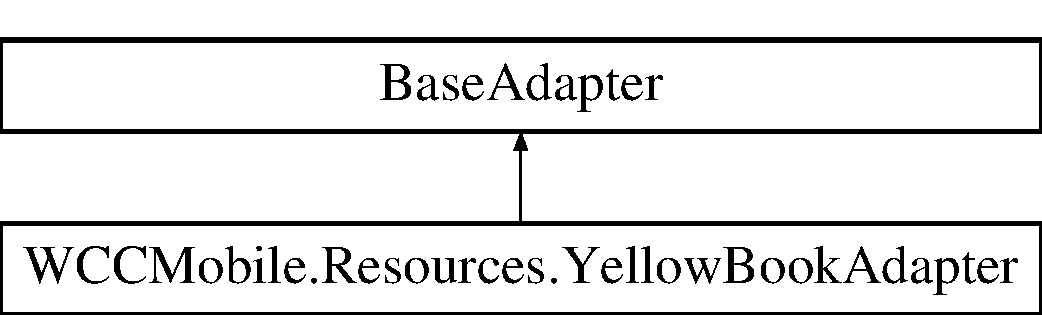
\includegraphics[height=2.000000cm]{class_w_c_c_mobile_1_1_resources_1_1_yellow_book_adapter}
\end{center}
\end{figure}
\subsection*{Public Member Functions}
\begin{DoxyCompactItemize}
\item 
{\bfseries Yellow\+Book\+Adapter} (Context c)\hypertarget{class_w_c_c_mobile_1_1_resources_1_1_yellow_book_adapter_a5b67f8b8472369aba09dfb7784289256}{}\label{class_w_c_c_mobile_1_1_resources_1_1_yellow_book_adapter_a5b67f8b8472369aba09dfb7784289256}

\item 
override Java.\+Lang.\+Object {\bfseries Get\+Item} (int position)\hypertarget{class_w_c_c_mobile_1_1_resources_1_1_yellow_book_adapter_ad49d89254441016787d74c4300722d44}{}\label{class_w_c_c_mobile_1_1_resources_1_1_yellow_book_adapter_ad49d89254441016787d74c4300722d44}

\item 
override long {\bfseries Get\+Item\+Id} (int position)\hypertarget{class_w_c_c_mobile_1_1_resources_1_1_yellow_book_adapter_a9dfaeb0e011baf1c34a53dd32b0dc49a}{}\label{class_w_c_c_mobile_1_1_resources_1_1_yellow_book_adapter_a9dfaeb0e011baf1c34a53dd32b0dc49a}

\item 
override View {\bfseries Get\+View} (int position, View convert\+View, View\+Group parent)\hypertarget{class_w_c_c_mobile_1_1_resources_1_1_yellow_book_adapter_ad2054ed1b424cb960605d4b4f83df5d5}{}\label{class_w_c_c_mobile_1_1_resources_1_1_yellow_book_adapter_ad2054ed1b424cb960605d4b4f83df5d5}

\end{DoxyCompactItemize}
\subsection*{Properties}
\begin{DoxyCompactItemize}
\item 
override int {\bfseries Count}\hspace{0.3cm}{\ttfamily  \mbox{[}get\mbox{]}}\hypertarget{class_w_c_c_mobile_1_1_resources_1_1_yellow_book_adapter_a4e7b56a6095169557525a89edfa4036c}{}\label{class_w_c_c_mobile_1_1_resources_1_1_yellow_book_adapter_a4e7b56a6095169557525a89edfa4036c}

\item 
static Dictionary$<$ int, string $>$ {\bfseries get\+Book}\hspace{0.3cm}{\ttfamily  \mbox{[}get\mbox{]}}\hypertarget{class_w_c_c_mobile_1_1_resources_1_1_yellow_book_adapter_a80f62c0acae6f6587de2f7f311f8961f}{}\label{class_w_c_c_mobile_1_1_resources_1_1_yellow_book_adapter_a80f62c0acae6f6587de2f7f311f8961f}

\end{DoxyCompactItemize}


The documentation for this class was generated from the following file\+:\begin{DoxyCompactItemize}
\item 
Source/\+Adapters/Yellow\+Book\+Adapter.\+cs\end{DoxyCompactItemize}

%--- End generated contents ---

% Index
\backmatter
\newpage
\phantomsection
\clearemptydoublepage
\addcontentsline{toc}{chapter}{Index}
\printindex

\end{document}
